\documentclass[10pt]{mypackage}

\usepackage[uprightgreeks,light,noDcommand]{kpfonts}
\renewcommand{\coloneq}{\coloneqq}
\renewcommand{\eqcolon}{\eqqcolon}
%\renewcommand{\mathbb}{\mathds}
\usepackage{homework}
\usepackage{notes}

%\usepackage[ backend=bibtex, style = alphabetic, sorting=ynt ]{biblatex}
%\addbibresource{  }

\usepackage{parskip}

\fancyhf{}
\fancyhead[R]{Avinash Iyer}
\fancyhead[L]{}
\fancyfoot[C]{\thepage}

\setcounter{secnumdepth}{0}

\begin{document}
\RaggedRight
\section{Group Theory}%
\subsection{Group Theory Notes}%
\subsubsection{Useful Facts}%
\begin{itemize}
  \item Let $G$ be a finite group, and suppose $G$ acts on itself by conjugation. Then, the stabilizer of $x\in G$ is denoted $C_G(x)$, and by the orbit-stabilizer theorem, it follows that the number of \textit{elements} of the conjugacy class of $x$, $K_G(x)$, is given by $\left[ G:C_G(x) \right]$. The \textit{class equation} says we may find
    \begin{align*}
      \left\vert G \right\vert &= \left\vert Z(G) \right\vert + \sum_{i=1}^{r} \left[ G:C_G\left( x_i \right) \right],
    \end{align*}
    where $\set{x_1,\dots,x_r}$ is a family of representatives of conjugacy classes.
  \item If $G$ acts on its \textit{subgroups} by conjugation, then the \textit{normalizer} of $H\leq G$, denoted $N_G(H)$, is the stabilizer of $H$ under conjugation. Similarly, number of subgroups conjugate to $H\leq G$ is given by $\left[ G:N_G(H) \right]$.
  \item If $H\trianglelefteq G$ is a normal subgroup, then $G$ acts on $H$ by conjugation. The corresponding permutation $\rho\colon G\rightarrow \aut\left( H \right)$ has kernel $C_G(H)$, where
    \begin{align*}
      C_G(H) &= \set{g\in G : ghg^{-1} = h\text{ for all }h\in H}.
    \end{align*}
  \item A subgroup $H\leq G$ is called \textit{characteristic} if $\sigma(H) = H$ for all automorphisms $\sigma\in \aut\left( G \right)$. If $K\leq H\trianglelefteq G$ is a chain of subgroups with $K$ characteristic in $H$, while $H$ is normal in $G$, then $K\trianglelefteq G$ is normal.

    The subgroups $\left[ G,G \right]$ and $Z(G)$ are characteristic in $G$.
  \item Every $p$-group has nontrivial center.
  \item If $G$ acts on a set $X$, and $H$ is the stabilizer subgroup of some $x\in X$, then if $\rho\colon G\rightarrow \sym\left( X \right)$ is the permutation representation for this action, then $\ker\left( \rho \right) \leq H$.
  \item If $P_1,\dots,P_r$ are $p$-Sylow subgroups of $G$, they are all conjugate to each other, and the normalizer $N_G\left( P_i \right)$ is a conjugate of $N_G\left( P_j \right)$ for $1\leq i,j \leq r$.
  \item Every conjugacy class in the symmetric group $S_n$ is given by the cycle type. Moreover, given an element $\sigma\in A_n$, the conjugacy classes $K_{A_n}\left(\sigma\right) = K_{S_n}\left(\sigma\right)$ if and only if there is an odd permutation in the centralizer $C_{S_n}\left(\sigma\right)$. If there is no odd permutation in $C_{S_n}\left(\sigma\right)$, then the conjugacy class $K_{S_n}\left(\sigma\right)$ splits into two separate conjugacy classes over $A_n$.
\end{itemize}

\subsubsection{Semidirect Products}%
Suppose $N$ and $H$ are subgroups of a group $G$, where $N$ is normal and $H$ is such that $N\cap H = \set{e}$. We will obtain a description of the structure of $G$ in terms of the structure of $N$ and $H$.

A short exact sequence of groups is a sequence of groups and homomorphisms
\begin{align*}
  1 \rightarrow N \xrightarrow{\varphi} G \xrightarrow{\psi} H \rightarrow 1
\end{align*}
where $\psi$ is surjective and $\varphi$ identifies $N$ with $\ker\left( \psi \right)$. In other words, the sequence is exact if $N$ is normal in $G$ and $\psi$ induces an isomorphism $G/N\cong H$.
\begin{definition}
  Let $N$ and $H$ be groups. A group $G$ is an \textit{extension} of $H$ by $N$ if there is an exact sequence of groups
  \begin{align*}
    1 \rightarrow N\rightarrow G\rightarrow H\rightarrow 1.
  \end{align*}
  The exact sequence is said to split if $H$ can be identified with a subgroup of $G$, so that $N\cap H = \set{e}$.
\end{definition}
If $N$ is normal, then observe that any subgroup $H$ of $G$ acts on $N$ by conjugation; furthermore, conjugation determines a homomorphism
\begin{align*}
  \iota\colon H\rightarrow \aut\left( N \right)
\end{align*}
given by $h\mapsto \iota_h$, where $\iota_h(n) = hnh^{-1}$.

Now, we consider a certain tautology. If $G = NH$ with $N\cap H = \set{e}$ and $N$ normal, then observe that
\begin{align*}
  n_1h_1n_2h_2 &= \left( n_1\left( h_1n_2h_1^{-1} \right) \right)\left( h_1h_2 \right).
\end{align*}
In particular, if we know the conjugation action of $H$ on $N$, then we can recover the operation in $G$ from this information and the operations in $N$ and $H$.

This allows us to construct semidirect products by considering any two arbitrary groups $N$ and $H$ with an arbitrary group homomorphism
\begin{align*}
  \theta\colon H&\rightarrow \aut\left( N \right)\\
  h &\mapsto \theta_h.
\end{align*}
Then, we may define an operation on $N\times H$ by taking
\begin{align*}
  \left( n_1,h_1 \right)\cdot \left( n_2,h_2 \right) &= \left( n_1\theta_{h_1}\left(n_2\right), h_1h_2 \right).
\end{align*}
Observe that in the special case where $N,H\leq G$ with $G = NH$, $N$ normal, and $N\cap H = \set{e}$, the operation $\theta$ can be given by the map $\iota$. The group $\left( N\times H,\cdot \right)$ is denoted $N\rtimes_{\theta}H$, and is called the semidirect product of $N$ and $H$ with respect to $\theta$. Observe that the ordinary direct product is a semidirect product where $\theta$ is the trivial map.

We will discuss some examples.
\begin{enumerate}[(i)]
  \item If $G$ has a normal subgroup $K$ of order $n$ and a subgroup $H$ of order $m$, with $HK = G$, $H\cap K = \set{e}$, and $\gcd\left( m,\left\vert \Aut\left( K \right) \right\vert \right) = 1$, then $G\cong H\times K$.
  \item Suppose $H$ is an abelian group of arbitrary order, and let $K = \Z/2\Z$. Define $\varphi\colon K\rightarrow \aut(H)$ by inversion. Then, $G = H\rtimes K$ contains the subgroup $H$ of index $2$, with $xhx^{-1} = h^{-1}$ for all $h\in H$ and $e\neq x\in K$.
    
    When $H\cong \Z/n\Z$, this yields the dihedral group $D_n$ of order $2n$, while if $H \cong \Z$, we have the infinite dihedral group $D_{\infty}$.
  \item If $H$ is a group, and $K = \aut\left( H \right)$, then $\varphi\colon K\rightarrow \aut\left( H \right)$ given by the identity yields the semidirect product $H\rtimes \aut\left( H \right)$, denoted the \textit{holomorph} of $H$.
\end{enumerate}

\subsubsection{Solvable Groups}%
\begin{definition}
  A series of subgroups $G_i$ of a group $G$ is a decreasing sequence of subgroups
  \begin{align*}
    G = G_0\triangleright G_1\triangleright G_2\supsetneq\cdots,
  \end{align*}
  where the length of the series is the number of strict inclusions.

  A normal series is a series of subgroups where $G_{i+1}\trianglelefteq G_i$ for each $i$. The number $\ell(G)$ is the length of a maximal normal series.

  A \textit{composition series} is a normal series
  \begin{align*}
    G = G_0\triangleright G_1\triangleright\cdots\triangleright G_n = \set{e}
  \end{align*}
  where the successive quotients $G_i/G_{i+1}$ are simple.
\end{definition}
\begin{theorem}[Jordan--Hölder Theorem]
  Let $G$ be a group, and suppose there are two composition series
  \begin{align*}
    G = G_0\supsetneq G_1\supsetneq G_2\supsetneq\cdots\supsetneq G_n = \set{e}\\
    G = G_0'\supsetneq G_1'\supsetneq G_2'\supsetneq\cdots\supsetneq G_m = \set{e}.
  \end{align*}
  Then, $m = n$, and the quotient groups $H_i = G_i/G_{i+1}$ and $H_i' = G_i'/G_{i+1}'$ agree up to isomorphism and permutation.
\end{theorem}
\begin{proof}
  Considering the following composition series
  \begin{align*}
    G = G_0\supsetneq G_1\supsetneq G_2\supsetneq\cdots\supsetneq G_n = \set{e}
  \end{align*}
  we induct on $n$. If $n = 0$, then $G$ is trivial and there is nothing to prove.

  Suppose $n > 0$, and consider another composition series
  \begin{align*}
    G = G_0'\supsetneq G_1'\supsetneq G_2'\supsetneq\cdots\supsetneq G_m' = \set{e}.
  \end{align*}
  If $G_1 = G_1'$, then the result follows from the induction hypothesis since $G_1$ has a composition series of length $n-1$.

  Therefore, we may assume that $G_1 \neq G_1'$. We observe that $G_1G_1' = G$, since $G_1G_1'$ is normal in $G$ and $G_1\supsetneq G_1G_1'$, but there are no proper normal subgroups between $G_1$ and $G$ since $G/G_1$ is simple.

  Consider the group $K = G_1\cap G_1'$. The distinct subgroups $G_i\cap K$ determine a composition series
  \begin{align*}
    K \supsetneq K_1\supsetneq K_2\supsetneq \cdots\supsetneq K_r = \set{e}.
  \end{align*}
  By the Second Isomorphism Theorem, we have
  \begin{align*}
    \frac{G_1}{K} &= \frac{G_1}{G_1\cap G_1'}\\
                  &\cong \frac{G_1G_1'}{G_1'}\\
                  &= \frac{G}{G_1'}
  \end{align*}
  and $G_1'/K \cong G/G_1$. These quotients are simple, so we obtain two new composition series
  \begin{align*}
    G \supsetneq G_1 \supsetneq K \supsetneq K_1\supsetneq\cdots\supsetneq \set{e}\\
    G\supsetneq G_1'\supsetneq K \supsetneq K_1 \supsetneq \cdots\supsetneq \set{e}.
  \end{align*}
  These composition series only differ at the first step. The two series have the same length and the same quotients. Next, we claim that the first of these series has the same length and quotients of the original series. Since
  \begin{align*}
    G_1\supsetneq K\supsetneq K_1\supsetneq K_2\supsetneq\cdots\supsetneq K_r = \set{e}
  \end{align*}
  is a composition series for $G_1$, the induction hypothesis gives that it must have the same length and quotients as the composition series
  \begin{align*}
    G_1\supsetneq G_2\supsetneq \cdots \supsetneq G_n = \set{e}.
  \end{align*}
  Therefore, applying the induction hypothesis, it follows that the series
  \begin{align*}
    G_1'\supsetneq K \supsetneq K_1\supsetneq K_2\supsetneq \cdots \supsetneq K_r = \set{e}
  \end{align*}
  has the same length and quotients as 
  \begin{align*}
    G_1'\supsetneq G_2'\supsetneq\cdots\supsetneq G_m' = \set{e}.
  \end{align*}
\end{proof}
\begin{proposition}
  Let $G$ be a group, and let $N$ be a normal subgroup of $G$. Then, $G$ has a composition series if and only if $N$ and $G/N$ have composition series. Furthermore,
  \begin{align*}
    \ell\left( G \right) &= \ell\left( N \right) + \ell\left( G/N \right),
  \end{align*}
  and the composition factors of $G$ consist of the composition factors of $N$ and of $G/N$.
\end{proposition}
\begin{proof}
  If $G/N$ has a composition series, then the subgroups appearing in it correspond to subgroups of $G$ containing $N$ with isomorphic quotients. Therefore, if both $G/N$ and $N$ have composition series, concatenating produces a composition series for $G$.

  For the converse, suppose $G$ has a composition series
  \begin{align*}
    G &= G_0\supsetneq G_1\supsetneq G_2\supsetneq \cdots \supsetneq G_n = \set{e},
  \end{align*}
  and that $N$ is a normal subgroup of $G$. Taking intersections with $N$ gives a sequence of subgroups
  \begin{align*}
    N = G\cap N \supseteq G_1\cap N \supsetneq \cdots \supsetneq \set{e}\cap N = \set{e}
  \end{align*}
  such that $G_{i+1}\cap N$ is normal in $G_i\cap N$ for all $i$. We claim that this is a composition series upon deleting repetitions. For this, we will establish that the quotients $\left( G_{i}\cap N \right)/\left( G_{i+1}\cap N \right)$ are either trivial or isomorphic to $G_i/G_{i+1}$. Consider the homomorphism
  \begin{align*}
    G_i\cap N \hookrightarrow G_i\rightarrow \frac{G_i}{G_{i+1}}.
  \end{align*}
  The kernel is $G_{i+1}\cap N$, so by the first isomorphism theorem, we have an injective homomorphism
  \begin{align*}
    \frac{G_{i}\cap N}{G_{i+1}\cap N} \hookrightarrow \frac{G_i}{G_{i+1}},
  \end{align*}
  where we identify the image with a subgroup of $G_i/G_{i+1}$. This subgroup is normal since $N$ is normal in $G$, and since $G_i/G_{i+1}$ is simple, we get our desired result.

  As for $G/N$, we have the composition series
  \begin{align*}
    \frac{G}{N} \supseteq \frac{G_1N}{N} \supseteq \frac{G_2N}{N}\supseteq\cdots \supseteq \set{e_{G/N}}.
  \end{align*}
  such that $\left( G_{i+1}N \right)/N$ is normal in $\left( G_iN \right)/N$. By the third isomorphism theorem, the quotients
  \begin{align*}
    \frac{\left( G_{i}N \right)/N}{\left( G_{i+1}N \right)/N} &\cong \frac{G_iN}{G_{i+1}N}
  \end{align*}
  are isomorphic. Considering the homomorphism 
  \begin{align*}
    G_i\hookrightarrow G_{i}N \rightarrow\frac{G_iN}{G_{i+1}N},
  \end{align*}
  we have that this homomorphism is surjective, and the subgroup $G_{i+1}$ of the source is sent to the identity of the target. By the first isomorphism theorem, there is a surjective homomorphism
  \begin{align*}
    \frac{G_{i}}{G_{i+1}} \rightarrow \frac{G_iN}{G_{i+1}N},
  \end{align*}
  so that $G_iN/G_{i+1}N$ is either trivial or isomorphic to it as $G_i/G_{i+1}$ is simple.
\end{proof}
Composition series are the first major step in understanding the structure of groups. Next, we consider a special series known as the \textit{derived series}.
\begin{definition}
  If $G$ is a group, then the commutator subgroup, denoted $G'$ or $\left[ G,G \right]$, is the subgroup generated by all the commutators $\left[ g,h \right] = ghg^{-1}h^{-1}$.
\end{definition}
The following follows directly from the definitions of the commutator subgroup.
\begin{theorem}
  If $G$ is a group, and $G'$ is its commutator subgroup, then
  \begin{enumerate}[(i)]
    \item $G'$ is normal in $G$ (in fact, $G'$ is \textit{characteristic} in $G$);
    \item the quotient $G/G'$ is commutative;
    \item $G'$ yields the ``maximal abelian quotient,'' in the sense that if $N\trianglelefteq G$ is another normal subgroup with $G/N$ commutative, then $G'\leq G$.
  \end{enumerate}
\end{theorem}
\begin{definition}
  The \textit{derived series} is a descending sequence of subgroups
  \begin{align*}
    G\supseteq G' \supseteq G'' \supseteq G''' \supseteq \cdots.
  \end{align*}
\end{definition}
Note that if $G$ is commutative, then the sequence automatically hits $\set{e}$, and if $G$ is simple and noncommutative, then $G = G' = G'' = \cdots$.
\begin{definition}
  A group is called \textit{solvable} if its derived series terminates in the identity.
\end{definition}
We call a normal series abelian (resp.\,cyclic) if all the quotients are abelian (resp.\,cyclic).
\begin{proposition}
  For a finite group $G$, the following are equivalent:
  \begin{enumerate}[(i)]
    \item all composition factors of $G$ are cyclic;
    \item $G$ admits a cyclic series ending in $\set{e}$;
    \item $G$ admits an abelian series ending in $\set{e}$;
    \item $G$ is solvable.
  \end{enumerate}
\end{proposition}
\begin{proof}
  Observe that (i) implies (ii) and (ii) implies (iii) follow immediately from the definition. Furthermore, (iii) implies (i) by refining an abelian series to a composition series into a family of cyclic $p$-groups. Furthermore, (iv) implies (iii) immediately from the fact that the derived series is an abelian series.

  Therefore, we must show that (iii) implies (iv). Consider an abelian series
  \begin{align*}
    G = G_0\supsetneq G_1\supsetneq G_1\supsetneq \cdots \supsetneq G_n = \set{e}.
  \end{align*}
  Then, we claim that $G^{(i)}\subseteq G_i$, where $G^{(i)}$ denotes the $i$th iterated commutator subgroup.

  This follows by induction. Since $G/G_1$ is commutative, it follows that $G'\subseteq G_1$. Since $G_i/G_{i+1}$ is abelian, it follows that $G_i'\subseteq G_{i+1}$, so that
  \begin{align*}
    G^{(i+1)} &= \left( G^{(i)} \right)'\\
              &\subseteq G_i'\\
              &\subseteq G_{i+1}.
  \end{align*}
  Therefore, we have that $G^{(n)}\subseteq G_n = \set{e}$, so that the derived series terminates at $\set{e}$.
\end{proof}
We will now discuss an application of solvability to understanding the structure of certain subgroups of the symmetric group. This has applications to Galois theory.
\begin{proposition}
  Let $p$ be prime. Then, any solvable subgroup of $S_p$ with order divisible by $p$ is contained in the normalizer of a $p$-Sylow subgroup of $S_p$. Furthermore, any such $p$-Sylow subgroup of $S_p$ is a Frobenius group of order $p\left( p-1 \right)$.
\end{proposition}
\begin{proof}
  If $G$ is a solvable subgroup of $S_p$ with order divisible by $p$, then there exists a $p$-Sylow subgroup $P = \left\langle \sigma \right\rangle$ for some $p$-cycle $\sigma$. We will start by showing the second assertion.

  If we identify the points that $P$ acts on with $\F_p$, then we may take $\sigma = \left( x\xmapsto{t_1} x + 1 \right)$. Observe that a permutation $\pi$ that commutes with $\sigma$ takes $\pi\left( x+1 \right) = \pi(x) + 1$; if $\pi(0) = c$, then $\pi = t_c$, meaning that $C_{S_p}(P) = P$, which has order $p$. There is thus an embedding $N_{S_p}(P)/P\hookrightarrow \aut\left( \Z/p\Z \right)$, which is isomorphic to $\Z/\left( p-1 \right)\Z$. Observe that the dilations $x\xmapsto{m_a}ax$ define every automorphism of $\Z/p\Z$, the automorphisms of $P$, $\sigma\mapsto \sigma^{a}$, are implemented by conjugation $m_at_1m_a^{-1} = t_a$. Thus, we have that
  \begin{align*}
    N_{S_p}(P) &= P\rtimes \left\langle \text{dilations} \right\rangle\\
               &= \Z/p\Z\rtimes \Z/\left( p-1 \right)\Z.
  \end{align*}
  Now, we will show that if $G$ is a solvable subgroup of $S_p$, then there is exactly one $p$-Sylow subgroup. First, observe that in the derived series, the group $G^{(n-1)}$ has $\left[ G^{(n-1)},G^{(n-1)} \right] = D^{(n)}(G) = 1$, so that $G^{(n-1)}$ is abelian. Since every derived subgroup is characteristic, $G^{(n-1)}$ is normal in $G$.

  Consider the stabilizer $H$ of $0\in \F_p$. The index of $H$ is $p$, and observe that the group $G^{(n-1)}H$ is a subgroup of $G$ that contains $H$, meaning that $\left[ G:G^{(n-1)}H \right]$ divides $p$, so it is equal to either $1$ or $p$. If $G^{(n-1)}H = H$, then $G^{(n-1)}\leq H$, so $G^{(n-1)}$ fixes $0$, meaning $G^{(n-1)}$ fixes all of $\F_p$, implying that $G^{(n-1)}$ is contained in the kernel of a faithful action --- specifically, the faithful action of $S_p$ on $\F_p$ --- so that $G^{(n-1)}H = G$.

  By the second isomorphism theorem, we have
  \begin{align*}
    \left[ G^{(n-1)}:G^{(n-1)}\cap H \right] &= \left[ G^{(n-1)}H:H \right]\\
                                                   &= \left[ G:H \right]\\
                                                   &= p,
  \end{align*}
  whence the size of a $G^{(n-1)}$-orbit of $0$ has size $p$, so that $G^{(n-1)}$ is transitive.

  Set $A_0 = G^{(n-1)}\cap H$. We will show that $A_0 = 1$, which occurs from showing that the intersection is normal in $G$ and the fact that a normal subgroup fixing any point fixes all points. Observe that $G^{(n-1)}$ is abelian, so $A_0$ is normal in $G^{(n-1)}$. Furthermore, if $h\in H$ and $a\in A_0$, then $hah^{-1}\in G^{(n-1)}$ since $G^{(n-1)}$ is normal in $G$, and $hah^{-1}$ fixes $0$ since all three of $h^{-1}$, $a$, and $h$ fix $0$. Therefore, $A_0$ is normal in $H$. In particular, this means that $A_0$ is normal in both $H$ and $G^{(n-1)}$, so $A_0$ is normal in $G = G^{(n-1)}H$. Yet, since $a\cdot 0 = 0$ for all $a\in A_0$, and the conjugates of a stabilizer are the stabilizers of the other elements, it follows that $A_0$ stabilizes every element of $\F_p$, so that $A_0$ is contained in the kernel of a faithful action, whence $A_0 = 1$.

  Therefore, we have that $\left\vert G^{(n-1)} \right\vert = \left[ G^{(n-1)} : A_0 \right] = p$, whence $G^{(n-1)}\cong \Z/p\Z$, and since $G^{(n-1)}$ is a normal subgroup in $G$, it follows that there is a unique $p$-Sylow subgroup.
\end{proof}
\subsubsection{Nilpotent Groups}%
\begin{definition}
  Let $G$ be a group. Define the following subgroups inductively:
  \begin{align*}
    Z_0\left( G \right) &= \set{e}\\
    Z_1\left( G \right) &= Z(G)\\
    Z_{i+1}(G)/Z_{i}(G) &= Z\left( G/Z_i(G) \right).
  \end{align*}
  That is, $Z_{i+1}(G)$ is the preimage of $Z\left( G/Z_i(G) \right)$ under the canonical projection. The series of subgroups
  \begin{align*}
    Z_0\left( G \right) \leq Z_1\left( G \right) \leq Z_2\left( G \right)\leq \cdots
  \end{align*}
  is called the \textit{upper central series} of $G$.

  A group $G$ is called \textit{nilpotent} if $Z_c(G) = G$ for some integer $c$. The smallest such $c$ is called the \textit{nilpotence class} of $G$.
\end{definition}
\begin{proposition}
  Let $p$ be a prime, and let $P$ be a group of order $p^{a}$. Then, $P$ is nilpotent with nilpotence class at most $a-1$.
\end{proposition}
\begin{proof}
  For each $i > 0$, we have that $P/Z_i(P)$ is a $p$-group, so we know that if $\left\vert P/Z_i(P) \right\vert > 1$, then $Z\left( P/Z_i(P) \right)\neq 1$ by the properties of $p$-groups.

  If $Z_i(P)\neq P$, then $\left\vert Z_{i+1}(P) \right\vert \geq p\left\vert Z_i(P) \right\vert$, meaning that $\left\vert Z_{i+1}(P) \right\vert \geq p^{i+1}$. In particular, $\left\vert Z_a(P) \right\vert \geq p^{a}$, so $P = Z_a\left( P \right)$, so $P$ is nilpotent of class at most $a$.

  If $P$ were of nilpotence class $a$, then this would hold if and only if $ \left\vert Z_i(P) \right\vert = p^{i} $ for all $i$. Yet, this would give that $Z_{a-2}(P)$ would have index $p^2$ in $P$, so $P/Z_{a-2}(P)$ would be order $p^2$, hence abelian, meaning that $P/Z_{a-2}(P)$ would equal its center and $Z_{a-1}(P)$ would be equal to $p$. Therefore, $P$ is nilpotent of class at most $a-1$.
\end{proof}
\begin{proposition}
  The direct product of a finite number of nilpotent groups is nilpotent.
\end{proposition}
\begin{proof}
  Suppose $G = H\times K$ (the rest follows inductively). Furthermore, inductively, we assume that $Z_i\left( G \right) = Z_i\left( H \right) \times Z_i\left( K \right)$, where the base case follows from the definition of the direct product. Let $\pi_H\colon H\rightarrow H/Z_i(H)$ be the canonical projection, and let $\pi_K$ be defined analogously.

  Then, we have that $\varphi\colon G\rightarrow G/Z_i(G)$ is given by
  \begin{align*}
    G &= H\times K\\
      &\xrightarrow{\pi_H\times \pi_K} H/Z_i(H)\times K/Z_i(K)\\
      &\xrightarrow{\psi} \frac{H\times K}{Z_i\left( H \right)\times Z_i\left( K \right)}\\
      &= \frac{H\times K}{Z_i\left( H\times K \right)}\\
      &= G/Z_i(G).
  \end{align*}
  For shorthand, write $\pi = \pi_H\times \pi_K$. Then, we have
  \begin{align*}
    Z_i(G) &= \varphi^{-1}\left( Z\left( G/Z_i(G) \right) \right)\\
           &= \pi^{-1}\circ\psi^{-1} \left( Z\left( G/Z_i(G) \right) \right)\\
           &= \pi^{-1} \left( Z\left( H/Z_i(H)\times K/Z_i(K) \right) \right)\\
           &= \pi^{-1} \left( Z\left( H/Z_i(H) \right) \times Z\left( K/Z_i(K) \right) \right)\\
           &= \pi_H^{-1}\left( Z\left( H/Z_i(H) \right) \right)\times \pi_K^{-1} \left( Z\left( K/Z_i(K) \right) \right)\\
           &= Z_{i+1}(H)\times Z_{i+1}(K).
  \end{align*}
  Therefore, we have $Z_i(G) = Z_i(H) \times Z_i(K)$ for all $i$. Thus, $G$ is nilpotent with nilpotence class equal to the larger of the nilpotence class of $H$ and the nilpotence class of $K$.
\end{proof}
\begin{proposition}
  If $H$ is a proper subgroup of a nilpotent group $G$, then $H$ is a proper subgroup of its normalizer $N_G(H)$.
\end{proposition}
\begin{proof}
  Let $Z_0(G) = \set{e}$, and let $n$ be the largest index such that $Z_n(G) < H$; such an $n$ exists since $H$ is a proper subgroup and $G$ is nilpotent. Select $a\in Z_{n+1}(G)$ with $a\notin H$. Then, for every $h\in H$, we have $ahZ_n(G) = \left( aZ_n(G) \right)\left( hZ_n(G) \right)$, and since $aZ_n(G)$ is in the center of $G/Z_n(G)$ by the definition of $Z_{n+1}(G)$, it follows that $ahZ_n(G) = haZ_n(G)$. In particular, we have $ah = h'ha$ for some $h'\in Z_n(G) < H$, whence $aha^{-1}\in H$ with $a\in N_G(H)$. Since $a\notin H$, it follows that $H$ is a proper subgroup of $N_G(H)$.
\end{proof}
\begin{proposition}
  A finite group is nilpotent if and only if it is the direct product of its Sylow subgroups.
\end{proposition}
\begin{proof}
  If $G$ is a direct product of its $p$-Sylow subgroups, then $G$ is nilpotent since it is the direct product of a family of nilpotent groups.

  Now, suppose $G$ is nilpotent and $P$ is a $p$-Sylow subgroup. Either, $P = G$, in which case $G$ is a $p$-group and we are done, or $G$ is a proper subgroup of $G$. If $P$ is a proper subgroup of $G$, then $P$ is a proper subgroup of $N_G(P)$ by the previous proposition. Since the normalizer of $N_G(P)$ is itself, it follows that $N_G(P) = G$ since it cannot be a proper subgroup, so $P$ is normal in $G$, hence it is the unique $p$-Sylow subgroup of $G$.

  In the general case, let $\left\vert G \right\vert = p_1^{n_1}\cdots p_k^{n_k}$, where $p_i$ are distinct primes and $n_i > 0$. Let $P_1,\dots,P_k$ be the corresponding proper normal Sylow subgroups corresponding to $p_i$. Since $\left\vert P_i \right\vert = p_i^{n_i}$ for each $i$, it follows that $P_1P_2\cdots \widehat{P_i}\cdots P_k$ is a subgroup in wihch every element has order dividing $\left\vert G \right\vert/p_i^{n_i}$.

  Consequently, $P_i\cap \left( P_1\cdots \widehat{P_i}\cdots P_k \right) = \set{e}$, so inductively, it follows that $P_1\cdots P_k = P_1\times\cdots\times P_k$. Therefore, since the order of $G$ equals the order of the direct product, it follows that $G = P_1\times\cdots\times P_k$.
\end{proof}
We consider another, equivalent characterization of the nilpotent groups.
\begin{definition}
  Let $G$ be a group. Define the groups $G_i$ inductively by $G_1 = G$ and $G_{i+1} = \left[ G_{i},G \right]$. The series
  \begin{align*}
    G = G_1 \geq G_2 \geq \cdots
  \end{align*}
  defines the \textit{lower central series} of $G$.
\end{definition}
\begin{lemma}
  Let $K\trianglelefteq G$ and $K\leq H \leq G$. Then, $\left[ H,G \right] \leq K$ if and only if $H/K \leq Z\left( G/K \right)$.
\end{lemma}
\begin{proof}
  If $h\in H$ and $g\in G$, then $hKgK = gKhK$ if and only if $\left[ h,g \right]K = K$ if and only if $\left[ h,g \right] \in K$.
\end{proof}
In particular, this means that $G_i/G_{i+1}\leq Z\left( G/G_{i+1} \right)$.
\begin{theorem}
  Let $G$ be a group. Then, $G$ is nilpotent of nilpotence class $c$ if and only if $G_{c+1} = \set{e}$. Moreover,
  \begin{align*}
    G_{i+1} \leq Z_{c-i} \left( G \right)
  \end{align*}
  for all $i$.
\end{theorem}
\begin{proof}
  Suppose $Z_c(G) = G$. We will prove that the inclusion holds by induction on $i$. If $i = 0$, then $G_1 = Z_c(G) = G$. Inductively, we have
  \begin{align*}
    G_{i+2} &= \left[ G_{i+1},G \right]\\
            &\leq \left[ Z_{c-i}\left( G \right),G \right]\\
            &\leq Z_{c-i-1} \left( G \right),
  \end{align*}
  where the last inclusion emerges from the definition of $Z_k(G)$ and the previous lemma. Therefore, we have $G_{c+1}\leq Z_0(G) = \set{e}$.

  Now, suppose $G_{c+1} = \set{e}$. We will prove that $G_{c+1-j}\leq Z_j\left( G \right)$ by induction on $j$. If $j = 0$, then $G_{c+1} = Z_0\left( G \right) = \set{e}$. By the third isomorphism theorem, we have a surjective homomorphism $G/G_{c+1-j}\rightarrow G/Z_j(G)$. Since $\left[ G_{c-j},G \right] = G_{c+1-j}$, we have that $G_{c-j}/G_{c+1-j} \leq Z\left( G/G_{c+1-j} \right)$. Passing to the image of the homomorphism, we have $G_{c-j}Z_{j}\left( G \right)/Z_j(G) \leq Z\left( G/Z_j(G) \right) = Z_{j+1}(G)/Z_j(G)$. Therefore, we have $G_{c-j} \leq G_{c-j}Z_j(G)\leq Z_{j+1}(G)$.
\end{proof}
\subsubsection{A Simple Group of Order 168}%
We will work to understand the existence and uniqueness of a simple group of order $168 = 2^3\cdot 3 \cdot 7$ by understanding the structure of its Sylow subgroups.

First, observe that $\left\vert G \right\vert$ does not divide $6!$, so $G$ has no proper subgroup of index less than $7$, as otherwise the action of $G$ on the cosets of this subgroup would give an action into some $S_n$ with $n\leq 6$. Since $G$ is simple, this action would necessarily be injective, implying that the order of $G$ would divide the order of this $S_n$.

Next, since $G$ is simple and the Sylow theorems give that $n_7 = 1$ or $n_7 = 8$, it follows that $n_7 = 8$. Since the number of Sylow subgroups is the index of the normalizer, this gives that the normalizer of a $7$-Sylow subgroup is of order $21$. Furthermore, no order $2$ element normalizes a $7$-Sylow subgroup, so $G$ has no elements of order $14$.

We will show now that $G$ has no elements of order $21$. Suppose $x$ had order $21$. Then, there is a $3$-Sylow subgroup contained in $ \left\langle x \right\rangle $, implying that the normalizer of this $3$-Sylow subgroup would have order divisible by $7$. Since we know that $n_3 | 8$, it follows that $n_3 = 4$ since $n_3\equiv 1$ mod $3$, which would contradict that $G$ has no subgroups of index less than $7$. Therefore, $n_3 = 7$ or $n_3 = 28$.

Now, we will show that $n_3 = 28$. Suppose $n_3 = 7$. Let $P$ be a $3$-Sylow subgroup, and let $T$ be a $2$-Sylow subgroup of $N_G(P)$, where we note that $\left\vert N_G(P) \right\vert = 24$ (the order of $T$ is $8$). Since a $3$-Sylow subgroup normalizes some $7$-Sylow subgroup $R$ of $G$, it follows that for every $t\in T$, since $tPt^{-1} = P$, we have $P$ normalizes $tRt^{-1}$. Since $T$ acts by conjugation on the eight $7$-Sylow subgroups of $G$, and no element of order $2$ in $G$ normalizes a $7$-Sylow subgroup, we must have that $T$ acts transitively --- that is, $P$ normalizes all the $7$-Sylow subgroups. Then, $P$ is contained in the intersection of the normalizes of all the $7$-Sylow subgroups; yet, since this intersection is a proper normal subgroup of $G$, it is trivial. Therefore $n_3 = 28$.

Next, we use a lemma.
\begin{lemma}
  In a finite group $G$, if $n_p$ is not congruent to $1$ modulo $p^{k}$, then there are distinct $p$-Sylow subgroups $P$ and $R$ of $G$ such that $P\cap R$ has index at most $p^{k-1}$ in both $P$ and $R$.
\end{lemma}
\begin{proof}
  Let $P$ act by conjugation on the set of all the $p$-Sylow subgroups. Suppose $p^k$ divides $\left[ P:P\cap R \right]$ for all $p$-Sylow subgroups $R$ not equal to $P$. Then, each orbit has size divisible by $p^{k}$. Since the set of $p$-Sylow subgroups is equal to the sum of all the lengths of the orbits, then we have $n_p = 1 + \ell p^{k}$ for some integer $\ell$. Thus, there is some $R$ such that $\left[ P:P\cap R \right] \leq p^{k-1}$.
\end{proof}
Turning our attention to the $2$-Sylow subgroups, we observe that $n_2 = 7$ or $n_2 = 21$. In particular, this means that $n_2$ is not congruent to $1$ mod $8$, so there are $2$-Sylow subgroups $T_1$ and $T_2$ with nontrivial intersection such that $U = T_1\cap T_2$ is of maximum order.

Now, we claim that $U$ is a Klein $4$-group with $N_G(U)\cong S_4$. Define $N = N_G(U)$. We have that $\left\vert U \right\vert = 2$ or $\left\vert U \right\vert = 4$, and $N$ permutes the non-identity elements of $U$ by conjugation. Observe that a subgroup of order $7$ in $N$ would then commute with some element of order $2$ in $U$, implying that an element of order $2$ would normalize a $7$-Sylow subgroup, which cannot happen. Therefore, the order of $N$ is not divisible by $7$.
\begin{remark}
In the setting of the lemma, we observe that if $P_0 = P\cap Q$ is an intersection of $p$-Sylow subgroups, then $P_0 < P$ and $P_0 < R$, so since $p$-groups are nilpotent, we have $P_0 < N_P\left( P_0 \right)$ and $P_0 < N_Q\left( P_0 \right)$. In the special case where $R = P\cap Q$ is maximal, then $R < N_P(R) \leq N_G(R)$ and $R < N_Q(R) \leq N_G(R)$.

Now, consider a $p$-Sylow subgroup $H$ of $N_G\left( R \right)$. Then, there is a $p$-Sylow subgroup $S$ of $G$ such that $R\leq H \leq S$. Suppose it were the case that there were separate $p$-Sylow subgroups of $N_G(R)$ $H_1$ and $H_2$ that were both contained in $S$. Then, since $H_i\leq N_G(R)$, it follows that $H_i\leq N_S(R)$. Notice that $N_S(R)$ is a $p$-group that is a subgroup of $N_G(R)$; by maximality, it follows that $N_S(R)\leq H_i$ as the $H_i$ are $p$-Sylow subgroups, so that $N_S(R) = H_1 = H_2$, a contradiction. Therefore, if $H_1\leq S_1$ and $H_2\leq S_2$ are distinct $p$-Sylow subgroups of $G$ that contain $N_G(R)$, we have that $R\leq H_1\cap H_2 \leq S_1\cap S_2$. Yet, by maximality, it follows that $S_1\cap S_2 = R$.

Suppose now toward contradiction that $N_G(R)$ has a unique $p$-Sylow subgroup $H$. Notice that $N_P(R) \leq H$ and $N_Q(R)\leq H$, and there is some $p$-Sylow subgroup $S $of $G$ such that $H\leq S$. This gives that $R < N_P(R) \leq P\cap S$ and $R < N_Q(R) \leq Q\cap S$. If (without loss of generality) $S = P$, then $N_Q(R) \leq S$ and $N_Q(R)\leq Q$, so $N_Q(R) \leq P\cap Q = R$, yet $R < N_P(R)$, a contradiction. If $S$ is not equal to $S$ or $P$, it follows that $P$ and $S$ are distinct $p$-Sylow subgroups of $G$ with $N_G(R) \leq P\cap S$, whence $\left\vert P\cap S \right\vert > \left\vert R \right\vert$.

In particular, this means that if $P\cap Q$ is maximal, we have that $N_G\left( P\cap Q \right)$ has more than one $p$-Sylow subgroup.
\end{remark}
In the case of the group $N = N_G(U)$, we have automatically that $N$ has more than one $2$-Sylow subgroup, so $\left\vert N \right\vert = 2^{a}\cdot 3$ with $a = 2$ or $a = 3$. Suppose $P$ is a $3$-Sylow subgroup of $N$. Since $P$ is a $3$-Sylow subgroup of $G$, it follows that the group $N_N(P)$ has order $3$ or $6$ (since the order of $N_G(P)$ is $6$). Therefore, by the Sylow theorems, $N$ must have $4$ $3$-Sylow subgroups that are permuted transitively by conjugation. Observe that any group of order $12$ must have either a normal $2$-Sylow subgroup or a normal $3$-Sylow subgroup, but since $N$ has more than one $2$-Sylow subgroup, it follows that $\left\vert N \right\vert = 24$.

Let $K$ be the kernel of $N$ acting by conjugation on its $4$ $3$-Sylow subgroups. Then, $K$ is the intersection of the normalizers of the $3$-Sylow subgroups of $N$. If $K = \set{e}$, then $N\cong S_4$. Else, suppose that $K\neq \set{e}$. Since we have that $K \leq N_N(P)$, it follows that $K$ has order dividing $6$, and since $P$ does not normalize any other $3$-Sylow subgroup, we cannot have $P\leq K$, so $\left\vert K \right\vert = 2$. Yet, $N/K$ is then a group of order $12$ that has more than one $2$-Sylow subgroup and has $4$ $3$-Sylow subgroups. Therefore, $N\cong S_4$. Now, we know that $S_4$ has a unique nontrivial normal $2$-subgroup, which is the Klein $4$-group, giving that $U$ is a Klein $4$-group.

Since $N\cong S_4$, it follows that $N$ contains a $2$-Sylow subgroup of $G$, and that $N_N(P)\cong S_3$, so that $N_G(P)\cong S_3$ and the $2$-Sylow subgroups of $G$ are isomorphic to the dihedral group $D_4$ of order $8$. Furthermore, $G$ has no elements of order $6$.

We thus find that any element of order $2$ does not commute with an element of order either $3$ (else we would have an element of order 6) or $7$ (since the order of the normalizers of the $7$-Sylow subgroups is 21). If $T$ is a $2$-Sylow subgroup, then $T\cong D_4$, so $Z(T)\cong \left\langle z \right\rangle$ for some element $z$ of order $2$. In particular, this means $T\leq C_G(z)$; since $\left\vert C_G(z) \right\vert$ has no odd prime factors, it follows that $C_G(z) = T$. Furthermore, any element normalizing $T$ normalizes its center, hence commutes with $z$, meaning that the $2$-Sylow subgroups of $G$ are self-normalizing, so that $n_2 = 21$.

Now, since $\left\vert C_G(z) \right\vert = 8$, the element $z$ has $21$ conjugates. Additionally, $G$ has one conjugacy class of elements of order $4$ by the fact that the $2$-Sylow subgroups are isomorphic to $D_4$ (so the elements of order $4$ are conjugate to each other in their subgroup), and this conjugacy class has $42$ elements. Furthermore, there are $48$ elements of order $7$ and $56$ elements of order $3$. Summing these gives all $167$ non-identity elements. In particular, this means that all the elements of order $2$ are conjugate to each other.

Let $T$ be a $2$-Sylow subgroup, and let $U\leq T$ be the aforementioned Klein $4$-group in $T$, and let $W$ be the other Klein $4$-group. From the Sylow theorems, since $U$ and $W$ are not conjugate in the normalizer $N_G(T) = T$, it follows that $U$ and $W$ are not conjugate in $G$.\footnote{This follows from from ``Frattini's Argument,'' which says that if $H$ is a normal subgroup of $G$ and $P$ is a $p$-Sylow subgroup of $H$, then $N_G(P)H = G$.} Next, we claim that $N_G(W) \cong S_4$. For this, suppose we have $W = \left\langle z,w \right\rangle$ where $ Z(T) = \left\langle z \right\rangle $. Since $w$ is conjugate in $G$ to $z$ (both have order $2$), it follows that $C_G(w) = T_0$ is another $2$-Sylow subgroup of $G$ containing $W$ different from $T$. In particular, this means that $W = T\cap T_0$, so since $U$ is an arbitrary maximal intersection of $2$-Sylow subgroups of $G$, the same argument that gives $N_G(U)\cong S_4$ also gives $N_G(W)\cong S_4$.

All this analysis gives the following.
\begin{proposition}
  If $G$ is a simple group of order $168$, then the following hold:
  \begin{enumerate}[(i)]
    \item $n_2 = 21$, $n_3 = 7$, and $n_7 = 8$;
    \item the $2$-Sylow subgroups of $G$ are isomorphic to the dihedral group $D_4$, while the $3$ and $7$-Sylow subgroups are cyclic;
    \item $G$ is isomorphic to a subgroup of $A_7$, and $G$ has no subgroup of index strictly less than $7$;
    \item the following are the conjugacy classes of $G$
      \begin{itemize}
        \item $\set{e}$;
        \item $2$ classes of elements of order $7$ with $24$ elements per class;
        \item $1$ class of elements of order $3$ with $56$ elements;
        \item $1$ class of elements of order $2$ containing $21$ elements;
      \end{itemize}
    \item if $T$ is a $2$-Sylow subgroup, and $U$ and $W$ are the Klein $4$-subgroups of $T$, then $U$ and $W$ are not conjugate in $G$, and have $N_G(U)\cong N_G(W)\cong S_4$;
    \item $G$ has $3$ conjugacy classes of maximal subgroups, two of which are isomorphic to $S_4$ and one of which is isomorphic to the non-abelian group $\Z/7\Z\rtimes \Z/3\Z$ of order $21$.
  \end{enumerate}
\end{proposition}
However, none of this shows existence. To find this existence, we will construct a special geometric object that emerges from the action of $G$ on its subgroup structure.

Let $U_1,\dots,U_7$ be the conjugates of $U$, and let $W_1,\dots,W_7$ be the conjugates of $W$. We will call the $U_i$ points, and the $W_j$ lines. Next, we will define an incidence relation by saying that $U_i$ is on line $W_j$ if and only if $U_i$ normalizes $W_j$. Equivalently, $U_i$ is on the line $W_j$ if and only if $U_iW_j\cong D_8$,\footnote{There are two Klein $4$-groups in the normalizer $N_G\left( W_j \right)$, and since $U_i$ is not conjugate to $W_j$, it follows that $U_i$ normalizes $W_j$ if and only if $U_i$ is the other Klein $4$-group in $N_G\left( W_j \right)$.} which occurs if and only if $W_j$ normalizes $U_i$.

Inside each point (or line) stabilizer (isomorphic to $S_4$) there is a unique normal $4$-subgroup $V$, and three other non-normal $4$-subgroups which we will refer to as $B_1$, $B_2$, and $B_3$. The groups $VB_i$ are the $3$ $2$-Sylow subgroups of $S_4$. Therefore, we have that each line contains exactly $3$ points and every point lies on exactly $3$ lines. Since any two non-normal $4$-subgroups of $S_4$ generate $S_4$ (and determine the other two Klein $4$-subgroups of that copy of $S_4$), it follows that any two points on a line uniquely determine the line. Finally, by counting, every pair of points lies on a unique line, and each pair of lines intersects at a unique point.

This geometry is known as the \textit{projective plane of order $2$}, or the \textit{Fano Plane}, denoted $\mathcal{F}$, and is depicted below.
\begin{center}
  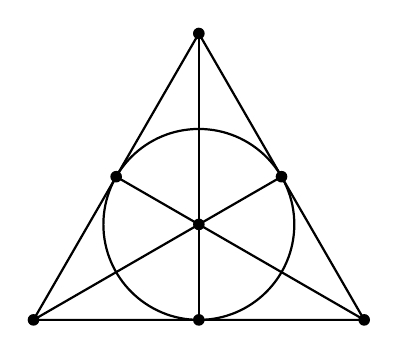
\begin{tikzpicture}[scale=0.7,line width=0.8pt]

  % --- Coordinates ---
  % Triangle vertices
  \coordinate (A) at (3,5.196);   % top
  \coordinate (B) at (0,0);       % bottom left
  \coordinate (C) at (6,0);       % bottom right
  % Edge midpoints
  \coordinate (F) at (1.5,2.598); % left edge midpoint
  \coordinate (D) at (4.5,2.598); % right edge midpoint
  \coordinate (E) at (3,0);       % bottom edge midpoint
  % Center (centroid / incenter)
  \coordinate (O) at (3,1.732);

  % --- The 7 lines ---
  % 3 sides of the triangle
  \draw (A) -- (B) -- (C) -- cycle;
  % 3 medians (vertex to opposite midpoint, through center)
  \draw (A) -- (E);
  \draw (B) -- (D);
  \draw (C) -- (F);
  % 7th line: the incircle through the three edge midpoints
  \draw (O) circle (1.732);

  % --- The 7 points ---
  \foreach \p in {A,B,C,D,E,F,O}
    \fill (\p) circle (3pt);

\end{tikzpicture}
\end{center}
Now, we observe that every $g\in G$ acts by conjugation on the set of points and lines, and preserves the incidence relation, with only the identity element in $G$ that fixes all the points. Therefore, $G$ is isomorphic to a subgroup of $\aut\left( \mathcal{F} \right)$. Any automorphism of $\mathcal{F}$ that fixes any two points on a line and fixes a third point not on the line will necessarily fix all points, meaning that any automorphism of $\mathcal{F}$ is determined by its action on any three non-collinear points. There are $168$ such triples, so $\mathcal{F}$ has at most $168$ automorphisms, so that if the simple group $G$ exists, then it is unique and isomorphic to $\aut\left( \mathcal{F} \right)$.

To determine the automorphisms of $\mathcal{F}$, we consider a different construction. Let $V = \F_2^{3}$ be the $3$-dimensional vector space over $\F_2$. Call the $7$ $1$-dimensional subspaces of $V$ the points and the $7$ $2$-dimensional subspaces the lines. Say a point is incident to a line via subspace inclusion. Observe that $\GL\left( V \right)$ acts faithfully on the points and lines and preserves incidence, so $\aut\left( \mathcal{F} \right)$ has order at least $168$, so $\aut\left( \mathcal{F} \right)\cong \GL\left( V \right) = \GL_3\left( \F_2 \right)$, with $\aut\left( \mathcal{F} \right)$ having order $168$.

Finally, we will prove that $\GL\left( V \right)$ is simple. Suppose $H$ is a proper nontrivial normal subgroup of $\GL\left( V \right)$. Suppose $\Omega$ is the set of points, and $N$ is the stabilizer in $\GL\left( V \right)$ of a point in $\Omega$. The intersection of all the conjugates of $N$ fixes all points, so this intersection is the identity. Therefore, $H\nleq N$, and we have $\GL\left( V \right) = HN$.

By the second isomorphism theorem, $\left[ H:H\cap N \right] = \left[ HN:N \right]$, so $7$ divides $\left\vert H \right\vert$. Furthermore, since $\GL(V)$ is isomorphic to a subgroup of $S_7$ and the normalizers of $7$-Sylow subgroups of $S_7$ have order $42$, it follows that $\GL(V)$ does not have a normal $7$-Sylow subgroup, so $n_7\left( \GL\left( V \right) \right) = 8$. 

A normal $7$-Sylow subgroup of $H$ is characteristic in $H$, hence normal in $\GL(V)$, meaning that $H$ does not have a unique $7$-Sylow subgroup. Since $n_7(H)\equiv 1$ mod $7$, and $n_7(H)\leq n_7\left( \GL(V) \right) = 8$, it follows that $n_7(H) = 8$. Thus, $\left\vert H \right\vert$ is divisible by $8$, so $56$ divides $H$, and since $H$ is proper, $\left\vert H \right\vert = 56$. By applying a Sylow-style counting argument to $H$, we see that $H$ has a normal (hence characteristic) $2$-Sylow subgroup, which is thus normal in $\GL(V)$. Yet, this would mean that $\GL(V)$ has a unique $2$-Sylow subgroup. Note that the upper and lower triangular matrices are subgroups of $\GL_3\left( \F_2 \right)$ with order $8$, so we achieve a contradiction.
\section{Ring Theory and Module Theory}%
\subsection{Ring Theory Notes}%
\subsubsection{Localization}%
If $R$ is a (commutative, unital) ring, then we may consider a subset $S\subseteq R$ such that $1\in S$, $0\notin S$, and for any $s_1,s_2\in S$, we have $s_1s_2\in S$ (such an $S$ is called a \textit{multiplicative set}). Then, we may construct the \textit{ring of fractions} $S^{-1}R$ as the set of equivalence classes in $R\times S$ with $\left( r_1,s_1 \right)\sim \left( r_2,s_2 \right) $ if and only if there exists $t\in S$ such that $ t\left( r_1s_2 - r_2s_1 \right) = 0$. We write $\left[ \left( r,s \right) \right] = \frac{r}{s}$, and define addition and multiplication by
\begin{align*}
  \frac{r_1}{s_1} + \frac{r_2}{s_2} &= \frac{r_1s_2 + r_2s_1}{s_1s_2}\\
  \frac{r_1}{s_1}\frac{r_2}{s_2} &= \frac{r_1r_2}{s_1s_2}.
\end{align*}
There is a natural embedding $\iota$ of $R$ into $S^{-1}R$ by taking $r\mapsto \frac{r}{1}$. 
\begin{theorem}
  Let $R$ be a commutative ring with unity, $S$ a multiplicatively closed subset, and $\phi\colon R\rightarrow T$ a ring homomorphism that maps $S$ to units in $T$. Then, there is a unique homomorphism $\varphi\colon S^{-1}R\rightarrow T$ such that $\varphi\circ\iota = \phi$.
  \begin{center}
    % https://tikzcd.yichuanshen.de/#N4Igdg9gJgpgziAXAbVABwnAlgFyxMJZABgBpiBdUkANwEMAbAVxiRACUQBfU9TXfIRQBGclVqMWbAMoA9YAFphXTjz7Y8BIqOHj6zVohAAVbuJhQA5vCKgAZgCcIAWyRkQOCEgBM1fVKMAHUC0AAssEGoGOgAjGAYABX5NIRAHLEtQnG5eEEcXN2pPJFEJAzZg-Bw6HPsnV0RS4sRfMoCQYPoHMIiuCi4gA
    \begin{tikzcd}
    R \arrow[rd, "\phi"'] \arrow[r, "\iota"] & S^{-1}R \arrow[d, "\varphi"] \\
                                             & T                           
    \end{tikzcd}
  \end{center}
\end{theorem}
\begin{proof}
  Define
  \begin{align*}
    \varphi\left( \frac{r}{s} \right) &= \phi\left( r \right)\phi\left( s \right)^{-1}.
  \end{align*}
\end{proof}
\begin{proposition}
  Let $R$ be a commutative ring with identity. Any ideal in $S^{-1}R$ is of the form $S^{-1}J$ for some ideal $J$ of $R$.
\end{proposition}
\begin{proof}
  Consider a proper ideal $I$ of $S^{-1}R$, and let $J = I\cap R$. We claim that $J\cap S = \emptyset$. If not, let $u\in J\cap S$, so that $\frac{u}{1}\in J\cap S$. Since $J\cap S$ is an ideal, it follows that $\frac{u}{1}\frac{1}{u}\in J\cap S$, so $1\in J\cap S$, so $1\in J$, so $1\in I$, meaning $I$ is not proper.

  Since $J\cap S = \emptyset$, it follows that $S^{-1}J$ is well-defined. We will start by showing that $I\subseteq S^{-1}J$. Consider an element $\frac{a}{b}\in I$. Then, $\frac{a}{1} = \frac{a}{b}\frac{b}{1}$, so $\frac{a}{b}\in S^{-1}J$. Additionally, if $\frac{a}{b}\in S^{-1}J$, then $\frac{a}{b} = \frac{1}{b}\frac{a}{1}$, so since $\frac{a}{1}\in I$ as $\frac{a}{1}\in I\cap R$, it follows that $\frac{a}{b}\in I$.
\end{proof}
\begin{proposition}
  There is a one-to-one correspondence between prime ideals of $S^{-1}R$ and prime ideals of $R$ that do not intersect $S$.
\end{proposition}
\begin{proof}
  Let $\iota\colon R\rightarrow S^{-1}R$ be the embedding $r\mapsto \frac{r}{1}$. We claim that the maps
  \begin{align*}
    \mathfrak{p}&\mapsto S^{-1} \mathfrak{p}\\
    \mathfrak{q} &\mapsto \iota^{-1}\left( \mathfrak{q} \right)
  \end{align*}
  are mutually inverse.

  First, we observe that for any ideal $I\subseteq S^{-1}R$, then
  \begin{align*}
    \iota^{-1}\left( S^{-1}I \right) &= \set{r\in R : sr\in I\text{ for some }s\in S},
  \end{align*}
  known as the \textit{saturation} of the ideal $I\subseteq R$. This follows from the fact that if $sr\in I$, then $\frac{r}{1} = \frac{sr}{s}\in S^{-1}I$, meaning that $r\in \iota^{-1}\left( S^{-1}I \right)$, and if $\frac{r}{1} = \frac{a}{s}$ for some $a\in I$ and $s\in S$, then there is some $t\in S$ such that $t\left( rs-a \right) = 0$, so that $\left( ts \right)r = ta\in I$. Since $ts\in S$, it follows that $r$ belongs in the right-hand set.

  Next, we observe that $S^{-1}I = S^{-1}R$ if and only if $I\cap S \neq \emptyset$. This follows from the fact that if $s\in I\cap S$, then $\frac{s}{s} = \frac{1}{1}\in S^{-1}I$, while if $\frac{1}{1}\in S^{-1}I$, then we may write $\frac{1}{1} = \frac{a}{s}$ for some $a\in I$ and $s\in S$, with $t\left( s-a \right) = 0$, so $ts = ta\in I$, whence $ts\in I\cap S$.

  First, we show that the map $ \mathfrak{q}\mapsto \iota^{-1}\left( \mathfrak{q} \right) $ sends primes in $S^{-1}R$ to primes in $R$. Set $ \mathfrak{p} = \iota^{-1}\left( \mathfrak{q} \right) $. This follows from the fact that the primage of a prime under a ring homomorphism is still prime.

  Next, we show that if $ \mathfrak{p} $ is prime with $ \mathfrak{p}\cap S = \emptyset $, then $ S^{-1} \mathfrak{p} $ is prime. First, observe that
  \begin{align*}
    \iota^{-1}\left( S^{-1} \mathfrak{p} \right) &= \set{r\in R : sr\in \mathfrak{p}\text{ for some }s\in S}.
  \end{align*}
  Notice that whenever $sr\in \mathfrak{p}$ with $s\in S$, we must have $r\in \mathfrak{p}$. Therefore, we must have $\iota^{-1}\left( S^{-1} \mathfrak{p} \right) = \mathfrak{p}$.

  Next, $S^{-1} \mathfrak{p}$ is proper since $ \mathfrak{p}\cap S = \emptyset $. Finally, we will show that $S^{-1} \mathfrak{p}$ is prime.

  Suppose
  \begin{align*}
    \frac{a}{s}\frac{b}{t} &\in S^{-1} \mathfrak{p}
  \end{align*}
  with $a,b\in R$ and $s,t\in S$. Then, we have $\frac{ab}{st} = \frac{p}{u}$ for some $p\in \mathfrak{p}$ and $u\in S$. There is thus $w\in S$ such that $w\left( uab - stp \right) = 0$, giving $\left( wu \right)\left( ab \right) = wstp\in \mathfrak{p}$. Since $wu\in S$ is disjoint from $ \mathfrak{p} $, it follows that $wu\notin \mathfrak{p}$, and we have $ab\in \mathfrak{p}$. Therefore, $a\in \mathfrak{p}$ or $b\in \mathfrak{p}$, so $\frac{a}{s}\in S^{-1} \mathfrak{p}$ or $\frac{b}{t}\in S^{-1} \mathfrak{p}$.

  This gives the correspondence obtained by taking $ \mathfrak{p}\mapsto S^{-1} \mathfrak{p} $ and $ \mathfrak{q}\mapsto \iota^{-1}\left( \mathfrak{q} \right) $.
\end{proof}
We start by discussing a special case of localization.

Consider the special case of the multiplicative set $S = \set{1,r,r^2,\dots}$. We will show that $S^{-1}R \cong R[x]/\left( rx-1 \right)$, which will emerge by showing that $R[x]/\left( rx-1 \right)$ satisfies the universal property. That is, if $\varphi\colon R\rightarrow A$ is a ring homomorphism with $\varphi\left( 1 \right) = 1$ and $\varphi(S)\subseteq A^{\times}$, then there exists a unique ring homomorphism $ \Phi\colon R[x]/\left( rx-1 \right) \rightarrow A $ such that $\Phi\circ \ve = \varphi$, where $\ve$ is the composition
\begin{align*}
  R\xrightarrow{\iota} R[x] \xrightarrow{\pi} R[x]/\left( rx-1 \right).
\end{align*}
We start by setting $s = \varphi(r)^{-1}$, and extending $\varphi$ to a map $ \overline{\varphi}\colon R[x]\rightarrow A $ given by
\begin{align*}
  \overline{\varphi}\left( a_0 + a_1 x + \cdots + a_nx^{n} \right) &= \varphi\left( a_0 \right) + \varphi\left( a_1 \right)s + \cdots + \varphi\left( a_n \right)s^{n}.
\end{align*}
To define $ \Phi $, it suffices to show that $\left( rx-1 \right)\subseteq \ker\left( \overline{\varphi} \right)$. This follows from the fact that
\begin{align*}
  \overline{\varphi}\left( rx-1 \right) &= \varphi\left( r \right)s-1\\
                                        &= 0.
\end{align*}
Therefore, we have existence.

Now, suppose we have a homomorphism $\psi\colon R[x]/\left( rx-1 \right)\rightarrow A$ such that $ \psi\circ\ve = \varphi $ on $R$. We will show that $\psi\left( x + \left( rx-1 \right) \right) = \Phi\left( x + \left( rx-1 \right) \right)$, as we already know that $\psi\left( t + \left( rx-1 \right) \right) = \varphi(t) = \Phi\left( t + \left( rx-1 \right) \right)$ for any $t\in R$. Observing that $rx\equiv 1$ mod $\left( rx-1 \right)$, we have
\begin{align*}
  \psi\left( rx + \left( rx-1 \right) \right) &= \psi\left( 1 + \left( rx-1 \right) \right)\\
                                              &= 1,
\end{align*}
while
\begin{align*}
  \psi\left( rx + \left( rx-1 \right) \right) &= \psi\left( r + \left( rx-1 \right) \right) \psi\left( x + \left( rx-1 \right) \right)\\
                                              &= \varphi\left( r \right) \psi\left( x + \left( rx-1 \right) \right).
\end{align*}
Therefore, $\varphi\left( r \right) \psi\left( x + \left( rx-1 \right) \right) = 1$, so that $\psi\left( x + \left( rx-1 \right) \right) = \varphi\left( r \right)^{-1} = \Phi\left( x + \left( rx-1 \right) \right)$.
\subsubsection{Unique Factorization Domains}%
\begin{definition}
  An integral domain $R$ is called a \textit{unique factorization domain} if every element $r\in R$ that is nonzero and non-unit admits a factorization
  \begin{align*}
    r &= up_1^{e_1}\cdots p_n^{e_n}
  \end{align*}
  into irreducible elements of $R$. The factorization is unique up to associates, where $q\sim p$ are associates if there exists $v\in R^{\times}$ such that $q = vp$.
\end{definition}
A general strategy with unique factorization domains consists of writing any nonzero non-units in terms of their irreducibles, and using divisibility to tease out properties. An example is discussed in the following.
\begin{example}[August `21, Problem 4]
  Consider a nonzero non-unit $up_1^{d_1}\cdots p_m^{d_m} = f\in R$ in a unique factorization domain. Let $R_f = R\left[ \frac{1}{f} \right]$. We will show that
  \begin{align*}
    R_f^{\times} &= \set{up_1^{e_1}\cdots p_m^{e_m} : u\in R^{\times}, e_i\in \Z}.
  \end{align*}
  To show one direction, observe that we may obtain any individual factor $p_i$ of $f$ by taking
  \begin{align*}
    p_i &= \frac{f}{up_1^{d_1}\cdots p_i^{d_{i}-1}\cdots p_m^{d_m}},
  \end{align*}
  so in the localization, we have all positive powers of $p_i^{d_i}$ are invertible in $R_f$, as well as all negative powers since
  \begin{align*}
    \frac{1}{p_i} &= \frac{up_1^{d_1}\cdots p_i^{d_{i}-1}\cdots p_m^{d_m}}{f},
  \end{align*}
  so that the latter set is contained in the former. Meanwhile, if $\frac{s}{f^{n_1}}\in R_f^{\times}$, then we use the fact that the factorization of $f$ is unique to find that $\frac{s}{u}\left( p_1^{-d_1}\cdots p_m^{-d_m} \right) = su^{-1}\left( p_1^{-d_1}\cdots p_m^{-d_m} \right)$ is contained in the latter set.

  This allows us to develop an isomorphism $R_f^{\times}\cong R^{\times}\times \Z^{m}$, where we take any unit in $R_f^{\times}$ to the tuple $\left( u,e_1,\dots,e_m \right)$.
\end{example}
\subsubsection{Primality in the Gaussian Integers}%
We will discuss primality in the Gaussian integers. Recall that the Gaussian integers are given by
\begin{align*}
  \Z\left[ i \right] &= \set{a + bi | a,b\in \Z}\\
                     &\cong \frac{\Z\left[ x \right]}{\left( x^2 + 1 \right)}.
\end{align*}
The Gaussian integers are equipped with a norm $N\colon \Z\left[ i \right]\rightarrow \Z_{\geq 0}$ given by $N\left( a+bi \right) = \left( a+bi \right)\left( a-bi \right) = a^2 + b^2$, which is a multiplicative norm satisfying $N\left( zw \right) = N\left( z \right)N\left( w \right)$. Furthermore, with this norm, the Gaussian integers form a Euclidean domain. The units of $\Z\left[ i \right]$ are $\pm 1$ and $\pm i$.
\begin{lemma}
  Let $q\in \Z\left[ i \right]$. Then, there is a prime integer $p\in \Z$ such that $N\left( q \right) = p$ or $N\left( q \right) = p^2$.
\end{lemma}
\begin{proof}
  Since $q$ is not a unit, $N\left( q \right)\neq 1$. Therefore, $N\left( q \right)$ is a nontrivial product of prime integers, and since $q$ is prime in $\Z\left[ i \right]$, $q$ must divide one of the prime integer factors of $N\left( q \right)$. Let $p$ be this prime integer.

  Then, $q | p$ in $\Z\left[ i \right]$, so $N\left( q \right) | N\left( p \right) = p^2$, so $N\left( q \right) = p$ or $N\left( q \right) = p^2$.
\end{proof}
\begin{example}
  We observe that $3$ is a prime element of $\Z\left[ i \right]$. Since $\Z\left[ i \right]$ is a Euclidean domain, it is a UFD, so irreducibles are prime, meaning we only need to show that $3$ is irreducible in $\Z\left[ i \right]$.

  Since $N\left( 3 \right) = 9$, it follows that the norm of any factor of $3$ must be a divisor of $9$. Therefore, it follows that the norm of any divisor of $3$ is equal to $1$, $3$, or $9$. If the norm is $9$, then the factor is an associate of $3$, while if the norm is $1$, then the factor is a unit, so it follows that any nontrivial factor of $3$ would have norm equal to $3$. Yet, there are no such elements.

  Meanwhile, $5$ is not a prime element of $\Z\left[ i \right]$, since we may write $5 = \left( 2+i \right)\left( 2-i \right)$.
\end{example}
We will now focus on proving one of the most celebrated theorems in number theory: Fermat's Theorem on sums of squares. We will say a prime integer $p\in \Z$ \textit{splits} in $\Z\left[ i \right]$ if it is not a prime element of $\Z\left[ i \right]$. For example, $5$ splits in $\Z\left[ i \right]$ while $3$ does not.
\begin{lemma}
  A positive prime integer $p\in \Z$ splits in $\Z\left[ i \right]$ if and only if it is the sum of two squares in $\Z$.
\end{lemma}
\begin{proof}
  Suppose $p = a^2 + b^2$ with $a,b\in \Z$. Then,
  \begin{align*}
    p = \left( a+bi \right)\left( a-bi \right)
  \end{align*}
  in $\Z\left[ i \right]$, so since $N\left( a\pm bi \right) = a^2 + b^2 = p \neq 1$, it follows that neither of the factors is a unit in $\Z\left[ i \right]$, so that $p$ is not irreducible, hence not prime.

  Conversely, suppose $p$ is not irreducible in $\Z\left[ i \right]$. Then, $p$ has an irreducible factor $q\in \Z\left[ i \right]$ that is not an associate of $p$. Since $q | p$, multiplicativity of the norm gives that $N\left( q \right) | N\left( p \right) = p^2$, hence $N\left( q \right) = p $ as $q$ and $p$ are not associates and $q$ is not a unit. If we have $q = a + bi$, then
  \begin{align*}
    p &= N\left( q \right)\\
      &= a^2 + b^2.
  \end{align*}
\end{proof}
Next, we discuss a characterization of splitting via a single congruence. 
\begin{lemma}
  A positive odd prime integer $p$ splits in $\Z\left[ i \right]$ if and only if it is congruent to $1$ modulo $4$.
\end{lemma}
\begin{proof}
  Our goal is to understand when $\Z\left[ i \right]/\left( p \right)$ is an integral domain. Yet, we have the series of isomorphisms
  \begin{align*}
    \frac{\Z\left[ i \right]}{\left( p \right)} &\cong \frac{\Z\left[ x \right]/\left( x^2 + 1 \right)}{\left( p \right)}\\
                                                &\cong \frac{\Z\left[ x \right]}{\left( p,x^2 + 1 \right)}\\
                                                &\cong \frac{\Z\left[ x \right]/\left( p \right)}{\left( x^2 + 1 \right)}\\
                                                &\cong \frac{\Z/p\Z\left[ x \right]}{\left( x^2 + 1 \right)}.
  \end{align*}
  In particular, this means that $p$ splits in $\Z\left[ i \right]$ if and only if $x^2 + 1$ has a root in $\Z/p\Z$, or that there is some $n$ such that $n^2\equiv -1$ modulo $p$. We will show that this condition is equivalent to $p$ being congruent to $1$ modulo $4$.

  Let $G = \left( \Z/p\Z \right)^{\times}$, and fix a generator $g$. Observe that $p$ is odd, so $p-1 = 2\ell$ for some integer $\ell$. Let $ \overline{n} $ denote the class of an integer $n$ mod $\left( p \right)$. For any $n\notin \left( p \right)$, it follows that there is some $m$ such that $ \overline{n} = g^{m} $.

  Observe that the class $ \overline{-1} $ generates the unique subgroup of order $2$ of $G$, and since $g^{\ell}$ does the same, it follows that $g^{\ell} = -1$. In particular, we have that $n^2 = -1$ modulo $p$ if and only if $g^{2m} = g^{\ell}$, or that $2m\equiv \ell$ mod $2\ell$, or that $\left( p-1 \right) = 2\ell$ is a multiple of $4$, or $p\equiv 1$ mod $4$.
\end{proof}
This gives the following.
\begin{theorem}[Fermat's Theorem on Sums of Squares]
  A positive odd prime $p\in \Z$ is a sum of two squares if and only if $p\equiv 1$ mod $4$.
\end{theorem}
As a general technique for primality in a quadratic number ring $\Z\left[ \sqrt{d} \right]$ for some square-free integer $d$, we use the fact that
\begin{align*}
  \Z\left[ \sqrt{d} \right] &\cong \frac{\Z\left[ x \right]}{\left( x^2-d \right)},
\end{align*}
meaning that an element $p\in \Z$ is prime if and only if
\begin{align*}
  \frac{\Z\left[ \sqrt{d} \right]}{\left( p \right)} &\cong \frac{\Z\left[ x \right]}{\left( p,x^2-d \right)}\\
                                                     &\cong \frac{\left( \Z/p\Z \right)\left[ x \right]}{\left( x^2-d \right)}
\end{align*}
is an integral domain; equivalently, we want to see whether or not $x^2-d$ is irreducible mod $p$.
\subsection{Module Theory: Useful Facts}%
\begin{definition}
  A module $M$ over $R$ is called \textit{cyclic} if there is a vector $v$ such that $ \left\langle v \right\rangle = Rv = M $.
\end{definition}
\begin{theorem}
  If a module $M$ is cyclic with cyclic vector $v$, then
  \begin{align*}
    M &\cong R/\operatorname{Ann}_R(v),
  \end{align*}
  where $\operatorname{Ann}_R(v)$ is the \textit{annihilator ideal}, defined by
  \begin{align*}
    \operatorname{Ann}_R(v) &= \set{r\in R : rv = 0}.
  \end{align*}
\end{theorem}
What follows are the most important theorems in module theory. We'll discuss an application of it to linear algebra.
\begin{definition}
  Let $R$ be a PID. A matrix $A\in \Mat_{k,n}\left( R \right)$ is said to be in Smith Normal Form if there exists $m\leq \min\left( k,n \right)$ and nonzero elements $d_1,\dots,d_m$ such that $A = \operatorname{diag}_{k,n}\left( d_1,\dots,d_m \right)$ satisfying $\left( d_1 \right)\supseteq \left( d_2 \right)\supseteq\cdots\supseteq \left( d_m \right)$.
\end{definition}
\begin{theorem}[Smith Normal Form Decomposition]
  Let $R$ be a PID, and let $A\in \Mat_{k,n}\left( R \right)$. Then, there are $U\in \GL_k\left( R \right)$ and $V\in \GL_n\left( R \right)$ such that $UAV$ is in Smith Normal Form.
\end{theorem}
These matrices are found by a product of elementary row and column operations. Specifically, the following row operations can be interpreted by matrix multiplication, where $E_{ij}(\lambda)$ denotes the elementary matrix consisting of $1$ along the diagonal and $\lambda$ at the $(i,j)$ position, while $F_{ij}$ denotes the transposition matrix with row $i$ and row $j$ exchanged.
\begin{center}
  \begin{tabular}{c|c}
    Elementary Row Operation & Interpretation as Matrix Multiplication\\
    \hline
    $R_i(A)\mapsto R_i(A) + \lambda R_j(A)$ & $A\mapsto E_{ij}(\lambda)A$\\
    $C_i(A)\mapsto C_i(A) + \lambda C_j(A)$ & $A\mapsto AE_{ij}(\lambda)$\\
    $R_i(A)\leftrightarrow R_j(A)$ & $A\mapsto F_{ij} A$\\
    $C_i(A)\leftrightarrow C_j(A)$ & $A\mapsto AF_{ij}$
  \end{tabular}
\end{center}

\begin{theorem}[Compatible Basis Theorem]
  Let $M$ be a rank $n$ free module over a principal ideal domain $R$, and let $N$ be a submodule of $M$. Then, $N$ is a free module with rank $m\leq n$, and there is a basis $\set{y_1,\dots,y_n}$ for $M$ and nonzero non-units $d_1 | d_2 | \cdots | d_m$ such that $\set{d_1y_1,d_2y_2,\dots,d_my_m}$.

  Moreover, the rank $m$ of $N$ is unique, and the $d_1,\dots,d_m$ are unique up to associates.
\end{theorem}
\begin{proof}
  Select a basis $\set{x_1,\dots,x_n}$ for $M$, and a set of generators $\set{u_1,\dots,u_k}$ of $N$. Then, we may find a matrix $\left( a_{ij} \right)_{i,j}\in \Mat_{k,n}\left( R \right)$ such that
  \begin{align*}
    \begin{pmatrix}u_1\\\vdots\\u_k\end{pmatrix} &= \left( a_{ij} \right)_{i,j} \begin{pmatrix}x_1\\\vdots\\x_n\end{pmatrix}.
  \end{align*}
  We may put the matrix $A$ into Smith normal form, yielding $A = PDQ$, where $D = \operatorname{diag}_{k,n}\left( d_1,\dots,d_m \right)$, $P\in \GL_k\left( R \right)$, and $Q\in \GL_n\left( R \right)$.

  Writing
  \begin{align*}
    \begin{pmatrix}y_1\\\vdots\\y_n\end{pmatrix} &= Q \begin{pmatrix}x_1\\\vdots\\x_n\end{pmatrix}\\
    \begin{pmatrix}v_1\\\vdots\\v_k\end{pmatrix} &= P^{-1} \begin{pmatrix}u_1\\\vdots\\u_k\end{pmatrix},
  \end{align*}
  we have that $\set{y_1,\dots,y_n}$ are a basis for $M$ and $\set{v_1,\dots,v_k}$ generate $N$. We may write
  \begin{align*}
    \begin{pmatrix}v_1\\\vdots\\v_k\end{pmatrix} &= D \begin{pmatrix}y_1\\\vdots\\y_n\end{pmatrix},
  \end{align*}
  meaning that $k = m$ and $v_i = d_iy_i$.
\end{proof}
\begin{theorem}[Invariant Factors Decomposition]
  Let $M$ be a finitely generated module over a PID $R$. Then, there exists a unique $k$, unique $\ell$, and unique up to associates $a_1 | a_2 | \cdots | a_{\ell}$ such that
  \begin{align*}
    M &\cong R^{k}\oplus \left( \bigoplus_{i=1}^{\ell} R/\left( a_i \right) \right).
  \end{align*}
\end{theorem}
\begin{proof}[Proof Sketch]
  If $\set{x_1,\dots,x_n}$ forms a generating set for $M$, define a (surjective) $R$-module homomorphism $R^{n} = F\rightarrow M$ by taking $\left( r_1,\dots,r_n \right)\mapsto \sum_{i=1}^{n}r_ix_i$. Find a compatible basis for $F$ and the kernel $N\leq F$ of this homomorphism. Then, we get that
  \begin{align*}
    M &\cong F/N\\
      &= \frac{\bigoplus_{i=1}^{n}Ry_i}{\bigoplus_{i=1}^{m}\left( a_i \right)y_i}\\
      &\cong R^{n-m} \oplus \left( \bigoplus_{i=1}^{m}R/\left( a_i \right) \right).
  \end{align*}
\end{proof}
\begin{theorem}[Elementary Divisors Decomposition]
  Let $M$ be a finitely generated module over a PID $R$. Then, there are primes $p_1,\dots,p_t\in R$ not necessarily unique and $d_1,\dots,d_t\in \N$ such that
  \begin{align*}
    M &\cong R^{k}\oplus \left( \bigoplus_{i=1}^{t}R/\left( p_i^{d_i} \right) \right).
  \end{align*}
  Here, $k$ is the same value as the $k$ in the invariant factors decomposition.
\end{theorem}
\begin{proof}[Proof Sketch]
  Since $R$ is a principal ideal domain, it is a unique factorization domain, so for each $a_i$ in the invariant factors decomposition, we may write $a_i = p_{i,1}^{d_1}\cdots p_{i,t}^{d_t}$. The Chinese Remainder Theorem yields that
  \begin{align*}
    R/\left( a_i \right) &\cong \bigoplus_{s=1}^{t} R/\left( p_{i,s}^{d_{s}} \right).
  \end{align*}
\end{proof}
\begin{definition}
A module $P$ over a (commutative, unital) ring $R$ is called \textit{projective} if it satisfies the following criterion: given a surjective $R$-module homomorphism $\varphi\colon M\rightarrow N$, any $R$-module homomorphism $\psi\colon P\rightarrow N$ extends to an $R$-module homomorphism $ \widetilde{\psi}\colon P\rightarrow M $ satisfying $\varphi\circ \widetilde{\psi} = \psi$. The following diagram commutes.
\begin{center}
  % https://tikzcd.yichuanshen.de/#N4Igdg9gJgpgziAXAbVABwnAlgFyxMJZABgBoBGAXVJADcBDAGwFcYkQBZEAX1PU1z5CKchWp0mrdgDkefEBmx4CRAExiaDFm0Qhic-kqFFRxcVqm6ACj3EwoAc3hFQAMwBOEALZIAzDRwIJDIQRiwwHRAoejgAC3sQGkZ6ACMYRisBZWEQdywHWJxEiW12AB0ymAAPLDgcOAACCoB3LFg8RlhgCrRsbgMQD28-AKDEURLLEB7sAaGfRBDApAnktIys4108gqLNSUiKhnc0WKw5zwWJ5cRVbkpuIA
\begin{tikzcd}
                        & P \arrow[ld, "\exists \widetilde{\psi}"', dashed] \arrow[d, "\psi"] &   \\
M \arrow[r, "\varphi"'] & N \arrow[r]                                                         & 0
\end{tikzcd}
\end{center}
\end{definition}
\subsubsection{Tensor Products}%
\begin{definition}
  Let $R$ be any ring. If $M$ is a \textit{right} $R$-module, $N$ is a left $R$-module, and $P$ is an abelian group, a map $\varphi\colon M\times N\rightarrow P$ is called \textit{$R$-balanced} if
  \begin{align*}
    \varphi\left( m_1 + m_2,n \right) &= \varphi\left( m_1,n \right) + \varphi\left( m_2,n \right)\\
    \varphi\left( m,n_1 + n_2 \right) &= \varphi\left( m,n_1 \right) + \varphi\left( m,n_2 \right)\\
    \varphi\left( mr,n \right) &= \varphi\left( m,rn \right)
  \end{align*}
  for all $m,m_1,m_2\in M$, $n,n_1,n_2\in N$, and $r\in R$.

  If $R$ is commutative, (i.e., both $M$ and $N$ can be considered as left $R$-modules) then the map $\varphi$ is called \textit{$R$-bilinear} if we also have $\varphi\left( rm,n \right) = r\varphi\left( m,n \right) = \varphi\left( m,rn \right)$.
\end{definition}
\begin{definition}
  Let $R$ be any ring. If $M$ and $N$ are a right $R$-module and left $R$-module respectively, their \textit{tensor product} is the unique abelian group satisfying the following universal property: for any $R$-balanced map $\phi\colon M\times N\rightarrow P$, there is a unique abelian group homomorphism $\varphi\colon M\otimes_{R}N\rightarrow P$ satisfying $\varphi\left( m\otimes n \right) = \phi\left( m,n \right)$.

  If $R$ is a commutative ring (i.e., left and right $R$-modules are the same), then $M\otimes_{R}N$ satisfies the following stronger universal property: for any $R$-bilinear map $\phi\colon M\times N\rightarrow P$ of left $R$-modules, there is a unique $R$-module homomorphism $\varphi\colon M\otimes_{R}N\rightarrow P$, where $M\otimes_{R}N$ is endowed with the $R$-module structure given by $r\left( m\otimes n \right)= \left( rm \right)\otimes n = m\otimes \left( rn \right)$.
\end{definition}
A very useful case study is the \textit{extension of scalars}. Given an inclusion of unital rings $R\rightarrow S$, there is a natural right $R$-module structure on $S$ given by left multiplication; taking the left multiplication by $S$ yields a $\left( S,R \right)$-bimodule structure on the ring $S$. If $N$ is a left $R$-module, then $S\otimes_{R}N$ becomes a left $S$-module with a copy of $N$ included via the map $\iota\colon N\rightarrow S\otimes_{R}N$ taking $n\mapsto 1\otimes n$.

If $f\colon R\rightarrow S$ is a unital ring homomorphism, then $S$ receives the structure of a right $R$-module by taking $s\cdot r = sf\left( r \right)$, and $S$ becomes a $\left( S,R \right)$-bimodule with respect to the standard left $S$-module structure and the described right $R$-module structure. The tensor product $S\otimes_{R}N$ of any left $R$-module with $S$ yields a \textit{change of base} from the ring $R$ to the ring $S$.

Finally, if $I$ is a two-sided ideal of a (not necessarily commutative) ring $R$, then $R/I$ is a $\left( R/I,R \right)$-bimodule; given a left $R$-module $N$, then $R/I\otimes_{R}N$ becomes a left $R/I$-module (i.e., the change of base with respect to the quotient homomorphism). Defining
\begin{align*}
  IN &= \set{\sum_{i=1}^{n}a_in_i : a_i\in I, n_i\in N},
\end{align*}
we obtain that $IN$ is a left $R$-submodule of $N$.

The tensor product $\left( R/I \right)\otimes_{R}N$ is generated by the simple tensors $\left( r+I \right)\otimes n = r\left( \left( 1 + I \right)\otimes n \right)$ for any $r\in R$ and $n\in N$. Therefore, the elements $\left( 1+I \right)\otimes n$ generate $\left( R/I \right)\otimes_{R}N$ as an $R/I$-module. Define the map $N\rightarrow \left( R/I \right)\otimes_{R}N$ by taking $n\mapsto \left( 1+I \right)\otimes n$. This is a surjective left $R$-module homomorphism with kernel containing $IN$, seeing as if $a\in I$ and $n\in N$, then $\left( 1+I \right)\otimes an = \left( a + I \right)\otimes n = 0$. We obtain a surjective $R$-module homomorphism $f\colon N/IN\rightarrow \left( R/I \right)\otimes_{R}N$ taking $n + IN\mapsto \left( 1+I \right)\otimes n$. Define an inverse $R$-balanced map $R/I\times N\rightarrow N/IN$ taking $\left( r + I,n \right)\mapsto rn + IN$. Using the universal property yields the following standard isomorphism:
\begin{align*}
  R/I\otimes_{R}N &\cong N/IN.
\end{align*}
\subsubsection{Nakayama's Lemma}%
\begin{definition}
  The \textit{Jacobson radical} $ \mathfrak{J} $ of a commutative ring $A$ is the intersection of all the maximal ideals.
\end{definition}
\begin{lemma}
  Let $x\in A$. The following are equivalent:
  \begin{enumerate}[(i)]
    \item $x\in \mathfrak{J} $;
    \item $1 + xy\in A^{\times}$ for all $y\in R$.
  \end{enumerate}
\end{lemma}
\begin{proof}
  Suppose $x\in \mathfrak{J}$. If it were the case that $1+ x\notin A^{\times}$, then $ \left( 1 + x \right)\neq A $, so it is contained in some maximal ideal $ \mathfrak{m} $ of $A$. Yet, that implies that $1$ is in the maximal ideal $ \mathfrak{m} $ since $x\in \mathfrak{m}$, implying that $ \mathfrak{m} = A $.

  Suppose $x\notin \mathfrak{m}$ for some maximal ideal $ \mathfrak{m} $ of $A$. Then, $ \mathfrak{m} + \left( x \right) = A $, so there is some $y\in A$ such that $1 + xy\in \mathfrak{m}$, implying that $1 + xy\notin A^{\times}$.
\end{proof}
\begin{lemma}
  Let $ \mathfrak{a} $ be an ideal of a commutative ring $A$ that is contained in the Jacobson radical $ \mathfrak{J} $. Let $E$ be a finitely generated $A$-module. Suppose $ \mathfrak{a}E = E $. Then, $E = \set{0}$.
\end{lemma}
\begin{proof}
  We induct on the number of generators of $E$. Let $x_1,\dots,x_s$ be generators of $E$. Then, there exist $a_1,\dots,a_s\in \mathfrak{a}$ such that
  \begin{align*}
    x_s &= a_1x_2 + \cdots + a_sx_s,
  \end{align*}
  meaning there is some $a\in \mathfrak{a}$ such that $\left( 1 + a \right)x_s\in \left\langle x_1,\dots,x_{s-1} \right\rangle$. Notice that $1 + a$ is a unit in $ A $ since $ \mathfrak{a}\subseteq \mathfrak{J}$. Therefore, $x_s\in \left\langle x_1,\dots,x_{s-1} \right\rangle$, so induction gives the desired result.
\end{proof}
\begin{lemma}
  If $A$ is a local ring, and $E$ is a finitely generated $A$-module with a submodule $F$, then if $E = F + \mathfrak{m}E$, we have $E = F$.
\end{lemma}
\begin{proof}
  Apply the previous lemma to the quotient ring $E/F$.
\end{proof}
\subsubsection{Jordan Canonical Form}%
If we are given a finite-dimensional vector space $V$ over a field $F$ and a linear transformation $T\colon V\rightarrow V$, then $V$ attains the structure of an $F[x]$-module by defining the action of $x$ by $x\cdot v = Tv$. In particular, this means that we may apply the invariant factors and elementary divisors decomposition(s) to $V$ to obtain different canonical forms of $T$. The application of the invariant factors decomposition yields the rational canonical form. It can be shown that the rational canonical form of $A\in \Mat_{n}\left( F \right)$ is computed by taking the Smith Normal Form of the matrix $xI - A$.

Here, we will focus on applying the elementary divisors decomposition (in the special case of an algebraically closed field) to obtain the Jordan Canonical Form. Then, we will discuss some applications of this. By the definition of the $F[x]$-module structure on $V$, the element $T$ acts on $V$ by $x$ acting by multiplication on each of the cyclic summands $F[x]/\left( x-\lambda \right)^{k}$.

Define an ordered basis
\begin{align*}
  \set{ \left( \overline{x}-\lambda \right)^{k-1}, \left( \overline{x}-\lambda \right)^{k-2},\dots, \overline{x}-\lambda, 1 }
\end{align*}
for the quotient $F[x]/\left( x-\lambda \right)^{k}$. Viewing $ \left( \overline{x}-\lambda \right)^{k} = 0 $ in the quotient, we have that $x$ acts as
\begin{align*}
  x\left( \overline{x}-\lambda \right)^{k-1} &= \lambda \left( \overline{x}-\lambda \right)^{k-1} + \left( \overline{x}-\lambda \right)^{k}\\
                                             &= \lambda \left( \overline{x}-\lambda \right)^{k-1}\\
  x\left( \overline{x}-\lambda \right)^{k-2} &= \lambda \left( \overline{x}-\lambda \right)^{k-2} + \left( \overline{x}-\lambda^{k-1} \right)\\
                                             &\vdots\\
  \overline{x}-\lambda &= \lambda \left( \overline{x}-\lambda \right) + \left( \overline{x}-\lambda \right)^{2}\\
  x &= \lambda(1) + \left( \overline{x}-\lambda \right).
\end{align*}
This yields the matrix
\begin{align*}
  \begin{pmatrix}\lambda & 1 & & & \\ & \lambda & \ddots & & \\ & & \ddots & 1 & \\ & & & \lambda & 1 \\ & & & & \lambda\end{pmatrix}.
\end{align*}
Each of the cyclic summands $F[x]/\left( x-\lambda \right)^{k}$ correspond to the \textit{generalized eigenspaces} of $T$ corresponding to the eigenvalue $\lambda$.

Notice that the minimal polynomial of a Jordan block $J_d(\lambda)$ is given by $\left( x-\lambda \right)^{d}$. In particular, if $\lambda = 0$, we have that $F[x]/x^{d}$ admits a minimal polynomial of $\mu(x) = x^d$.
\begin{theorem}
  The total number of Jordan blocks with eigenvalue $\lambda$ is given by the geometric multiplicity of $\lambda$. That is, the number of Jordan blocks with eigenvalue $\lambda$ is given by $\dim\ker\left( A-\lambda I \right)$.
\end{theorem}
Assume $\lambda\neq 0$. Considering the transformation corresponding to $T^2 = J_n(\lambda)^2$, we observe that we may write
\begin{align*}
  x^2-\lambda^2 &= \left( x-\lambda \right)\left( x+\lambda \right).
\end{align*}
In particular, this means that the minimal polynomial $\mu_{T^2}(y)$ divides $\left( y-\lambda \right)^{n}\left( y+\lambda \right)^{n}$. Since the greatest common divisor of $\left( x-\lambda \right)$ and $\left( x+\lambda \right)$ is $1$, we have that $\left( \overline{x}+\lambda \right)^{d}$ is invertible in $F[x]/\left( x-\lambda \right)^{n}$ for any exponent $d$; the minimal polynomial $\mu_{T^2}(y)$ of $T^2$ will thus divide $\left( y-\lambda^2 \right)^{n}$. Since $\left( \overline{x}^2-\lambda^2 \right)^{d} = \left( \overline{x}-\lambda \right)^{d} \theta$, where $\theta$ is some invertible element of $F[x]/\left( x-\lambda \right)^{n}$, it follows that $\left( \overline{x}^2-\lambda^2 \right)^{d} \neq 0$ for any $0\leq d < n$, meaning that the minimal polynomial $\mu_{T^2}$ of $T^2$ is equal to $\left( x-\lambda^2 \right)^{n}$.
\section{Representation Theory}%
We assume that the group $G$ is finite and that all representations are complex unless stated otherwise.
\begin{itemize}
  \item \textbf{Schur's Lemma:} If $M$ is a simple $R$-module, then $\operatorname{End}_{R}\left( M \right)$ is a division ring. Equivalently, if $M$ is a simple $\C$-module, then any element $T\in \operatorname{End}_{\C}\left( M \right)$ is a diagonal operator $T = \lambda I$.
  \item \textbf{Maschke's Theorem:} Suppose we are given a representation $\rho\colon G\rightarrow \GL_n(F)$ over an arbitrary field. If $\operatorname{char}(F) $ does not divide the order of $G$ (or $\operatorname{char}(F) = 0$), then the representation $\rho$ is completely reducible. Equivalently, the $F[G]$-module structure on $V$ decomposes as a direct sum
    \begin{align*}
      V &\cong \bigoplus_{i=1}^{r}V_i
    \end{align*}
    of irreducible components.
  \item \textbf{Direct Sums:} If $\rho_1\colon  G\rightarrow \GL\left( V_1 \right)$ and $\rho_2\colon G\rightarrow \GL\left( V_2 \right)$ are any two representations over the same field, then the direct sum $\rho_1\oplus \rho_2\colon G\rightarrow \GL\left( V_1\oplus V_2 \right)$ is given by $\left( \rho_1\oplus \rho_2 \right)(g)\left( v_1,v_2 \right) = \left( \rho_1(g)v_1,\rho_2(g)v_2 \right)$.

    The character of the direct sum representation is given by $\chi_{\rho_1\oplus \rho_2} = \chi_{\rho_1} + \chi_{\rho_2}$.
  \item \textbf{Tensor Products:} If $\rho_1\colon G\rightarrow \GL\left(V_1\right)$ and $\rho_2 = G\rightarrow \GL\left( V_2 \right)$ are any two representations over the same field, then the tensor product $\rho_1\otimes \rho_2\colon G\rightarrow \GL\left( V_1\otimes V_2 \right)$ is defined by $\left( \rho_1\otimes \rho_2 \right)(g)\left( v_1\otimes v_2 \right) = \rho_1(g)v_1 \otimes \rho_2(g)v_2$.

    The character of the tensor product representation is given by $\chi_{\rho_1\otimes \rho_2} = \chi_{\rho_1}\chi_{\rho_2}$.
  \item \textbf{Number of Characters:} The characters $\chi_{\rho}(\cdot) = \Tr\left( \rho(\cdot) \right)$ of any representation $\rho\colon G\rightarrow \GL_k\left(\C\right)$ are constant on conjugacy classes. The number of (equivalence classes of) \textit{irreducible} complex characters is equal to the number of conjugacy classes.
  \item \textbf{Finding the Center:} A conjugacy class $K$ in $G$ is an element of $Z(G)$ if and only if the size of the conjugacy class equals $1$.
  \item \textbf{Abelianization:} The number of one-dimensional irreducible characters is equal to the order $\left\vert G/\left[ G,G \right] \right\vert$ of the abelianization. Furthermore, a conjugacy class $K$ of $G$ is contained in $\left[ G,G \right]$ if and only if $\chi_{s}\left(K\right) = 1$ for all $1$-dimensional characters $\chi_s$.

    The one-dimensional characters $\chi\colon G\rightarrow \C^{\times}$ descend to a map on the abelianization $\chi\colon G/\left[ G,G \right]\rightarrow \C^{\times}$. The group of one-dimensional characters with pointwise multiplication is isomorphic to the abelianization $G/\left[ G,G \right]$.
  \item \textbf{First Orthogonality Relation:}
    \begin{align*}
      \iprod{\chi_j}{\chi_k} &= \frac{1}{\left\vert G \right\vert} \sum_{g\in G} \overline{\chi_j(g)}\chi_k(g)\\
                             &= \begin{cases}
                               1 & j = k\\
                               0 & \text{else}.
                             \end{cases}
    \end{align*}
  \item \textbf{Second Orthogonality Relation:}
    \begin{align*}
      \sum_{j=1}^{r} \chi_j(g) \overline{\chi_j(h)} &= \begin{cases}
        0 & \text{$g$ and $h$ are not conjugate}\\
        \frac{\left\vert G \right\vert}{\left\vert K_G(g) \right\vert} & \text{$g$ and $h$ are conjugate}.
      \end{cases}
    \end{align*}
  \item \textbf{Irreducibility Criterion:} a representation $\rho$ with character $\chi_{\rho}$ is irreducible if and only if $1 = \iprod{\chi_{\rho}}{\chi_{\rho}}$.
  \item \textbf{Order of the Group:} If $\chi_1,\dots,\chi_r$ are the irreducible complex characters, then
    \begin{align*}
      \left\vert G \right\vert &= \sum_{j=1}^{r} \chi_j\left(e\right)^2.
    \end{align*}
  \item \textbf{Decomposition of Regular Representation:} If $G$ is a finite group, then the regular representation $\lambda\colon G\rightarrow \C[G]$ decomposes into a direct sum of irreducible representations
    \begin{align*}
      \C[G] &\cong \bigoplus_{i=1}^{r} V_i^{\oplus n_i}\\
                                    &\cong \bigoplus_{i=1}^{r} \Mat_{n_i}\left( \C \right)
    \end{align*}
    where each $n_i$ is equal to the dimension of the representation $V_i$. 
\end{itemize}
\section{Field/Galois Theory}%
\subsection{Field Theory Notes}%
\subsubsection{Irreducibility of Cyclotomic Polynomials over Finite Fields}%
We will let $\Phi_n$ denote the $n$th cyclotomic polynomial, defined by
\begin{align*}
  \Phi_n(x) &= \prod_{\gcd\left( d,n \right)=1} \left( x-\zeta_n^{d} \right).
\end{align*}
Recall that the cyclotomic polynomials satisfy
\begin{align*}
  x^{n}-1 &= \prod_{d | n} \Phi_d(x).
\end{align*}
\begin{theorem}
  If $n$ does not divide $p$, then the image of $ \gal\left( \F_p\left( \zeta_n \right)/\F_p \right) $ in $\left( \Z/n\Z \right)^{\times}$ under the standard embedding is the subgroup $ \left\langle \left[ p \right]_n \right\rangle $.
\end{theorem}
\begin{proof}
  The polynomial $x^{n}-1$ is separable in $\F_p[x]$, and the Galois group $\gal\left( \F_p\left( \zeta_n \right)/\F_p \right)$ is generated by the Frobenius map $\operatorname{fr}\colon x\mapsto x^{p}$. The image of $\operatorname{fr}$ under the standard embedding of $\gal\left( \F_p\left( \zeta_n \right)/\F_p \right)$ into $\left( \Z/n\Z \right)^{\times}$ is given by the congruence class $\left[ a \right]_n$, where we have $\operatorname{fr}\left( \theta \right) = \theta^{a}$ for all primitive roots of unity $\theta$. In particular, this means that $\theta^{p} = \theta^{a}$ mod $n$, meaning that the embedding maps $\operatorname{fr}$ to $\left[ p \right]_n$.
\end{proof}
\begin{theorem}
  If $p$ does not divide $n$, then the irreducible factors of $ \overline{\Phi_n(x)}\in \F_p[x] $ are distinct and each has degree equal to the order of $p$ modulo $n$.
\end{theorem}
\begin{proof}
  We observe that $ \Phi_n(x) | \left( x^{n}-1 \right) $ in $\Z[x]$, so the divisibility relation is preserved when reducing modulo $p$, meaning that $ \overline{\Phi_n(x)} $ is separable in $\F_p[x]$ as $ x^{n} - \overline{1} $ is separable in $\F_p[x]$ by the assumption that $\gcd\left( p,n \right) = 1$.

  Let $\alpha$ be a root of $ \overline{\Phi_n(x)} $ in an extension of $\F_p$. We will show that $\alpha$ is a primitive $n$th root of unity.

  Since $ \overline{\Phi_n(x)} | \left( x^{n} - \overline{1}\right) $, it follows that we have $\alpha^{n} = 1$. If $\alpha$ were not of order $n$, then it has some order $m$ that properly divides $n$. In particular, this means that $\alpha$ is a root of some $\Phi_d(x)$ with $d | n$ properly. In particular, since $d | n$, it follows that $ \overline{\Phi_n(x)\Phi_d(x)} $ divides $x^{n}- \overline{1}$, meaning that $\alpha$ is a double root of $x^{n} - \overline{1}$, contradicting the fact that $x^{n} - \overline{1}$ does not have any repeated roots. Therefore, $\alpha$ is a primitive root of unity.

  If $\pi(x)$ is an irreducible factor of $ \overline{\Phi_n(x)} $ in $\F_p[x]$, and $\alpha$ is a root of $\pi(x)$, then $\alpha$ is a primitive $n$th root of unity, so the degree of $\pi$, which is equal to $ \left[ \F_p(\alpha):\F_p \right] $, is the order of $p$ modulo $n$.
\end{proof}
\subsubsection{The Nullstellensatz}%
We know that if $K$ is an algebraically closed field, then the only irreducible polynomials are linear, so that the maximal ideals are of the form $\left( x-c \right)$ for some $c\in K$. 

It turns out this extends to polynomial rings over several indeterminates. That is, if $K$ is algebraically closed, then every maximal ideal over $K\left[ x_1,\dots,x_n \right]$ is of the form $\left( x_1-c_1,\dots,x_n-c_n \right)$. This result is part of the \textit{Nullstellensatz} (or zero locus theorem) originally proved by Hilbert.

We will not prove the general case (which holds for any algebraically closed field), but we will prove it for the special case of uncountable fields.
\begin{definition}
  We say an $R$-algebra $S$ is \textit{finitely generated} (or of ``finite type'') if there is a surjective $R$-algebra homomorphism $R\left[ x_1,\dots,x_n \right]\rightarrow S$ from the free algebra on some finite number of indeterminates to $S$. That is, a finite-type algebra is some quotient of a polynomial ring.
\end{definition}
\begin{theorem}[Nullstellensatz, Special Case]
  Let $K/F$ be a field extension. Assume that $K$ is a finite-type $F$-algebra. Then, $K/F$ is an algebraic extension.
\end{theorem}
\begin{proof}
  Assume $F$ is uncountable. Let $K/F$ be a field extension, and assume $K$ is a finitely generated $F$-algebra. Then, it is finitely generated as a field extension. Let $\alpha\in K\setminus F$. We will show that $\alpha$ is the root of some nonzero $f(x)\in F[x]$.

  By the hypothesis, we have a surjective homomorphism $F\left[ x_1,\dots,x_n \right]\rightarrow K$, meaning that there is a countable basis for $K$ as a vector space over $F$, since there is a countable basis for $F\left[ x_1,\dots,x_n \right]$ as a vector space over $F$.

  Since the set
  \begin{align*}
    \set{\frac{1}{\alpha - c} : c\in F}
  \end{align*}
  is uncountable, it is linearly dependent over $F$, so there exist distinct $c_1,\dots,c_m\in F$ and nonzero $\lambda_1,\dots,\lambda_m\in F$ such that
  \begin{align*}
    0 &= \frac{\lambda_1}{\alpha - c_1} + \cdots + \frac{\lambda_m}{\alpha - c_m}.
  \end{align*}
  Taking a common denominator yields
  \begin{align*}
    0 &= \frac{f(\alpha)}{g(\alpha)}
  \end{align*}
  for some $f(x)\neq 0\in F[x]$ and  $g(\alpha)\neq 0$. Therefore, $f(\alpha) = 0$ for some nonzero $f(x)\in F[x]$.
\end{proof}
\subsection{Galois Theory Notes}%
\subsubsection{General Galois Theory Notes}%
\begin{theorem}
  If $f(x)\in K[x]$ is a separable polynomial of degree $n$, then $f$ is irreducible if and only if the Galois group $\gal\left( \operatorname{spl}_{K}\left(f(x)\right)/K \right)$ is a transitive subgroup of $S_n$.
\end{theorem}
\begin{proof}
  If $f(x)$ is irreducible, then we know that the Galois group acts transitively on the roots.

  Meanwhile, if $f(x)$ is reducible, then $f(x)$ is a product of distinct irreducibles since it is separable. Let $r_i$ and $r_j$ be roots of different irreducible factors of $f(x)$. Then, for each $\sigma\in \gal\left( \operatorname{spl}_{K}\left( f(x) \right)/K \right)$, we have $\sigma\left( r_i \right)$ has the same minimal polynomial over $K$ as $r_i$, so we cannot have $\sigma\left( r_i \right) = r_j$, whence the Galois group is not transitive.
\end{proof}
\begin{itemize}
  \item An extension $K/F$ is Galois if and only if $K$ is the splitting field of a separable polynomial $f(x)\in F[x]$.
  \item Correspondence: if $K/F$ is a finite Galois extension, then the correspondence between subfields of $K/F$ (that is, subfields of $K$ that contain $F$) and subgroups of $\gal\left( K/F \right)$ is given by $K\supseteq L\mapsto \gal\left( K/L \right)\subseteq \gal\left( K/F \right)$ and $\gal\left( K/F \right)\geq H\mapsto K^{H}\subseteq K$.
  \item Suppose $K_1,K_2\subseteq K$ are subfields of a Galois extension $K/F$ corresponding to subgroups $H_1$ and $H_2$. Then, the composite $K_1K_2$ corresponds to $H_1\cap H_2$, while the intersection $K_1\cap K_2$ corresponds to the group $ \left\langle H_1,H_2 \right\rangle $ generated by $H_1$ and $H_2$.
  \item If $K/F$ is a finite Galois extension, $L$ is a subfield of $K/F$, then $L/F$ is a Galois extension if and only if $\gal\left( K/L \right)\trianglelefteq \gal\left( K/F \right)$ is normal. Furthermore, $\gal\left( L/F \right)\cong \gal\left( K/F \right)/\gal\left( K/L \right)$.
  \item If $K/F$ is a Galois extension, and $F'/F$ is any extension, then the composite $KF'/F'$ is Galois, and $\gal\left( KF'/F' \right)\cong \gal\left( K/K\cap F' \right)$.
  \item If $K_1$ and $K_2$ are Galois extensions over $F$, then $K_1\cap K_2$ is Galois over $F$ and $K_1K_2$ is Galois over $F$, with $\gal\left( K_1K_2/F \right)$ isomorphic to the subgroup of $\gal\left( K_1/F \right)\times \gal\left( K_2/F \right)$ consisting of all $\left( \sigma,\tau \right)$ with $\sigma|_{K_1\cap K_2} = \tau|_{K_1\cap K_2}$.

    If $K/F$ is Galois and $\gal\left( K/F \right)\cong G_1\times G_2$ is the direct product of two subgroups, then $K$ is the composite of two Galois extensions $K_1$ and $K_2$ with $K_1\cap K_2 = F$.
  \item Given a finite field $\F_{p^{m}}$, its Galois group is precisely the group generated by $\operatorname{fr}^{m}$, where $\operatorname{fr}\colon \overline{\F_p}\rightarrow \overline{\F_p}$ is given by $ \operatorname{fr}\left( x \right) = x^{p} $.
  \item Given a separable irreducible polynomial $f(x)\in F[x]$ and its splitting field $K/F$, the minimal polynomial of any element $\theta\in K$ is given by
    \begin{align*}
      \mu_{\theta,F}(x) &= \prod_{i=1}^{r} \left( x-\theta_i \right),
    \end{align*}
    where $\set{\theta_1,\dots,\theta_r}$ is the $\Gal\left( K/F \right)$-orbit of $\theta$.
\end{itemize}
\subsubsection{Linear Independence of Characters}%
\begin{definition}
  A (linear) character $\chi$ of a group $G$ with values in a field $L$ is a homomorphism from $G$ to the multiplicative group of $L$, $\chi\colon G\rightarrow L^{\times}$.
\end{definition}
\begin{theorem}[Linear Independence of Characters]
  If $\chi_1,\dots,\chi_n$ are distinct characters of $G$ with values in $L$, then they are linearly independent over $L$.
\end{theorem}
\begin{proof}
  Find the minimal dependence relation with $m$ terms not all equal to $0$ given by
  \begin{align*}
    a_1\chi_1 + a_2\chi_2 + \cdots + a_m\chi_m &= 0.
  \end{align*}
  For any $g$, we have
  \begin{align*}
    a_1\chi_1(g) + a_2\chi_2(g) + \cdots + a_m\chi_m(g) &= 0.\label{eq:linear_dependence_characters}\tag{$\ast$}
  \end{align*}
  There is $g_0$ such that $\chi_1\left( g_0 \right)\neq \chi_m\left( g_0 \right)$. Therefore, we have
  \begin{align*}
    a_1\chi_1\left( g_0g \right) + a_2\chi_2\left( g_0 g \right) + \cdots + a_m\chi_m\left( g_0 g \right) &= 0.
  \end{align*}
  Multiplying \eqref{eq:linear_dependence_characters} by $\chi_m\left( g_0 \right)$, using the fact that the $\chi_i$ are homomorphisms, and subtracting, we obtain
  \begin{align*}
    \left( \chi_m\left( g_0 \right)-\chi_1\left( g_0 \right) \right)a_1\chi_1\left( g \right) + \left( \chi_m\left( g_0 \right)-\chi_2\left( g_0 \right)a_2\chi_2(g) \right) + \cdots + \left( \chi_m\left( g_0 \right)-\chi_{m-1}\left( g_0 \right) \right)a_{m-1}\chi_{m-1}(g) &= 0.
  \end{align*}
  Since this holds for all $g\in G$, and the first coefficient is nonzero, this contradicts the minimality of the linear dependence relation.
\end{proof}
\begin{corollary}
  If $\sigma_1,\dots,\sigma_n\in \gal\left( K/F \right)$, then $\sigma_1,\dots,\sigma_n$ are linearly independent.
\end{corollary}
\begin{theorem}[Normal Basis Theorem]
  Let $K/F$ be a finite Galois extension of degree $n$. Let $\sigma_1,\dots,\sigma_n$ be elements of the Galois group $G$. Then, there exists an element $w\in K$ such that $\set{\sigma_1(w),\dots,\sigma_n(w)}$ forms a basis of $K$ over $F$.
\end{theorem}
\begin{proof}
  We will prove for the case that $F$ is infinite. For any $\sigma,\tau\in G$, let $X_{\sigma}$ be an indeterminate and let $t_{\sigma,\tau} = X_{\sigma^{-1}\tau}$. If $X_i = X_{\sigma_i}$, then we let
  \begin{align*}
    f\left( X_1,\dots,X_n \right) &= \det \left( t_{\sigma_i,\sigma_j} \right).
  \end{align*}
  We observe that $f$ is not identically zero; since $F$ is infinite, $f$ is reduced as a polynomial, so $f$ is not equal to zero for all $x\in K$ substituting $\sigma_i(x)$ for $X_i$ in the expression of $f$. In particular, this means that $\det\left( \sigma_i^{-1}\sigma_j(w) \right) \neq 0$ for some $w\in K$.

  If $a_1,\dots,a_n\in F$ are such that
  \begin{align*}
    a_1\sigma_1(w) + \cdots + a_n\sigma_n(w) &= 0,
  \end{align*}
  then applying $\sigma_i^{-1}$ to this relation for each $i=1,\dots,n$, we find that we obtain a system of linear equations regarding the $a_j$ as unknowns. Since the determinant $\det\left( \sigma_i^{-1}\sigma_j(w) \right)$ is nonzero, it follows that we must have $a_j = 0$ for each $j=1,\dots,n$, so that $w$ is the desired element.
\end{proof}
\subsubsection{Galois Groups of Polynomials}%
\begin{definition}
  Let $x_1,\dots,x_n$ be indeterminates. The \textit{elementary symmetric functions} $s_1,\dots,s_n$ are defined by
  \begin{align*}
    s_1 &= x_1 + x_2 + \cdots + x_n\\
    s_2 &= \prod_{i < j}x_ix_j\\
        &\vdots\\
    s_n &= x_1x_2\cdots x_n.
  \end{align*}
  The \textit{general polynomial} of degree $n$ is the polynomial
  \begin{align*}
    g(x) &= \left( x-x_1 \right)\left( x-x-2 \right)\cdots \left( x-x_n \right)
  \end{align*}
  with roots $x_1,\dots,x_n$.
\end{definition}
Observe that the general polynomial can be written as
\begin{align*}
  \left( x-x_1 \right)\left( x-x_2 \right)\cdots \left( x-x_n \right) &= x^{n} -s_1x^{n-1} + \cdots + \left( -1 \right)^{n}s_n.
\end{align*}
This means that if $F$ is some field, then the extension $F\left( x_1,\dots,x_n \right)$ is a Galois extension of the field $F\left( s_1,\dots,s_n \right)$ since it is the splitting field of the general polynomial of degree $n$. Furthermore, $F\left( s_1,\dots,s_n \right)$ is contained in the fixed field of the action of $S_n$ on $F\left( x_1,\dots,x_n \right)$, where $\sigma\cdot x_i = x_{\sigma(i)}$ for any $\sigma\in S_n$. Since the fixed field of $S_n$ has index $n!$ in $F\left( x_1,\dots,x_n \right)$ by the fundamental theorem of Galois theory, it follows that we have
\begin{align*}
  \left[ F\left( x_1,\dots,x_n \right):F\left( s_1,\dots,s_n \right) \right]\leq n!,
\end{align*}
whence $F\left( s_1,\dots,s_n \right)$ is the full fixed field of $F\left( x_1,\dots,x_n \right)$.
\begin{theorem}
  The general polynomial
  \begin{align*}
    x^{n} -s_1x^{n-1} + s_2x^{n-2} + \cdots + \left( -1 \right)^{n}s_n
  \end{align*}
  over the field $F\left( s_1,\dots,s_n \right)$ is separable with Galois group $S_n$.
\end{theorem}
Now, we will discuss the discriminant, which is an essential tool in understanding the Galois groups of polynomials, especially those of degrees two, three, and four.
\begin{definition}
  The \textit{discriminant} of $x_1,\dots,x_n$ is given by
  \begin{align*}
    \Delta &= \prod_{i < j} \left( x_i-x_j \right)^2.
  \end{align*}
  The discriminant of a polynomial is the discriminant of the roots of the polynomial.
\end{definition}
We start by observing that the discriminant is a symmetric function in $x_1,\dots,x_n$, so it is an element of the field $K = F\left( s_1,\dots,s_n \right)$.

Recalling the definition of the alternating group $A_n$, we have that $\sigma\in S_n$ is in $A_n$ if and only if $\sigma$ fixes
\begin{align*}
  \sqrt{\Delta} &= \prod_{i < j} \left( x_i-x_j \right)
\end{align*}
in $\Z\left[ x_1,\dots,x_n \right]$. Notice then that if $F$ has characteristic not equal to $2$, then $\sqrt{\Delta}$ generates the fixed field of $A_n$, which is a quadratic extension of $K$.

If $f(x)$ is a monic degree $n$ polynomial with roots $\alpha_1,\dots,\alpha_n$, then the discriminant is given by
\begin{align*}
  \Delta &= \prod_{i < j} \left( \alpha_i - \alpha_j \right)^2.
\end{align*}
Observe that $\Delta\in F$ since $\Delta$ is fixed by the Galois group. Furthermore, $\Delta = 0$ if and only if $f(x)$ is separable, so if $F$ is perfect (i.e., characteristic zero or finite), then $f(x)$ is reducible if and only if $\Delta = 0$ since every irreducible polynomial over a perfect field is separable. Additionally, observe that $\sqrt{\Delta}\in F$ if and only if the Galois group of $f(x)$ is contained in $A_n$.

Now, we start our investigation with the polynomials of degree $2$. The discriminant of a polynomial $x^2 + ax + b$ is given by $\Delta = \left( \alpha-\beta \right)^2$, which can be written as
\begin{align*}
  \Delta &= s_1^2 - 4s_2\\
         &= a^2 - 4b.
\end{align*}
The polynomial is separable if and only if $a^2-4b \neq 0$, and the Galois group is a subgroup of $S_2 = \Z/2\Z$. This means that the Galois group is trivial if and only if $a^2 - 4b$ is a rational square.

Next, we consider the cubic polynomials. If we have
\begin{align*}
  f(x) &= x^3 + ax^2 + bx + c,
\end{align*}
which upon the substitution $x = y-a/3$, yields a reduced cubic
\begin{align*}
  g(y) &= y^3 + py + q,
\end{align*}
where
\begin{align*}
  p &= \frac{1}{3} \left( 3b-a^2 \right)\\
  q &= \frac{1}{27} \left( 2a^3 - 9ab + 27c \right).
\end{align*}
Since the roots of the polynomials $f$ and $g$ differ by the constant $a/3$, and the formula for the discriminant involves the difference of these roots, it follows that the polynomials have the same discriminant.

Letting $\alpha,\beta,\gamma$ be the roots of the polynomial $g(y)$, then we have
\begin{align*}
  g'(y) &= \left( y-\alpha \right)\left( y-\beta \right) + \left( y-\alpha \right)\left( y-\gamma \right) + \left( y-\beta \right)\left( y-\gamma \right)\\
  g'(\alpha) &= \left( \alpha-\beta \right)\left( \alpha-\gamma \right)\\
  g'\left( \beta \right) &= \left( \beta-\alpha \right)\left( \beta-\gamma \right)\\
  g'\left( \gamma \right) &= \left( \gamma-\alpha \right)\left( \gamma-\beta \right).
\end{align*}
Therefore, we have
\begin{align*}
  \Delta &= \left( \left( \alpha-\beta \right)\left( \alpha-\gamma \right)\left( \beta-\gamma \right) \right)^2\\
         &= -g'\left( \alpha \right)g'\left( \beta \right)g'\left( \gamma \right).
\end{align*}
Since $g'(y) = 3y^2 + p$, it follows that
\begin{align*}
  -\Delta &= \left( 3\alpha^2 + p \right)\left( 3\beta^2 + p \right)\left( 3\gamma^2 + p \right)\\
          &= 27\alpha^2\beta^2\gamma^2 + 9p\left( \alpha^2\beta^2 + \alpha^2\gamma^2 + \beta^2\gamma^2 \right) + 3p^2 \left( \alpha^2 + \beta^2 + \gamma^2 \right) + p^3.
\end{align*}
These expressions are elementary symmetric functions of the roots, where for $g$, $s_1 = 0$, $s_2 = p$, and $s_3 = -q$, whence
\begin{align*}
  \Delta &= -4p^3-27q^2.
\end{align*}
Therefore, expressing $\Delta$ in terms of $a,b,c$, we have
\begin{align*}
  \Delta &= a^2b^2 - 4b^3 - 4a^3c - 27c^2 + 18abc.
\end{align*}
This allows us to compute the Galois group as follows.
\begin{enumerate}[(i)]
  \item If $f(x)$ is reducible, then either $f(x)$ splits into three linear factors or into a linear factor and an irreducible quadratic. In the first case, the Galois group is trivial and in the second case, the Galois group is of order $2$.
  \item If $f(x)$ is irreducible, then a root of $f(x)$ generates a degree $3$ extension over $F$. Therefore, the degree of the splitting field over $F$ is divisible by $3$.

    Since the Galois group is a subgroup of $S_3$, it follows that there are only two options, either $A_3$ or $S_3$. In particular, the Galois group is $A_3$ if and only if the discriminant $\Delta$ is a square.

    If $\Delta$ is a square, then the splitting field of the irreducible cubic $f(x)$ is obtained by adjoining any root of $f(x)$ to $F$. If $\Delta$ is not the square of an element of $F$, then the splitting field of $f(x)$ is of degree $6$ over $F$, given by $F\left( \theta,\sqrt{\Delta} \right)$ where $\theta$ is some root of $f(x)$. This extension is Galois over $F$ generated by the automorphisms $\sigma$ and $\tau$, where $\sigma$ takes $\theta$ to any other root of $f(x)$ fixing $\sqrt{\Delta}$ and $\tau$ takes $\sqrt{\Delta}\mapsto -\sqrt{\Delta}$ and fixing $\theta$.
\end{enumerate}
Finally, we discuss the Galois group of a quartic polynomial
\begin{align*}
  f(x) &= x^4 + ax^3 + bx^2 + cx + d.
\end{align*}
Then, by substituting with $x = y - a/4$, this yields the quartic
\begin{align*}
  g(y) &= y^{4} + py^2 + qy + r
\end{align*}
with
\begin{align*}
  p &= \frac{1}{8} \left( -3a^2 + 8b \right)\\
  q &= \frac{1}{8} \left( a^3 - 4ab - 8c \right)\\
  r &= \frac{1}{256} \left( -3a^4 + 16a^2 b - 64ac + 256d \right).
\end{align*}
Let $\alpha_1,\alpha_2,\alpha_3,\alpha_4$ be the roots of $g(y)$ and $G$ the Galois group for the splitting field of $g(y)$.

If $g(y)$ is reducible, then the following cases hold.
\begin{enumerate}[(i)]
  \item If $g(y)$ splits into a linear and a cubic, then $G$ is the Galois group of the cubic.
  \item If $g(y)$ splits into two irreducible quadratics, then the splitting field is $F\left( \sqrt{\Delta_1},\sqrt{\Delta_2} \right)$, where $\Delta_1$ and $\Delta_2$ are the discriminants of the quadratics.

    If $\Delta_1$ and $\Delta_2$ do not differ by a square, then $G$ is isomorphic to a Klein $4$-subgroup of $S_4$.

    If $\Delta_1$ is a square multiplied by $\Delta_2$, then $F\left( \sqrt{\Delta_1},\sqrt{\Delta_2} \right) = F\left( \sqrt{\Delta_1} \right)$ is a quadratic extension with $G$ isomorphic to $\Z/2\Z$.
\end{enumerate}
Now, we have the case of $g(y)$ irreducible.Then, the Galois group is transitive on its roots. There are five transitive subgroups (up to conjugation) of $S_4$, given by copies of $S_4,A_4,D_4,V,C$, where $V$ denotes the Klein $4$-group and $C$ denotes the copy of $\Z/4\Z$.

We consider the elements
\begin{align*}
  \theta_1 &= \left( \alpha_1 + \alpha_2 \right)\left( \alpha_3 + \alpha_4 \right)\\
  \theta_2 &= \left( \alpha_1 + \alpha_3 \right)\left( \alpha_2 + \alpha_4 \right)\\
  \theta_3 &= \left( \alpha_1 + \alpha_4 \right)\left( \alpha_2 + \alpha_3 \right)
\end{align*}
inside the splitting field for $g(y)$. Notice that the elements are permuted among themselves by the permutations of $S_4$. The stabilizer of $\theta_1$ is the dihedral group $D_4$, while the stabilizer of all three of $\theta_1$, $\theta_2$, and $\theta_3$ is the copy of $V$.

The elementary symmetric functions in the $\theta_i$ are fixed by $S_4$, so they are in $F$. These elementary symmetric functions evaluated on $\theta_1,\dots,\theta_3$ are given by $2p$, $p^2-4r$, and $-q^2$. This gives that $\theta_1$, $\theta_2$, and $\theta_3$ are the roots of
\begin{align*}
  h(x) &= x^3 - 2px^2 + \left( p^2-4r \right)x + q^2.
\end{align*}
This is known as the \textit{resolvent cubic} for the quartic $g(y)$. It can be shown (see DF p.614) that the discriminant $\Delta$ of the resolvent cubic is equal to the resolvent of $g(y)$. In particular, this gives
\begin{align*}
  \Delta &= 16p^{4}r - 4p^3q^2 - 128p^2r^2 + 144pq^2r - 27q^{4} + 256r^3.
\end{align*}
\begin{remark}
  In the special case where $g(y) = y^4 + py^2 + r$ (which emerges during analysis of quartics whose roots are nested square roots), we have
  \begin{align*}
    \Delta &= 16p^{4}r - 128p^2r^2 + 256r^3.
  \end{align*}
\end{remark}
In particular, since the splitting field for the resolvent cubic is a subfield of the splitting field of the original quartic, the Galois group for $h(x)$ is a quotient of $G$, so knowing the action of the Galois group of $h(x)$ on the roots of $h(x)$ gives information about the Galois group of $g(y)$.
\begin{enumerate}[(i)]
  \item If the resolvent cubic is irreducible, and $\Delta$ is not a square, then $G$ is not contained in $A_4$ with the Galois group of the resolvent cubic equal to $S_3$. In particular, this means that the degree of the splitting field for $g(y)$ is divisible by 6, so that $G = S_4$.
  \item If the resolvent cubic is irreducible, and $\Delta$ is a square, then $G$ is a subgroup of $A_4$ and $3$ divides the order of $G$ since the Galois group of the resolvent cubic is $A_3$, so that $G = A_4$.
  \item If the resolvent cubic is reducible, and $h(x)$ splits completely, then every element of $G$ fixes the elements $\theta_1$, $\theta_2$, and $\theta_3$, so $G = V$.
  \item If the resolvent cubic splits into a linear factor and a quadratic, then $G$ stabilizes $\theta_1$ but not $\theta_2$ or $\theta_3$, so $G\subseteq D_4$ and $G\nsubseteq V$, so $G = D_4$ or $G = C$.

    Now, notice that $F\left( \sqrt{\Delta} \right)$ is the fixed field of the elements of $G\cap A_4$. We have $D_4\cap A_4 = V$ and $C\cap A_4 = \set{e,(1,3)(2,4)}$, the latter of which is not transitive. Therefore, we have the case $D_4\cap A_4 = V$ if and only if $g(y)$ is irreducible over $F\left( \sqrt{\Delta} \right)$.
\end{enumerate}
\subsubsection{Solvability by Radicals}%
\begin{definition}
  An extension $K/F$ is called \textit{cyclic} if it is Galois with cyclic Galois group.
\end{definition}
\begin{proposition}
  Suppose $F$ is a field of characteristic not dividing $n$ that contains the $n$th roots of unity. Then, the extension $F\left( \sqrt[n]{a} \right)$, for some $a\in F$, is cyclic over $F$ with degree dividing $n$.
\end{proposition}
\begin{proof}
  The extension $K = F\left( \sqrt[n]{a} \right)$ is Galois over $F$ if $F$ contains the $n$th roots of unity, since it is the splitting field for the polynomial $x^{n}-a$. For any $\sigma\in \gal\left( K/F \right)$, we have $\sigma\left( \sqrt[n]{a} \right)$ is another root of this polynomial, so $\sigma\left( \sqrt[n]{a} \right) = \zeta_{\sigma}\sqrt[n]{a}$ for some $n$th root of unity $\zeta_{\sigma}$.

  We thus get a map $\gal\left( K/F \right)\rightarrow \mu_n$ taking $\sigma\mapsto \zeta_{\sigma}$, where $\mu_n$ denotes the group of $n$th roots of unity. Since $F$ contains $\mu_n$, it follows that every $n$th root of unity is fixed by every element of $\gal\left( K/F \right)$, so that $\zeta_{\sigma\tau} = \zeta_{\sigma}\zeta_{\tau}$. In particular, this means that the map is a homomorphism, so there is an injection of $\gal\left( K/F \right)$ into the cyclic group $\mu_n$ with order $n$.
\end{proof}
Now, assume that $K$ is a cyclic extension of degree $n$ over a field $F$ with characteristic not dividing $n$ that contains the $n$th roots of unity. Let $\sigma$ be a generator for the cyclic group $\gal\left( K/F \right)$.
\begin{definition}
  Let $\alpha\in K$ and $\zeta$ an $n$th root of unity. Define the \textit{Lagrange resolvent} $\left( \alpha,\zeta \right)$ by
  \begin{align*}
    \left( \alpha,\zeta \right) &= \alpha + \zeta\sigma\left( \alpha \right) + \zeta^2\sigma^2\left( \alpha \right) + \cdots + \zeta^{n-1}\sigma^{n-1}\left( \alpha \right).
  \end{align*}
\end{definition}
Note that by applying $\sigma$ to $\left( \alpha,\zeta \right)$, we get
\begin{align*}
  \sigma\left( \alpha,\zeta \right) &= \zeta^{-1}\left( \alpha,\zeta \right).
\end{align*}
In particular, this means that $\left( \alpha,\zeta \right)^{n}$ is fixed by $\gal\left( K/F \right)$, so it is an element of $F$ for any $\alpha\in K$.

If $\zeta$ is a primitive $n$th root of unity, then since the automorphisms $\id,\sigma,\dots,\sigma^{n-1}$ are linearly independent, there is an element $\alpha\in K$ with $\left( \alpha,\zeta \right)\neq 0$. Therefore, we have
\begin{align*}
  \sigma^{i}\left( \alpha,\zeta \right) &= \zeta^{-i} \left( \alpha,\zeta \right),
\end{align*}
so it follows that $\sigma^{i}$ does not fix $\left( \alpha,\zeta \right)$ for $1 \leq i < n$. Therefore, the element cannot lie in any proper subfield of $K$, whence $K = F\left( \left( \alpha,\zeta \right) \right)$. Since $\left( \alpha,\zeta \right)^{n} = a\in F$, it follows that $F\left( \sqrt[n]{a} \right) = F\left( \left( \alpha,\zeta \right) \right)= K$. Therefore, we have the following.
\begin{proposition}
  Any cyclic extension of degree $n$ over a field $F$ of characteristic not dividing $n$ which contains the $n$th roots of unity is of the form $F\left( \sqrt[n]{a} \right)$ for some $a\in F$.
\end{proposition}
A group $G$ is said to have \textit{exponent} $n$ if $g^{n} = 1$ for each $g\in G$. If $F$ is a field of characteristic not dividing $n$ that contains the $n$th roots of unity, then if $a_1,\dots,a_k\in F^{\times}$, we observe that the extension
\begin{align*}
  K &= F\left( \sqrt[n]{a_1},\dots,\sqrt[n]{a_k} \right)
\end{align*}
is an abelian extension of $F$ whose Galois group is of exponent $n$. Furthermore, any abelian extension of exponent $n$ is of this form. The Galois group is isomorphic to the group generated by the elements $a_1,\dots,a_k$ in the group $F^{\times}/\left( F^{\times} \right)^{n}$, and any two such extensions are equal if and only if their associated groups are equal.

From now on, we will consider base fields of characteristic $0$. The results are valid over fields whose characteristics do not divide the orders of the roots taken.
\begin{definition}
  An element $\alpha$ that is algebraic over $F$ can be \textit{solved in terms of radicals} if $\alpha$ is an element of a field $K$ that can be obtained by a succession of simple radical extensions
  \begin{align*}
    F = K_0\subseteq K_1\subseteq\cdots\subseteq K_{i+1}\subseteq K_i\subseteq K_s = K,
  \end{align*}
  where $K_{i+1} = K_i\left( \sqrt[n_i]{a_i} \right)$ for some $a_i\in K_i$, where $\sqrt[n_i]{a_i}$ denotes some root of the polynomial $x^{n_i}-a_i$. Such a field $K$ is called a \textit{root extension} of $F$.

  A polynomial $f(x)\in F[x]$ is said to be solved by radicals if all its roots can be solved for in terms of radicals.
\end{definition}
\begin{lemma}
  Suppose $\alpha$ is contained in a root extension $K$ of $F$. Then, $\alpha$ is contained in a root extension which is Galois over $F$ where each extension $K_{i+1}/K_i$ is cyclic.
\end{lemma}
\begin{proof}
  Let $L$ be the Galois closure of $K$ over $F$. For any $\sigma\in \gal\left( L/F \right)$, we have the chain of subfields
  \begin{align*}
    F = \sigma K_0 \subseteq \sigma K_1\subseteq\cdots\subseteq \sigma K_{i}\subseteq \sigma K_{i+1}\subseteq\cdots\subseteq \sigma K_s = \sigma K,
  \end{align*}
  where $\sigma K_{i+1}/\sigma K_i$ is a simple radical extension since it is generated by the element $\sigma\left( \sqrt[n_i]{a_i} \right)$, which is a root of the equation $x^{n_i}-\sigma\left( a_i \right)$ over $\sigma\left( K_i \right)$.

  The composite of two root extensions is again a root extension, since if $K'$ is a root extension with subfields $K_i'$, we may take the composite of $K_1'$ with the fields $K_0,K_1,\dots,K_s$, then the composite with $K_2'$, etc., so that each extension is a simple radical extension.

  It follows that the composite of all the conjugate fields $\sigma\left( K \right)$ for all $\sigma\in \gal\left( L/F \right)$ is again a root extension. Yet, since this field is $L$, it follows that $\alpha$ is contained in a Galois root extension.

  Now, adjoin to $F$ the $n_i$th roots of unity for all the roots $\sqrt[n_i]{a_i}$ of the simple radical extensions of the Galois root extension $K/F$. This gives the field $F'$. Form the composite of $F'$ with the root extension
  \begin{align*}
    F\subseteq F' = F'K_0 \subseteq F'K_1\subseteq\cdots\subseteq F'K_i\subseteq F'K_{i+1}\subseteq\cdots\subseteq F'K_s = F'K.
  \end{align*}
  The field $F'K$ is a Galois extension of $F$ since it is the composite of two Galois extensions. The extension from $F$ to $F' = F'K_0$ can be given as a chain of subfields with cyclic extensions (since this holds for any abelian extension). Each extension $F'K_{i+1}/F'K_i$ is a simple radical extension, and since there are roots of unity in the base fields, it follows that each individual extension from $F'$ to $F'K$ is a cyclic extension, so $F'K/F$ is a root extension which is Galois over $F$ with cyclic intermediate extensions.
\end{proof}
Recall that a finite group $G$ is called \textit{solvable} if there is a subgroup series
\begin{align*}
  1 = G_s\trianglelefteq G_{s-1}\trianglelefteq\cdots\trianglelefteq G_{i+1} \trianglelefteq G_i\trianglelefteq G_0=G
\end{align*}
where $G_i/G_{i+1}$ is cyclic.\footnote{Equivalently, the derived series $D^{(i)}(G)$ terminates at the identity. See the group theory notes for an explanation of the equivalence.} Note that subgroups and quotients of solvable groups are solvable, and that if $H\trianglelefteq G$ and $G/H$ are both solvable, then $G$ is solvable.
\begin{theorem}
  The polynomial $f(x)$ can be solved by radicals if and only if its Galois group is a solvable group.
\end{theorem}
\begin{proof}
  Suppose $f(x)$ can be solved by radicals. Then, each root of $f(x)$ is contained in a root extension, and the composite $L$ of such extensions is another root extension. Let $G_i$ be the subgroups of the Galois group corresponding to the subfields $K_i$ where $i = 0,1,\dots,s-1$. Since
  \begin{align*}
    \gal\left( K_{i+1}/K_i \right) &= G_i/G_{i+1}
  \end{align*}
  by the Galois correspondence. Each such group is cyclic since $K_{i+1}/K_i$ is a root extension. It follows that the Galois group $G = \gal\left( L/F \right)$ is a solvable group, and since the Galois group of $f(x)$ is a quotient of the solvable group $G$, it follows that the Galois group is solvable.

  Now, suppose that the Galois group $G$ of $f(x)$ is solvable, and let $K$ be the splitting field of $f(x)$. Taking fixed fields of the subgroups in the series, we have a chain
  \begin{align*}
    F = K_0\subseteq K_1\subseteq\cdots\subseteq K_{i}\subseteq K_{i+1}\subseteq\cdots\subseteq K_s = K,
  \end{align*}
  where $K_{i+1}/K_i$ is a cyclic extension of degree $n_i$. If $F'$ is the cyclotomic field of all roots of unity with order $n_i$, we get a sequence of extensions $K_i' = F'K_i$ given by
  \begin{align*}
    F\subseteq F'=F'K_0\subseteq K_1'\subseteq\cdots\subseteq K_i'\subseteq K_{i+1}'\subseteq\cdots\subseteq K_s'=F'K.
  \end{align*}
  The extension $F'K_{i+1}/F'K_i$ is cyclic of degree $n_i$. Since there are the appropriate roots of unity in the base fields, it follows that each of these cyclic extensions is a simple radical extension, so each of the roots of $f(x)$ is contained in the root extension $F'K$, so that $f(x)$ is solvable by radicals.
\end{proof}
\begin{theorem}
  The general quintic is not solvable by radicals.
\end{theorem}
\begin{proof}
  The general quintic has Galois group $S_5$, and $S_5$ is not solvable.
\end{proof}
We will now discuss the cases where a quintic \textit{is} solvable. This is equivalent to finding solvable subgroups of $S_5$.
\subsubsection{Galois Groups of Cyclotomic Polynomials}%
If $\Q\left( \zeta_n \right)$ denotes the extension of $\Q$ by the $n$th cyclotomic polynomial, then we observe that any $\Q$-automorphism is determined by its action on the primitive $n$th root of unity $\zeta_n$. That is, $\sigma_a\colon \zeta_n\mapsto \zeta_n^{a}$ for some $a\in \left( \Z/n\Z \right)^{\times}$. In fact, the collection of all such $\sigma_a$ defines the Galois group $\gal\left( \Q\left( \zeta_n \right)/\Q \right)$.

If $n = p$ is an odd prime, we observe that a basis for $\Q\left( \zeta_p \right)$ over $\Q$ is given by
\begin{align*}
  \set{\zeta_p,\zeta_p^2,\dots,\zeta_p^{p-1}}.
\end{align*}
Any $\sigma\in\gal\left( \Q\left( \zeta_p \right)/\Q \right)$ permutes the basis elements as these are the primitive $p$th roots of unity.

If $H\leq \left( \Z/p\Z \right)^{\times}$ is a subgroup, then
\begin{align*}
  \theta &= \sum_{\sigma\in H} \sigma\left( \zeta_p \right)
\end{align*}
is an element of the fixed field for $H$. If it were the case that $\alpha$ were fixed by some $\tau\notin H$, then $\tau\left( \alpha \right)$ implies that $\tau\left( \zeta_p \right) = \sigma\left( \zeta_p \right)$ for at least one $\sigma\in H$ as the set of all $\zeta_p$ forms a basis, but this means that $\tau\sigma^{-1} = \id$ as $\tau\sigma^{-1}\left(\zeta_p\right) = \zeta_p$. Therefore, $\tau = \sigma\in H$, which is a contradiction. In particular, this means that $\Q\left( \alpha \right)$ is the fixed field for $H$ (and necessarily any such fixed field is determined in this fashion).

In the special case where $H$ is the unique index $2$ subgroup of $\left( \Z/p\Z \right)^{\times}$, it can be shown that $\Q\left( \zeta_p \right)^{H} = \Q\left( \sqrt{\pm p} \right)$, where the sign is positive if and only if $p\equiv 1$ mod $4$.
\section{Exam Solutions}%
\subsection{January 2018}%
\begin{problem}[Problem 1]
  Classify up to isomorphism all finite groups of order $2p$ where $p$ is a prime number.
\end{problem}
\begin{solution}
  If $p = 2$, then the groups of order $4$ are $\Z/4\Z$ and $\Z/2\Z\times \Z/2\Z$.

  If $p$ is odd, then there is a $p$-Sylow subgroup isomorphic to $\Z/p\Z$ with index $2$ (hence normal), and there is a $2$-Sylow subgroup isomorphic to $\Z/2\Z$. Since $\aut\left( \Z/p\Z \right)\cong \left( \Z/\left( p-1 \right)\Z \right)^{\times}$, it follows that the only homomorphisms $\Z/2\Z\rightarrow \aut\left( \Z/p\Z \right)$ are $1\mapsto 1$ and $1\mapsto -1$ as the latter is the unique order $1$ subgroup of $\aut\left( \Z/p\Z \right)$ and the latter generates the unique order $2$ subgroup. These yield the two semidirect products $\Z/p\Z\times \Z/2\Z$ and $\Z/p\Z\rtimes \Z/2\Z$.
\end{solution}
\begin{problem}[Problem 3]
  Determine whether the given polynomial is irreducible. Include arguments.
  \begin{enumerate}[(a)]
    \item $x^2 - 2i$ in $\Z[i][x]$;
    \item $x^3 - 49x^2 + \left( 3 + \sqrt{2} \right)x + 7$ in $\Z\left[ \sqrt{2} \right]\left[ x \right]$;
    \item $x^2 + xy + y^2$ in $\C\left[ x,y \right]$.
  \end{enumerate}
\end{problem}
\begin{solution}\hfill
  \begin{enumerate}[(a)]
    \item Observe that $\left( 1+i \right)^2 = 2i$, so that $x^2 - 2i = \left( x-\left( 1+i \right) \right)\left( x+\left( 1+i \right) \right)$ is a factorization over $\Z[i][x]$.
    \item We start by claiming that the ideal $\left( 3 + \sqrt{2} \right)\subseteq \Z\left[ \sqrt{2} \right]$ is prime. For this, observe that $\Z\left[ \sqrt{2} \right] = \frac{\Z[x]}{\left( x^2-2 \right)}$, yielding (through various applications of the third isomorphism theorem)
      \begin{align*}
        \frac{\Z\left[ \sqrt{2} \right]}{\left( 3 + \sqrt{2} \right)} &\cong \frac{\frac{\Z[x]}{\left( x^2-2 \right)}}{\left( \overline{x}+3 \right)}\\
                                                                      &\cong \frac{\Z[x]}{\left( x+3,x^2-2 \right)}\\
                                                                      &\cong \frac{\frac{\Z[x]}{\left( x+3 \right)}}{\frac{\left( x+3,x^2-2 \right)}{\left( x+3 \right)}}\\
                                                                      &\cong \frac{\Z/3\Z[x]}{\left( x^2-2 \right)}.
      \end{align*}
      Now, we observe that $2$ is not a square mod $3$, meaning that $x^2-2$ is not reducible mod $3$, whence this is quotient is an integral domain. By the Eisenstein criterion applied with the ideal $\left( 3 + \sqrt{2} \right)$, we find that this polynomial is irreducible since $7\notin \left( 11 + 6\sqrt{2} \right)$.
    \item Let $\omega$ denote a primitive cube root of unity; then, $x^2 + xy + y^2 = \left( x-\omega y \right)\left( x-\omega^{-1}y \right)$.
  \end{enumerate}
\end{solution}
\begin{problem}[Problem 4]
  Let $A$ be a finite abelian group of order $n$, $p$ a prime divisor of $n$, and $n = p^{k}m$ with $k,m\in \N$ such that $\gcd\left( p,m \right) = 1$. Denote by $A_p$ the $p$-Sylow subgroup of $A$.
  \begin{enumerate}[(a)]
    \item Show that the abelian groups $A_p$ and $\Z/p^{k}\Z\otimes_{\Z}A$ are isomorphic.
    \item Describe $\Z/p\Z\otimes_{\Z}A$ as an abelian group without using tensor products.
  \end{enumerate}
\end{problem}
\begin{solution}\hfill
  \begin{enumerate}[(a)]
    \item Let
      \begin{align*}
        A &= A_p \oplus ( \Z/p_1^{d_1}\Z\oplus\cdots\oplus \Z/p_{\ell}^{d_{\ell}}\Z )
      \end{align*}
      be the elementary divisors decomposition for $A$, where $p_1,\dots,p_{\ell}\neq p$. Since tensor products commute with direct sums, we have
      \begin{align*}
        \Z/p^{k}\Z\otimes_{\Z}A &= \left( \Z/p^{k}\Z\otimes_{\Z}A_p \right) \oplus \bigoplus_{i=1}^{\ell}\Z/p^k\Z\otimes_{\Z}\Z/p_i^{d_i}\Z.
      \end{align*}
      We start by observing that in all of the latter factors, we have $\gcd\left( p^{k},p_i^{d_i} \right) = 1$, meaning that given an elementary tensor $\left[ m \right]\otimes \left[ n \right]$ in a summand, we may write $\left[ n \right] = \left[ p^{k} \right]\left[ n p^{-k} \right]$ as $p^{k}$ is invertible in $\Z/p_i^{d_i}\Z$. Since the tensor products are $\Z$-balanced, it follows that elementary tensor in $\Z/p^{k}\Z\otimes \Z/p_i^{d_i}\Z$ is zero, so that these respective tensor products are zero.

      Now, we may write
      \begin{align*}
        \Z/p^{k}\Z\otimes_{\Z}A &= \bigoplus_{j=1}^{s}\Z/p^{k}\Z\otimes_{\Z}\Z/p^{e_j}\Z
      \end{align*}
      for some multiset $\set{e_j}_{j=1}^{s}$ of indices, again by the elementary divisors decomposition (this time applied to $A_p$). Observe that each of the $e_j$ are less than or equal to $k$. Furthermore, we have the exact sequence
      \begin{align*}
        \Z\xrightarrow{\cdot p^{k}}\Z\rightarrow \Z/p^{k}\Z\rightarrow 0,
      \end{align*}
      and since tensor products preserve surjections, we find taking the tensor product with $\Z/p^{e_j}\Z$, we get
      \begin{align*}
        \Z/p^{e_j}\Z\xrightarrow{\cdot p^{k}}\Z/p^{e_j}\Z\rightarrow \Z/p^{e_j}\Z\otimes_{\Z}\Z/p^{k}\Z\rightarrow 0.
      \end{align*}
      We observe then that 
      \begin{align*}
        \Z/p^{e_j}\Z\otimes \Z/p^{k}\Z &\cong  \frac{\Z/p^{e_j}\Z}{p^{k}\left( \Z/p^{e_j}\Z \right)}.
      \end{align*}
      Observe that $p^{k}\left( \Z/p^{e_j}\Z \right)$ is zero whenever $k\geq e_j$, so that $\Z/p^{e_j}\Z\otimes \Z/p^{k}\Z\cong \Z/p^{e_j}\Z$ for each summand in the tensor product. This gives our desired result that $\Z/p^{k}\Z\otimes A\cong A_p$.
    \item Observe that in the exact sequence and quotient identification we exhibited above, if we substitute $p$ for $p^{k}$, then we have
      \begin{align*}
        \Z/p^{e_j}\Z\otimes \Z/p\Z &\cong \frac{\Z/p^{e_j}\Z}{p\left( \Z/p^{e_j}\Z \right)}.
      \end{align*}
      If $e_j> 1$, then this quotient is isomorphic to $\Z/p\Z$ as it emerges from the surjection $[m]_{p^{e_j}}\mapsto [m]_{p}$, while if $e_j = 1$, then we have that $p\left( \Z/p^{e_j}\Z \right) = 0$, so $\Z/p\Z\otimes_{\Z}A$ is given by $\left( \Z/p\Z \right)^{r}$, where $r$ denotes the number of summands corresponding to the prime $p$ in the elementary divisors decomposition.
  \end{enumerate}
\end{solution}
\begin{problem}[Problem 5]
  Let $M = \Mat_3\left( \Q \right)$, let $0$ denote the zero matrix, and $1$ the identity matrix of $M$.
  \begin{enumerate}[(a)]
    \item Prove or disprove: if $A\in M$ satisfies $A^{6} = 0$, then $A^{3} = 0$.
    \item Classify, up to similarity, all matrices in $M$ satisfying $A^{6} = 0$. Exhibit one representative for each similarity class.
    \item Prove or disprove: if $A\in M$ satisfies $A^{6} = 1$, then $A^{3} = 1$.
    \item Classify, up to similarity, all matrices in $M$ satisfying $A^{6} = 1$. Exhibit one representative for each such similarity class.
  \end{enumerate}
\end{problem}
\begin{solution}\hfill
  \begin{enumerate}[(a)]
    \item If $A^{6} = 0$, then it follows that $\mu_A(x) | x^{6}$. Since $\mu_A(x) | \chi_A(x)$, and $\chi_A(x)$ has degree $3$, it follows that $\mu_A(x) | x^{3}$, meaning that $A^{3} = 0$.
    \item We use the rational canonical form and the possibilities for $\mu_A(x)$ given that $\mu_A(x) | x^{3}$. If $\mu_A(x) = x$, then $A=0$. If $\mu_A(x) = x^2$, then the invariant factors of $A$ are $x$ and $x^2$, so that the rational canonical form is given by
      \begin{align*}
        A_1 &= \begin{pmatrix}0 & 0 & 0 \\ 0 & 0 & 0 \\ 0 & 1 & 0\end{pmatrix}.
      \end{align*}
      Finally, if $\mu_A(x) = x^3$, then $\mu_A(x) = \chi_A(x)$, and there is one invariant factor given by $x^3$, which has rational canonical form given by
      \begin{align*}
        A_2 &= \begin{pmatrix}0 & 0 & 0 \\ 1 & 0 & 0 \\ 0 & 1 & 0\end{pmatrix}.
      \end{align*}
      Since rational canonical form classifies matrices up to similarity, it follows that these are representatives of the similarity classes of matrices satisfying $A^{6} = 0$.
    \item Observe that if $A = -1$, then $A^3 = \left( -1 \right)^{3} = -1\neq 1$, while $A^{6} = 1$. Therefore, this assertion is false.
    \item We observe that $\mu_A(x) | x^6 - 1$. Factorizing $x^{6}-1 = \left( x-1 \right)\left( x^2 + x + 1 \right)\left( x+1 \right)\left( x^2-x+1 \right)$, so we consider all the possible minimal polynomials and find their rational canonical forms.
      \begin{itemize}
        \item If $\mu_A(x) = x-1$, then $A_0 = 1$.
        \item If $\mu_A(x) = x + 1$, then $A_1 = -1$.
        \item If $\mu_A(x) = x^2 - 1$, then there are two invariant factor decompositions, given by $\left( x-1 \right)\supseteq \left( x^2-1 \right)$ and $\left( x+1 \right)\supseteq \left( x^2-1 \right)$, yielding rational canonical forms
          \begin{align*}
            A_3 &= \begin{pmatrix}1 & 0 & 0 \\ 0 & 0 & 1 \\ 0 & 1 & 0\end{pmatrix}\\
            A_4 &= \begin{pmatrix}-1 & 0 & 0 \\ 0 & 0 & 1\\ 0 & 1 & 0\end{pmatrix}.
          \end{align*}
        \item If $\mu_A(x) = x^3 - 1$, then $\mu_A(x) = \chi_A(x)$, and $A$ is the companion matrix
          \begin{align*}
            A_5 &= \begin{pmatrix}0 & 0 & 1 \\ 1 & 0 & 0 \\ 0 & 1 & 0\end{pmatrix}.
          \end{align*}
        \item If $\mu_A(x) = x^3 + 1$, then $\mu_A(x) = \chi_A(x)$, and $A$ is the companion matrix
          \begin{align*}
            A_6 &= \begin{pmatrix}0 & 0 & -1 \\ 1 & 0 & 0 \\ 0 & 1 & 0\end{pmatrix}.
          \end{align*}
      \end{itemize}
      Since $x^2 \pm x + 1$ is irreducible, it follows that $A\in \Mat_3\left( \Q \right)$ cannot have invariant factors that divide $\mu_A$ unless those invariant factors are equal to $\mu_A$, implying that $A$ would be a $2k\times 2k$ matrix. 
  \end{enumerate}
\end{solution}
\begin{problem}[Problem 7]\hfill
  \begin{enumerate}[(a)]
    \item Using cyclotomic fields, construct a Galois extension $K$ of $\Q$ of degree $3$.
    \item Find a polynomial $f(x)\in \Q[x]$ such that the field $K$ is the splitting field of $f(x)$ over $\Q$.
  \end{enumerate}
\end{problem}
\begin{solution}\hfill
  \begin{enumerate}[(a)]
    \item If $\omega$ is a primitive $7$th root of unity, then $\Q\left( \omega \right)/\Q$ is a cyclotomic field of degree $\varphi(7) = 6$ with Galois group $\left( \Z/7\Z \right)^{\times}$. Elements of the Galois group are given by $\zeta_7\mapsto \zeta_7^{a}$ for each $a \in \left( \Z/7\Z \right)^{\times}$.

      There is a unique index $3$ subgroup of $\left( \Z/7\Z \right)^{\times}$ given by inversion, and we see that
      \begin{align*}
        \theta &= \omega + \omega^{-1}
      \end{align*}
      is invariant under this subgroup. In particular, this means that $\left[ \Q\left( \theta \right):\Q \right] \leq 3$. Furthermore, observe that $\omega$ is a root of $f(x) = x^2 - \theta x + 1$, meaning that $\left[ \Q\left( \omega \right):\Q\left( \theta \right) \right] \leq 2$, meaning that $\left[ \Q\left( \theta \right):\Q \right]\geq 3$, or that $\left[ \Q\left( \theta \right) : \Q \right] = 3$. Setting $K = \Q\left( \theta \right)$, we observe that $K$ is the fixed field for a subgroup of the abelian group $\left( \Z/7\Z \right)^{\times}$, so $K/\Q$ is a Galois extension.
    \item We will find a polynomial whose roots are the Galois conjugates of $\theta$, which are given by
      \begin{align*}
        \theta &= \omega + \omega^{-1}\\
        \sigma_2\left( \theta \right) &= \omega^2 + \omega^{-2}\\
        \sigma_3\left( \theta \right) &= \omega^3 + \omega^{-3}.
      \end{align*}
      A polynomial with these roots is given by
      \begin{align*}
        f(x) &= \left( x-\left( \omega + \omega^{-1} \right) \right)\left( x-\left( \omega^2 + \omega^{-2} \right) \right)\left( x-\left( \omega^3 + \omega^{-3} \right) \right)\\
             &= x^3 + x^2 - 2x - 1.
      \end{align*}
      Since the Galois group $\gal\left( K/\Q \right)$ is given by the quotient $\gal\left( \Q\left( \omega \right)/\Q \right)/\gal\left( \Q\left( \omega \right)/\Q\left( \theta \right) \right)$, it follows that this Galois group acts transitively on the roots of $f(x)$, so $f$ is irreducible of degree $3$ with its roots contained in $K$, whence $K$ is the splitting field for $f$ over $\Q$.
  \end{enumerate}
\end{solution}
\subsection{August 2018}%
\begin{problem}[Problem 2]
  Let $G$ be a non-cyclic group of order $57$. Determine the number of elements of all orders of $G$.
\end{problem}
\begin{solution}
  Notice that $57 = 3\cdot 19$, so there is a (necessarily normal) $19$-Sylow subgroup. Since $\aut\left( \Z/19\Z \right)\cong \Z/18\Z$, it follows that there is a nonzero homomorphism $\Z/3\Z\rightarrow \aut\left( \Z/19\Z \right)$; by structural properties for groups of order $pq$ it follows that the resulting semidirect product $\Z/19\Z\rtimes \Z/3\Z$ is unique. Since $G$ is a non-cyclic group of order $57$, there are no elements of order $57$; we thus observe that elements of the form $\left( a,b \right)$ where $b\in \Z/3\Z$ and $a\in \Z/19\Z\setminus \set{0}$ are of order $19$, while elements of the form $\left( 0,b \right)$ with $b\in \Z/3\Z\setminus \set{0}$ are of order $3$. The last one we are left with is the identity $\left( 0,0 \right)$. Therefore, combined, we find there are $54$ elements of order $19$, $2$ elements of order $3$, and $1$ element of order $1$.
\end{solution}
\begin{problem}[Problem 3]
  Let $R$ be a commutative ring such that all prime ideals are finitely generated. Prove that $R$ is Noetherian by using the following steps.
  \begin{enumerate}[(a)]
    \item Let $\mathcal{X}$ be the set of non-finitely generated ideals of $R$. Prove that if $R$ is not Noetherian, then $ \mathcal{X} $ has a maximal element, which we call $I$.
    \item Prove that there exist elements $x,y\in R$ such that $x,y\notin I$ and $xy\in I$.
    \item Prove that $I_x = I + \left( x \right)$ and $J_x = \set{r\in R : rx\in I}$ are finitely generated ideals. Here, $x$ is the same element as in the previous part.
    \item Conclude that $I$ is finitely generated, and derive a contradiction.
  \end{enumerate}
\end{problem}
\begin{solution}\hfill
  \begin{enumerate}[(a)]
    \item Suppose $R$ is not Noetherian. Then, there is an ideal that is not finitely generated, so the set $ \mathcal{X} $ is non-empty. If $\mathcal{C}$ is a chain in $X$, then we claim that $ \bigcup \mathcal{C} $ is not finitely generated. If it were, then taking a generating set $\set{x_1,\dots,x_n}$ for $ \bigcup \mathcal{C} $, we may find an ideal $J$ in $ \mathcal{C} $ containing all elements of the generating set, so it would follow that $ \bigcup \mathcal{C} = J$ , but $J$ was assumed to not be finitely generated since $ \mathcal{C} $ is a chain in $ \mathcal{X} $. Therefore, by Zorn's Lemma, there is a maximal element $I$ of $ \mathcal{X} $.
    \item Since $I$ is not finitely generated, $I$ cannot be prime, so there must exist $x,y\in R$ such that $xy\in I$ but $x,y\notin I$.
    \item Since $x\notin I$, it follows that $I\subsetneq I_x$; if $I_x$ were not finitely generated, then this would contradict maximality. Similarly, since $y\notin I$, we must have that $I\subsetneq J_x$, again contradicting maximality. 
    \item Denote by $\set{f_1,\dots,f_n}$ a finite generating set for $I_x$, and write
      \begin{align*}
        f_i &= s_i + r_i x.
      \end{align*}
      Similarly, let $\set{t_1,\dots,t_m}$ be a finite generating set for $J_x$. Observe then that $\set{s_1,\dots,s_n,xt_1,\dots,xt_n}\subseteq I$ by the definitions of $I_x$ and $J_x$. Our task is to now show that this is a generating set for $I$.

      Let $a\in I$. Then, $a\in I_x$ and $a\in J_x$, so we may find $u_1,\dots,u_n$ in $R$ such that
      \begin{align*}
        a &= \sum_{i=1}^{n}u_if_i\\
          &= \sum_{i=1}^{n}u_is_i + u_ir_ix
      \end{align*}
      Observe then that
      \begin{align*}
        \left( \sum_{i=1}^{n}u_ir_i \right)x &= a-\sum_{i=1}^{n}u_is_i,
      \end{align*}
      meaning that the left hand side is contained in $I$, so that $\sum_{i=1}^{n}u_ir_i\in J_x$. There are then $v_1,\dots,v_m$ in $J_x$ such that
      \begin{align*}
        \left( \sum_{j=1}^{m}v_jt_j \right)x &= a - \sum_{i=1}^{n}u_is_i,
      \end{align*}
      whence
      \begin{align*}
        a &= \sum_{i=1}^{n} u_is_i + \sum_{j=1}^{m} \left( v_j x \right)t_j,
      \end{align*}
      so that $I\subseteq \left( s_1,\dots,s_n,t_1,\dots,t_m \right)$. Thus, we get that $I$ is finitely generated, yielding our final contradiction that, in fact, the set $ \mathcal{X} $ was empty, and so every ideal of $R$ is finitely generated.
  \end{enumerate}
\end{solution}
\begin{problem}[Problem 4]
  Let $R$ be an integral domain, and let $M$ be a nontrivial torsion $R$-module.
  \begin{enumerate}[(a)]
    \item If $M$ is finitely generated, then the annihilator of $M$ is nontrivial.
    \item Find an integral domain $R$ and a torsion module $M$ over $R$ whose annihilator is the zero ideal.
  \end{enumerate}
\end{problem}
\begin{solution}\hfill
  \begin{enumerate}[(a)]
    \item Let $\set{x_1,\dots,x_n}$ be a generating set for $M$, and let $0\neq r_i$ be such that $r_ix_i = 0$ for each $i=1,\dots,n$. Since each $r_i\neq 0$, it follows that $r = r_1\cdots r_n$ is nonzero, and since $R$ is commutative, $rx_i\neq 0$ for each $i=1,\dots,n$, so $r\in \operatorname{Ann}\left( M \right)$ as $r$ annihilates all generators of $M$. Therefore, $ \operatorname{Ann}(M) $ is nontrivial.
    \item Let $M = \Q/\Z$ as a $\Z$-module. Observe that $\left[ \frac{a}{b} \right]$ is torsion as $ b \left[ \frac{a}{b} \right] = \left[ a \right] = \left[ 0 \right] $. Yet, for all $b > 1$, we have $\left[ \frac{1}{b} \right]\in \Q/\Z$, meaning that any ideal that annihilates every element of $\Q/\Z$ annihilates $\left[ \frac{1}{b} \right]$, giving that
      \begin{align*}
        \operatorname{Ann}\left( M \right) &\subseteq \bigcap_{b > 1} \left( b \right)\\
                                           &= \left( 0 \right).
      \end{align*}
  \end{enumerate}
\end{solution}
\begin{problem}[Problem 5]
  Let $F$ be a field, and let $n$ be a natural number.
  \begin{enumerate}[(a)]
    \item Let $F = \R$. Classify the matrices $a\in \Mat_n\left( \R \right)$ satisfying $A^3 = A$, up to similarity.
    \item For an appropriate $F$ and $n$, find a matrix $a\in \Mat_n\left( F \right)$ which is not diagonalizable and satisfies $A^3 = A$.
  \end{enumerate}
\end{problem}
\begin{solution}\hfill
  \begin{enumerate}[(a)]
    \item Notice that if $A^3 = A$, then $\mu_A(x) | x^3-x$, so we may classify rational canonical forms using invariant factors as follows.
      \begin{itemize}
        \item If $\mu_A(x) = x$, then $A = 0$.
        \item If $\mu_A(x) = x-1$, then $A = I$.
        \item If $\mu_A(x) = x + 1$, then $A = -I$.
        \item If $\mu_A(x) = x^2 - 1$, then there are two possible invariant factor decompositions.
          \begin{itemize}
            \item If we have invariant factors given by $ \left( x-1 \right)\supseteq \left( x^2 - 1 \right) $, then we have the similarity class with representative given by
              \begin{align*}
                A &= \begin{pmatrix}1 & 0 & 0 \\ 0 & 0 & 1 \\ 0 & 1 & 0\end{pmatrix}
              \end{align*}
              in rational canonical form.
            \item If we have invariant factors given by $ \left( x+1 \right)\supseteq \left( x^2-1 \right) $, then we have similarity class with representative given by
              \begin{align*}
                A &= \begin{pmatrix}-1 & 0 & 0 \\ 0 & 0 & 1 \\ 0 & 1 & 0\end{pmatrix}
              \end{align*}
              in rational canonical form.
          \end{itemize}
      \end{itemize}
      Since these are the only possible invariant factor decompositions of the polynomial $x^3 - x$, these are the similarity classes.
    \item If $F = \F_2$, then then we have $\mu_A(x) | x\left( x-1 \right)\left( x+1 \right) = x\left( x-1 \right)^2$. If $\mu_A(x) = \left( x-1 \right)^2$, then $A$ is not diagonalizable, and we have invariant factors given by $\left( x-1 \right)\supseteq \left( x-1 \right)^2$, and a similarity class representative
      \begin{align*}
        A &= \begin{pmatrix}1 & 0 & 0 \\ 0 & 0 & 1 \\ 0 & 1 & 0\end{pmatrix}.
      \end{align*}
  \end{enumerate}
\end{solution}
\begin{problem}[Problem 6]
  Let $p(x)$ be a polynomial defined over $\R$, and suppose that $p$ takes on rational values at rational numbers. Prove that the coefficients of $p$ are rational.
\end{problem}
\begin{solution}
  Write
  \begin{align*}
    p(x) &= a_nx^{n} + \cdots + a_1 x + a_0
  \end{align*}
  with $a_0,\dots,a_n\in \R$. By Lagrange interpolation, a selection of $\left( n+1 \right)$ distinct elements of $\Q$ with evaluations uniquely determines a polynomial of degree $n$ in $\Q[x]$. Therefore, if we let $x_0,\dots,x_n$ be $\left( n+1 \right)$ distinct points of $\Q$ with values given by $p\left( x_0 \right),\dots,p\left( x_n \right)$, then there is a unique polynomial $q(x)$ of degree $n$ in $\Q[x]$ such that $q\left( x_i \right) = p\left( x_i \right)$.

  This means that $q(x) = p(x)$ for all $x\in \Q$; using facts from analysis, since polynomials are continuous over $\R$, it follows that $p(x) = q(x)$ for all $x\in \R$, so that $p(x)$ must have rational coefficients.

  This is not the case for integer coefficients, as we may consider the polynomial $p(x) = \frac{1}{2}\left( x \right)\left( x+1 \right)$, which is integral at all integers since any integer is either even or adjacent to an even integer.
\end{solution}
\begin{problem}[Problem 7]
  What is the Galois group of $x^{5}-1$ over a field with $7$ elements?
\end{problem}
\begin{solution}
  Factoring $x^5-1 = \left( x-1 \right)\Phi_5(x)$, we start by observing that $7\nmid 5$, so by the irreducibility criterion for cyclotomic polynomials over finite fields, we have that $\Phi_5$ splits into irreducible factors with degree equal to the multiplicative order of $7$ mod $5$. Since $7\equiv 2$ mod $5$, and $2$ has multiplicative order $4$ mod $5$, it follows that $\Phi_5(x)$ is irreducible, so we have that the Galois group of $x^5-1$ is given by the Galois group of $\F_{7^{4}}$ over $\F_7$. Since Galois groups of finite extensions of finite fields are given by cyclic groups of order equal to the degree of the extension, it follows that the Galois group of $x^{5}-1$ over a field with $7$ elements is given by $\Z/4\Z$.
\end{solution}
\begin{problem}[Problem 8]
  Describe the splitting field of $x^{4} + x^2 + 1$ over $\Q$. What is its degree?
\end{problem}
\begin{solution}
  Observe that we may write
  \begin{align*}
    x^{6}-1 &= \left( x-1 \right)\left( x+1 \right)\left( x^{4} + x^2 + 1 \right),
  \end{align*}
  where we may write $x^{4} + x^2 + 1 = \Phi_3(x)\Phi_6(x)$. Observe that if $\theta$ is a primitive sixth root of unity, then $\theta^2$ is a primitive cube root of unity, so that the splitting field of $x^{4} + x^2 + 1$ is given by adjoining a primitive sixth root of unity over $\Q$. Since $\deg\left( \Phi_6(x) \right) = 2$, it follows that this is the degree of the splitting field over $\Q$.
\end{solution}
\subsection{January 2019}%
\begin{problem}[Problem 2]
  Let $G$ be a finite group of order $n$.
  \begin{enumerate}[(a)]
    \item Prove there exists an injective homomorphism $\varphi\colon G\rightarrow S_n$ such that for all $g\in G$, the permutation $\varphi(g)$ is a product of $n/k$ disjoint cycles of length $k$.
    \item Suppose $n$ is even, and a Sylow $2$-subgroup of $G$ is cyclic. Use (a) to prove that $G$ has a subgroup of index $2$.
  \end{enumerate}
\end{problem}
\begin{solution}\hfill
  \begin{enumerate}[(a)]
    \item Label the elements of $G$ by $\set{g_1,\dots,g_n}$, and let $G$ act on itself by left regular permutations. By Cayley's Theorem, this yields an injective homomorphism $\varphi\colon G\rightarrow S_n$ as $G$ acts on itself freely and faithfully. Note that this means that $\varphi(e) = \id$.

      Now, let $g\in G$ with $o(g) = k$, where $k | n$ and $k\neq 1$. Observe that orders are preserved since $\varphi$ is an isomorphism onto its image, it follows that $\varphi$ preserves orders. In particular, this means that the cycle decomposition of $\varphi(g)$ consists exclusively of $k$-cycles. Furthermore, since we assume $g\neq e$, it follows that $g$, and hence $\varphi(g)$, does not have any fixed points (as $G$ acts on itself freely), so that there must be $n/k$ such $k$-cycles that permute the $n$ elements of $\set{g_1,\dots,g_n}$ without fixed points.
    \item If $\left\vert G \right\vert = 2^{k}$, then $G$ is cyclic, so there is a subgroup of $G$ with index $2$.

      Else, let $\left\vert G \right\vert = 2^{k}m$, where $m$ is odd with odd prime $p$ dividing $m$. Let $x$ denote the generator of the assumed cyclic Sylow $2$-subgroup. Then, we observe that $\varphi(x)$ has order $2^{k}$, and that $\varphi(x)$ consists of $m$ cycles of length $2^{k}$. Notice that this means $\varphi(x)\notin A_n$ as even-length cycles are odd permutations.

      Since there is a $p$-Sylow subgroup (where $p$ is the aforementioned odd prime dividing $m$), this $p$-Sylow subgroup admits an element $y$ of order $p$ by Cauchy's theorem. The cycle decomposition of $\varphi(y)$ has $2^{k}m/p$ cycles of length $p$. Since $p$ is odd, $\varphi(y) \in A_n$ since odd-length cycles are even permutations. Therefore, we have that $\varphi(G)\cap A_n\leq G$ is normal (by the second isomorphism theorem) and has index at least $2$, with the second isomorphism theorem giving
      \begin{align*}
        2 &\leq \left[ \varphi(G):\varphi\left( G \right)\cap A_n \right]\\
          &= \left[ \varphi(G)A_n:A_n \right]\\
          &\leq \left[ S_n:A_n \right]\\
          &= 2,
      \end{align*}
      so that the inverse image of $\varphi(G)\cap A_n$ under $\varphi$ is a subgroup of index $2$ in $G$.
  \end{enumerate}
\end{solution}
\begin{problem}[Problem 3]
  Let $R = \Z[x]$. Find the number of maximal ideals of $R$ which contain $x^2 + 1$ and $15$, and find explicit generators for each such ideal.
\end{problem}
\begin{solution}
  By the fourth isomorphism theorem, the maximal ideals in $\Z[x]$ containing $x^2 + 1$ and $15$ correspond to the maximal ideals in the ring
  \begin{align*}
    \frac{\Z[x]}{\left( x^2 + 1,15 \right)} &\cong \frac{\frac{\Z[x]}{\left( x^2 + 1 \right)}}{\frac{\left( x^2 + 1,15 \right)}{\left( x^2 + 1 \right)}}\\
                                            &\cong \frac{\Z[i]}{\left( 15 \right)}.
  \end{align*}
  In particular, this means we want to find the maximal ideals in $\Z[i]$ containing $15$; we consider $ \overline{x} = i $ in $\Z[x]$ to correspond to $i$ in $\Z[x]/\left( x^2 + 1 \right)$. Since $\Z[i]$ is a Euclidean domain, maximal ideals are prime, and primes are irreducible as $\Z[i]$ is a unique factorization domain, so we only need to find the primes that divide $15$. Using the classification of primes in $\Z[i]$, it follows that there are three such maximal ideals given by $\set{\left( 3 \right), \left( 2-i \right),\left( 2+i \right)}$. Lifting to $\Z[x]$ after application of the homomorphism $\Z[x]\rightarrow \Z[i]$, we observe that these ideals correspond to $\set{\left( x^2+1,3 \right), \left( x^2 + 1,2-x \right),\left( x^2 + 1,2+x \right)}$ respectively.
\end{solution}
\begin{problem}[Problem 5]
  Let $F$ be an algebraically closed field, $n\in \N$, and $A\in \GL_n\left( F \right)$ an invertible $n\times n$ matrix over $F$.
  \begin{enumerate}[(a)]
    \item Assume that $\operatorname{char}(F)\neq 2$. Prove that if $A^2$ is diagonalizable, then $A$ is also diagonalizable over $F$.
    \item Give an example where $\operatorname{char}\left( F \right) = 2$, $A^2$ is diagonalizable, and $A$ is not diagonalizable.
  \end{enumerate}
\end{problem}
\begin{solution}\hfill
  \begin{enumerate}[(a)]
    \item Since $A^2$ is diagonalizable and invertible, it follows that $\mu_{A^2}(x)$ splits into distinct linear factors
      \begin{align*}
        \mu_{A^2}(x) &= \prod_{i=1}^{r} \left( x-\lambda_i \right)
      \end{align*}
      with each $\lambda_i\neq 0$. We observe then that, by definition, we have $\mu_{A}(x) | \prod_{i=1}^{r} \left( x^2-\lambda_i \right)$. Since $F$ is algebraically closed and not of characteristic $2$, it follows there are $\mu_i\neq 0$ such that $\left( x^2-\lambda_i \right) = \left( x-\mu_i \right)\left( x+\mu_i \right)$. Therefore, we have that $\mu_A(x)$ consists of distinct linear factors, so $A$ is diagonalizable.
    \item If over $\F_2$, we have
      \begin{align*}
        A &= \begin{pmatrix}1 & 1 \\ 0 & 1\end{pmatrix},
      \end{align*}
      then $A$ is in Jordan canonical form, so $A$ is not diagonalizable, but
      \begin{align*}
        A^2 &= \begin{pmatrix}1 & 0 \\ 0 & 1\end{pmatrix}
      \end{align*}
      is the identity matrix, which is already diagonal.
  \end{enumerate}
\end{solution}
\begin{problem}[Problem 6]
  Let $R$ be a commutative ring with $1$, $M$ an $R$-module, and $N$ a submodule of $M$.
  \begin{enumerate}[(a)]
    \item Prove that if both $N$ and $M/N$ are finitely generated, then $M$ is finitely generated.
    \item Give an example where $M$ is finitely generated and $N$ is not.
  \end{enumerate}
\end{problem}
\begin{solution}\hfill
  \begin{enumerate}[(a)]
    \item Let $m\in M$. Take $\set{x_1 + N,\dots,x_m + N}$ to be a finite generating set for $M/N$, and $\set{y_1,\dots,y_n}$ a finite generating set for $N$.

      Then, we may write
      \begin{align*}
        m + N &= \left( \sum_{j=1}^{m}r_jx_j \right) + N,
      \end{align*}
      so there exists $n\in N$ such that
      \begin{align*}
        m - \left( \sum_{j=1}^{m}r_jx_j \right) &= n,
      \end{align*}
      meaning we may write
      \begin{align*}
        n &= \sum_{i=1}^{n}s_iy_i,
      \end{align*}
      and thus
      \begin{align*}
        m &= \sum_{j=1}^{m}r_jx_j + \sum_{i=1}^{n}s_iy_i,
      \end{align*}
      so that $\set{x_1,\dots,x_m,y_1,\dots,y_n}$ is a finite generating set for $M$.
    \item If $M = \Z\left[ x_1,x_2,\dots \right]$ is the polynomial ring in $\Z$ with infinitely many indeterminates, viewed as a ring over itself, then the ideal $N = \left( x_1,x_2,\dots \right)$ is infinitely generated, but $M$ is finitely generated since it is the free module over the ring $\Z\left[ x_1,x_2,\dots \right]$ with rank $1$.
  \end{enumerate}
\end{solution}
\begin{problem}[Problem 8]
  Let $p > 2$ be a prime, $\F_p$ the field of order $p$, and $ \overline{\F_p} $ an algebraic closure. Let $f(x) = x^m + 1$ for some $m\in \N$. Assume that $f$ is irreducible, and let $\alpha$ be a root of $f$ in $ \overline{\F_p} $.
  \begin{enumerate}[(a)]
    \item Prove that the multiplicative order of $\alpha$ is equal to $2m$.
    \item Prove that $2m$ divides $p^m - 1$, and $2m$ does not divide $p^k - 1$ for any $0 < k < m$.
    \item Prove that $m\neq 4$.
  \end{enumerate}
\end{problem}
\begin{solution}\hfill
  \begin{enumerate}[(a)]
    \item Since $f$ is irreducible, we have that $\F_p\left( \alpha \right) = \F_{p^{m}}$, and $\alpha$ is not contained in any proper subfield of $\F_p\left( \alpha \right)$. In particular, this means that $\alpha^{k}\notin \F_p$ for any $1\leq k < m$, so since we have $\alpha^{m} = -1\neq 1$ (where the latter emerges from the fact that $p\neq 2$), it follows that $\alpha^{2m} = 1$, so that the multiplicative order of $\alpha$ is $2m$.
    \item We have that $\alpha\neq 0$, so $\alpha\in \left( \F_{p^{m}} \right)^{\times}$, meaning that $o\left( \alpha \right) = 2m | \left\vert \F_{p^{m}}^{\times} \right\vert = p^{m}-1$, and since $\alpha\notin \F_{p^{k}}$ for any $1\leq k < m$, it follows that $o\left( \alpha \right)\nmid p^{k}-1$.
    \item We may show that $x^{4} + 1$ is reducible mod $p$ by observing that, since $p$ is odd, $p^2 \equiv 1$ modulo $8$. Therefore, we have that $x^{8}-1 | x^{p^2-1}-1$ over $\F_p$, or that $x^{4} + 1 | x^{p^2}-x$. In particular, this means that $x^4 + 1$ splits over $\F_{p^2}$. Yet, since any element of $\F_{p^2}$ has a minimal polynomial over $\F_p$ with degree at most $2$, it follows that $x^{4} + 1$ is necessarily reducible over $\F_p$.
  \end{enumerate}
\end{solution}
\subsection{August 2019}%
\begin{problem}[Problem 2]
  Let $n\geq 3$ be an integer, and $S_n$ the symmetric group on $\set{1,2,\dots,n}$. Let $H$ be a subgroup of $S_n$ with $\left[ S_n:H \right] = n$. Prove that $H\cong S_{n-1}$.
\end{problem}
\begin{solution}
  Let $S_n$ act on the coset space $S_n/H$ by left multiplication; that is, $g\cdot H = gH$. This defines a permutation representation $\rho\colon S_n\rightarrow \sym\left( S_n/H \right)$. Observe that this action is transitive, and that $H$ is the stabilizer of this action; in particular, this means that $K = \ker\left( \rho \right)$ of this action is contained in $H$.

  Since $K$ is normal in $S_n$, there are three cases for $K$ if $K$ is non-trivial.
  \begin{itemize}
    \item If $K = S_n$, then by orbit--stabilizer theorem, we have $n=\left[ S_n:H \right]\leq \left[ S_n:K \right] = 1$, but $n\geq 3$, which is a contradiction.
    \item If $K = A_n$, then this implies that $\left\vert K \right\vert = \frac{n!}{2}$, but since $\left\vert H \right\vert = \left( n-1 \right)!$ and $\left\vert H \right\vert\geq \left\vert K \right\vert$, this implies that $\left( n-1 \right)!\geq \frac{n!}{2}$, which is not the case for any $n\geq 3$.
    \item If $n = 4$ and $K = V$, the Klein $4$-group, then since $\left\vert H \right\vert = 6$, Lagrange's theorem implies that $4 | 6$, which is certainly false.
  \end{itemize}
  Therefore, it must be the case that $K = \set{e}$ is injective. Since $\rho$ is an injective map between groups of the same order, it is an isomorphism, so that the action of $S_n$ on $\set{1,\dots,n}$ is equivalent to the action of $S_n$ on $S_n/H$. In particular, this means that, up to relabeling, $H$ is the stabilizer of $1\in \set{1,\dots,n}$, so that $H\cong S_{n-1}$.
\end{solution}
\begin{problem}[Problem 3]
  Let $m$ and $n$ be positive integers with $m | n$. Let $f\colon \Z/n\Z\rightarrow \Z/m\Z$ be the natural projection. Prove that the associated map of the group of units $f\colon \left( \Z/n\Z \right)^{\times}\rightarrow \left( \Z/m\Z \right)^{\times}$ is surjective.
\end{problem}
\begin{solution}
  By Chinese Remainder Theorem and divisibility of $n$ by $m$, we may write
  \begin{align*}
    \Z/n\Z &\cong \frac{\Z}{p_1^{d_1}\Z}\oplus\cdots\oplus \frac{\Z}{p_r^{d_r}\Z}\\
    \Z/m\Z &\cong \frac{\Z}{p_1^{e_1}\Z}\oplus\cdots\oplus \frac{\Z}{p_r^{e_r}\Z}\\
    \left( \Z/n\Z \right)^{\times} &\cong \left( \frac{\Z}{p_1^{d_1}\Z} \right)^{\times}\times\cdots\times \left( \frac{\Z}{p_r^{d_r}\Z} \right)^{\times}\\
    \left( \Z/m\Z \right)^{\times} &\cong \left( \frac{\Z}{p_1^{e_1}\Z} \right)^{\times}\times\cdots\times \left( \frac{\Z}{p_r^{e_r}\Z} \right)^{\times},
  \end{align*}
  where $d_i\geq 1$ and $e_i\leq d_i$ for each $i$. Therefore, we reduce the question to the case of a single factor $\Z/p^{d}\Z\rightarrow \Z/p^e\Z$; if $e = 0$, then there is no map of units since the latter is the zero ring, so we will assume $d\geq e \geq 1$, and we will show that the map $\left( \Z/p^d\Z \right)^{\times}\rightarrow \left( \Z/p^{e}\Z \right)^{\times}$ is surjective.

  Now, if $a\in \left( \Z/p^{e}\Z \right)^{\times}$ with $1\leq a < p^{e}$, then $\gcd\left( a,p^{e} \right) = 1$. In particular, this means that the prime factorization of $a$ does not contain any factors of $p$, so that $\gcd\left( a,p^{d} \right) = 1$, whence the class of $a$ in $\Z/p^{d}\Z$ is a unit, and $a\mapsto a$ gives a surjection of the units of $\Z/p^{d}\Z$ and $\Z/p^{e}\Z$.
\end{solution}
\begin{problem}[Problem 4]
  Let $R$ be a commutative ring with $1$, $S$ a subring of $R$ with $1$, and let $M,N$ be $R$-modules.
  \begin{enumerate}[(a)]
    \item Prove that there exists a surjective $S$-module homomorphism $\varphi\colon M\otimes_{S}N\rightarrow M\otimes_{R}N$ such that $\varphi\left( m\otimes_{S}m \right) = m\otimes_{R}n$.
    \item Assume that $R$ and $S$ are fields, $R\neq S$, and $M$ and $N$ are nonzero. Prove that $\varphi$ is not injective.
    \item Suppose we only know that $R$ is a field. Does the conclusion of (b) remain true?
  \end{enumerate}
\end{problem}
\begin{solution}\hfill
  \begin{enumerate}[(a)]
    \item Define a $S$-balanced map $\phi\colon M\times N\rightarrow M\otimes_{R}N$ by $\varphi\left( m,n \right) = m\otimes_{R}n$. Use the universal property to define a unique $S$-module homomorphism $\varphi\colon M\otimes_{S}N\rightarrow M\otimes_{R}N$ that is necessarily surjective since any sum of elementary tensors in $M\otimes_{R}N$ is given by the sum of elementary tensors in $M\otimes_{S}N$.
    \item Given $m\in M$ and $n\in N$ nonzero, with $r\in R\setminus S$, consider the vector
      \begin{align*}
        u &= m\otimes \left( rn \right) - \left( rm \right)\otimes n.
      \end{align*}
      Then, we observe that $u\in \ker\left( \varphi \right)$ since elementary tensors in $M\otimes_{R}N$ are $R$-bilinear.

      We will show that $u\neq 0$ by determining an $S$-linear map $\theta\colon M\otimes_{S}N\rightarrow S$ such that $\theta\left( u \right)\neq 0$.

      Since $R$ and $S$ are fields, $M$ and $N$ are nonzero free $R$-modules that are also free $S$-modules; since $S\neq R$, we have that $m$ and $rm$ are $S$-linearly independent. Extending $\set{m,rm}$ to an $S$-basis $ \mathcal{B} $ for $M$, we may define $f\colon M\rightarrow S$ by taking $f(m) = 1$ and $f(m') = 0$ for any $m'\neq m$ in $ \mathcal{B} $, and extending linearly by using the universal property. Similarly, $n$ and $rn$ are $S$-linearly independent, we may extend $\set{n,rn}$ to an $S$-basis $ \mathcal{C} $ of $N$, and taking $g\colon N\rightarrow S$ by taking $g(n) = 1$ for all $n\in \mathcal{C}$ and extending linearly.

      Defining $\beta\colon M\times N\rightarrow S$ by $\left( m,n \right)\mapsto f(m)g(n)$, we observe that $\beta$ is $S$-bilinear, so it extends to an $S$-linear map $\theta\colon M\otimes_{S}N\rightarrow S$ satisfying $\theta\left( m\otimes n \right) = f(m)g(n)$. Therefore, we have
      \begin{align*}
        \theta\left( u \right) &= f\left( m \right)g\left( rn \right) - f\left( rm \right)g\left( n \right)\\
                                 &= 1\\
                                 &\neq 0.
      \end{align*}
      Therefore, $u\neq 0$.
    \item Consider $R = \Q$ and $S = \Z$. Observe that any simple tensor in $\Q\otimes_{\Z}\Q$ can be written as
      \begin{align*}
        \frac{a}{b}\otimes \frac{c}{d} &= \frac{a}{b} \otimes b\frac{c}{bd}\\
                                       &= b\frac{a}{b}\otimes \frac{c}{bd}\\
                                       &= a\otimes \frac{c}{bd}\\
                                       &= 1\otimes \frac{ac}{bd},
      \end{align*}
      meaning that element in $\Q\otimes_{\Z}\Q$ is written $1\otimes q$, while under $\varphi$, we have that this element is given by $1\otimes q$ in $\Q\otimes_{\Q}\Q$; since any element in $\Q\otimes_{\Q}\Q$ is given by $1\otimes q$ by a similar process, it follows that $\varphi$ only maps $1\otimes q$ to $0$ when $q = 0$, meaning that $\ker\left( \varphi \right) = \set{0}$.
  \end{enumerate}
\end{solution}
\begin{problem}[Problem 5]
  Let $F$ be a field, $V$ a vector space over $F$ of finite dimension $n$, and let $T\colon V\rightarrow V$ an $F$-linear map.
  \begin{enumerate}[(a)]
    \item Assume that $F$ is algebraically closed. Prove that $V$ has at least $n+1$ $T$-invariant subspaces including $0$ and $V$.
    \item Give an example showing that if $F$ is not algebraically closed, then (a) may be false.
    \item Assume that $T$ is diagonalizable over $F$ and has $n$ distinct eigenvalues. Prove that the number of $T$-invariant subspaces depends only on $n$, and find that number.
  \end{enumerate}
\end{problem}
\begin{solution}\hfill
  \begin{enumerate}[(a)]
    \item Since $F$ is algebraically closed, $V$ admits a basis $ \mathcal{B} = \set{v_1,v_2,\dots,v_n} $ such that $\left[ T \right]_{\mathcal{B}}$ is in Jordan canonical form; in particular, $\left[ T \right]_{\mathcal{B}}$ is upper triangular. Taking the chain
      \begin{align*}
        0 \subseteq \Span\set{v_1}\subseteq \Span\set{v_1,v_2}\subseteq\cdots\subseteq \Span\set{v_1,v_2,\dots,v_n},
      \end{align*}
      we have a chain of contained subspaces of length $n+1$, and observe that $Tv_i\in \Span\set{v_1,v_2,\dots,v_i}$ by the fact that $\left[ T \right]_{\mathcal{B}}$ is upper triangular, so that each of these subspaces is $T$-invariant.
    \item Considering the matrix
      \begin{align*}
        T &= \begin{pmatrix}0 & -1 \\ 1 & 0\end{pmatrix}
      \end{align*}
      in $\Mat_2\left( \R \right)$, we observe that this is a rotation by $\pi/2$, so it has the only invariant subspaces given by $0$ and $\R^2$.
    \item If we consider $V$ as an $F[x]$-module with action $x\cdot v = Tv$, then we observe that a submodule is precisely a $T$-invariant subspace.

      Since $T$ is diagonalizable, we may write
      \begin{align*}
        V &\cong \bigoplus_{i=1}^{n} \frac{F[x]}{\left( x-\lambda_i \right)}
      \end{align*}
      where each of the $\lambda_1,\dots,\lambda_n$ are distinct by assumption. Since each of the $\left( x-\lambda_i \right)\subseteq F[x]$ are maximal ideals, the modules $\frac{F[x]}{\left( x-\lambda_i \right)}$ are irreducible as $F[x]$-modules. In particular, this means there are no submodules in any summand, and the summands are pairwise non-isomorphic by the fact that $\lambda_1,\dots,\lambda_n$ are distinct; counting submodules is thus given by counting the total number of decompositions of $V$ into these summands, giving $2^{n}$ such submodules.
  \end{enumerate}
\end{solution}
\begin{problem}[Problem 8]
  Let $q$ be a prime power, $\F_q$ a field of order $q$, and let $a\in \F_q$ be a nonzero element. Consider the polynomial
  \begin{align*}
    f(x) &= x^{q+1} - a.
  \end{align*}
  Let $L$ be the splitting field of $f(x)$ over $K = \F_q$. Prove that $\left[ L:K \right] = 2$.
\end{problem}
\begin{solution}
  Write $\F_q = \F_{p^{n}}$. Observe that $f'(x) = x$, so that $\gcd\left( f,f' \right) = 1$, so in particular, $f(x)$ is separable. Furthermore, since $a\in \F_{q}\setminus \set{0}$, we have that $a^{p^n-1} = 1$, so we observe that if $\alpha$ is a root of $f(x)$, then
  \begin{align*}
    \alpha^{\left( p^n+1 \right)\left( p^n-1 \right)} &= \alpha^{p^{2n}-1}\\
                                                      &= 1,
  \end{align*}
  meaning that $\alpha\in \F_{p^{2n}} = \F_{q^2}$.

  Since $f(x)$ is separable, it follows that $f(x)$ admits $p^n + 1$ distinct roots in $ \overline{\F_p} $, so by the pigeonhole principle, at least one of the roots cannot be contained in $\F_q$; in particular, if $\alpha$ is this root, then $\alpha\in \F_{q^2}$, whence $L = \F_{q^2}$ has degree $2$ over $\F_q$.
\end{solution}
\subsection{January 2020}%
\begin{problem}[Problem 1]\hfill
  \begin{enumerate}[(a)]
    \item Let $C$ be a cyclic group of order $n\geq 2$. Explain why $\aut\left( C \right)\cong \left( \Z/n\Z \right)^{\times}$, and why $\aut\left( C \right)\cong \Z/\left( n-1 \right)\Z$ if $n$ is prime.
    \item Let $G$ be a finite group, $p$ the smallest prime dividing $G$, and suppose $G$ contains a normal subgroup $C$ of order $p$. Prove that $C$ lies in the center of $G$.
  \end{enumerate}
\end{problem}
\begin{solution}\hfill
  \begin{enumerate}[(a)]
    \item An automorphism $\Z/n\Z\rightarrow \Z/n\Z$ is determined by where it sends the generator $1$, and it must send $1$ to another generator of $\Z/n\Z$, namely an element of $\left( \Z/n\Z \right)^{\times}$. If $n$ is prime, then $\Z/n\Z$ is a field, so $\left( \Z/n\Z \right)^{\times}$ is cyclic of order $n-1$.
    \item Let $x$ be the generator for $C$. Then, observe that, since $C$ is normal, $gxg^{-1} = x^{k}$ for some $1\leq k < p$. If it were the case that $k\neq 1$, then this gives rise to a nontrivial homomorphism $G\rightarrow \aut\left( C \right)\cong \Z/\left( n-1 \right)\Z$. This implies that $p-1$ divides the order of $G$, but $p$ is the smallest prime that divides the order of $G$, which is a contradiction.
  \end{enumerate}
\end{solution}
\begin{problem}[Problem 4]
  Let $R$ be a commutative ring with $1$, and let $x\in R$.
  \begin{enumerate}[(a)]
    \item Prove that $x\notin R^{\times}$ if and only if $x\in M$ for some maximal ideal $M$ of $R$.
    \item Prove that the following are equivalent:
      \begin{enumerate}[(i)]
        \item $x\in M$ for every maximal ideal $M$ of $R$;
        \item $1 + xy\in R^{\times}$ for every $y\in R$.
      \end{enumerate}
  \end{enumerate}
\end{problem}
\begin{solution}\hfill
  \begin{enumerate}[(a)]
    \item If $x\in M\cap R^{\times}$, then we have that $x^{-1}\in M\cap R^{\times}$, meaning that $1\in M$, so that $M = R$, but $M$ cannot be equal to $R$ by the definition of a maximal ideal. Meanwhile, if $x\notin M$ for all maximal ideals $M$, we have that $\left( x \right) = R$, meaning that $1\in \left( x \right)$, so there exists some $y\in R$ such that $ xy = 1 = yx$.
    \item If $x\in M$ for all maximal ideals $M$ of $R$, then $\left( x \right) \subseteq \bigcap_{M\text{ maximal}}M$. Given $y\in R$, $1 + M = \left( 1 + xy \right) + M$ for any $y\in R$ since $xy\in M$ for all maximal ideals $M$. Therefore, we have that $1 + xy\notin M$ for all maximal ideals $M$, so that $1 + xy\in R^{\times}$ by (a).

      Suppose that $x\notin M$ for some maximal ideal $M$. Then, since $M$ is maximal, $M + \left( x \right) = R$, so there is some $y\in R$ such that $1 + xy\in M$, so $1 + xy\notin R^{\times}$.
  \end{enumerate}
\end{solution}
\begin{problem}[Problem 5]
  Let $F$ be a field, and let $A,B\in \Mat_n\left( F \right)$ for some $n\in \N$. Suppose $A^2 = B^2 = I$, and $\operatorname{rk}\left( A-I \right) = \operatorname{rk}\left( B-I \right)$. Prove that $A$ and $B$ are similar.
\end{problem}
\begin{solution}
  We start by assuming that $F$ is not characteristic $2$. Then, $\mu_A(x) | \left( x-1 \right)\left( x+1 \right)$, so that the eigenvalues of $A$ (and those of B) are drawn from $\set{1,-1}$, meaning that both $A$ and $B$ are diagonalizable. Since $\operatorname{rk}\left( A- I\right) = \operatorname{rk}\left( B-I \right)$, it follows that the eigenspaces $E_{1}(A)$ and $E_{1}(B)$ are isomorphic, so in the diagonalization of $A$ and $B$, there are an equal number of $1$s in the decomposition. Furthermore, since the remaining eigenvalues are equal to $-1$, it follows that $E_{-1}(A)\cong E_{-1}(B)$, so $A$ and $B$ have identical eigenvalues with identical geometric multiplicity, meaning that $A$ and $B$ have equal diagonalizations. Since Jordan canonical forms define a unique similarity class, and $A$ and $B$ have identical Jordan canonical forms, it follows that $A$ and $B$ are similar.
\end{solution}
\subsection{August 2020}%
\begin{problem}[Problem 1]
  Let $A$ be a finitely generated abelian group. Prove that the following are equivalent:
  \begin{enumerate}[(a)]
    \item $\Dim_{\Q}\left( A\otimes_{\Z}\Q \right)\leq 1$;
    \item $\Aut(A)$ is finite.
  \end{enumerate}
\end{problem}
\begin{solution}
  Using the classification theorem, we may write
  \begin{align*}
    A &\cong \Z^{d} \oplus T,
  \end{align*}
  where $T$ is a finite abelian group.

  Suppose $A\otimes_{\Z}\Q$ has $\Q$-dimension less than or equal to $1$. Noting that $T\otimes_{\Z}\Q \cong \set{0}$, it follows that $A\otimes_{\Z}\Q\cong \Q^{d}$, meaning that there are two cases.
  \begin{enumerate}[(i)]
    \item If $d = 0$, then $A$ is a finite group, meaning that $\Aut(A)$ is finite as $\Aut(A)$ is a subgroup of the finite group $\Sym(A)$.
    \item If $d = 1$, then we consider all the possible automorphisms of $A$. First, observe that any element of the form $\left( 0,s \right)$, where $s\in T$, must be mapped to an element of the form $\left( 0,s \right)$, since orders are preserved under automorphisms and $s$ is necessarily finite-order.

      If $\left( 1,0 \right)$ denotes the generator of the $\Z$ summand in the expression of $A$ given by the classification, then we observe that if $\alpha\in \Aut(A)$ is any element, then $\alpha\left( 1,0 \right) = \left( n,s \right)$ and $\alpha^{-1}\left( 1,0 \right) = \left( n',s' \right)$. Since any automorphism must preserve $T$, it follows that the automorphism $\alpha$ descends to an automorphism of the quotient $A/T\cong \Z$; since automorphisms preserve generators, it follows that $n = \pm 1$ and similarly, $n' = \pm 1$. In particular, this means that any automorphism of $A$ is a composition of an automorphism of $\Z$, a shearing term $s$, and an automorphism of $T$; since each of these sets are finite, it follows that $\Aut(A)$ is finite.
  \end{enumerate}
  Now, suppose $A\otimes_{\Z}\Q$ has $\Q$-dimension at least $2$. Then, $d \geq 2$, meaning that we may write $A\cong \Z^2\oplus S$ for some finitely generated abelian group $S$. In particular, any automorphism of the form $U\oplus \id$ for some $U\in \GL_2(\Z)$ is an automorphism of $A$. Notice that $\GL_2\left( \Z \right)$ is an infinite group, as seen by the infinite family of elements given by
  \begin{align*}
    \set{ \begin{pmatrix}1 & a \\ 0 & 1\end{pmatrix} : a\in \Z }.
  \end{align*}
\end{solution}
\begin{problem}[Problem 2]
  Let $n\geq 3$ be an integer. Denote by $S_n$ the symmetric group on $\set{1,\dots,n}$, and $D_{2n}$ the dihedral group of order $2n$.
  \begin{enumerate}[(a)]
    \item Prove that for every $k\geq 3$, there exists an injective homomorphism $\varphi\colon D_{2k}\rightarrow Sk$ whose image contains a $k$-cycle.
    \item Prove that every element of $S_n$ can be written as a product of two elements with order less than or equal to $2$.
  \end{enumerate}
\end{problem}
\begin{solution}
  We write the presentation of $D_{2k}$ as
  \begin{align*}
    D_{2k} &= \left\langle r,s | r^{k},s^2,srsr \right\rangle.
  \end{align*}
  \begin{enumerate}[(a)]
    \item Viewing $D_{2k}$ as the symmetry group of a regular $k$-gon, and labeling the vertices $\set{1,\dots,k}$ yields a homomorphism $D_{2k}\rightarrow S_k$ by defining the permutation in $S_k$ by the correspondence between the vertices and the set $\set{1,\dots,k}$. This homomorphism is injective since the only element of $D_{2k}$ that preserves every vertex of the regular $k$-gon is the identity permutation. Since injective homomorphisms preserve order, the image of $r$ has order $k$, and the only elements of $S_k$ that have order $k$ are $k$-cycles.
    \item Notice that any element of $D_{2k}$ is a product of either one or two reflections. For instance, the element $r$ is given by $(rs)s$, where we observe that $(rs)^2 = rsrs = rs^2r^{-1} = e$. Taking a cycle decomposition, we have that every permutation $\sigma\in S_n$ is given by
      \begin{align*}
        \sigma &= \sigma_1\sigma_2\cdots \sigma_r
      \end{align*}
      is a product of disjoint cycles. We may assume that any of these cycles are of length at least $3$, as the product of a disjoint collection of transpositions is of order $2$. If we have a $k$-cycle defined by $\left( i_1,i_2,\dots,i_k \right)$, then we may view this $k$-cycle as the element $r$ in the subgroup $D_{2k}$ of $S_k$, where the action is defined on $\set{i_1,i_2,\dots,i_k}$. In particular, the supports of the cycles $\sigma_1,\dots,\sigma_r$ are disjoint. The $k$-cycle may then be expressed as a product of two reflections $\tau_{i,1}\tau_{i,2}$. Writing $\sigma$ in this form gives
      \begin{align*}
        \sigma &= \tau_{1,1}\tau_{1,2}\tau_{2,1}\tau_{2,2}\cdots \tau_{r,1}\tau_{r,2}.
      \end{align*}
      We observe that the support of $\tau_{1,2}$ and the support of $\tau_{2,1}$ are disjoint, so the cycles commute. Similarly, we have $\tau_{i,2}\tau_{i+1,1} = \tau_{i+1,1}\tau_{i,2}$ for all $1\leq i \leq r$. Therefore, we may write
      \begin{align*}
        \sigma &= \left( \tau_{1,1}\tau_{2,1}\cdots \tau_{r,1} \right)\left( \tau_{1,2}\tau_{2,2}\tau_{3,2}\cdots \tau_{r,2} \right).
      \end{align*}
      Each of these groupings is a product of disjoint transpositions, so this yields $\sigma$ as a product of two elements of order $2$.
  \end{enumerate}
\end{solution}
\begin{problem}[Problem 3]
  Let $R = \Z\left[ \sqrt{3} \right]$. You may assume without proof that $R$ is a Euclidean domain. Let $p\in \N$ be a prime number with $p\equiv 5$ mod $12$. Prove that $p$ is a prime element of $R$.
\end{problem}
\begin{solution}
  We start by observing that
  \begin{align*}
    \Z\left[ \sqrt{3} \right] &\cong \frac{\Z[x]}{\left( x^2 - 3 \right)},
  \end{align*}
  where
  \begin{align*}
    a + b\sqrt{3} &\leftrightarrow a + bx + \left( x^2 - 3 \right).
  \end{align*}
  Furthermore, since $\Z\left[ \sqrt{3} \right]$ is a Euclidean domain, any prime ideals are maximal, so it suffices to show that if $p\equiv 5$ mod $12$, then $\Z\left[ \sqrt{3} \right]/\left( p \right)$ is a field. Writing in terms of $\Z[x]/\left( x^2-3 \right)$,
  \begin{align*}
    \Z\left[ \sqrt{3} \right]/\left( p \right) &\cong \frac{\Z[x]}{\left( p,x^2-3 \right)}\\
                                               &\cong \frac{\left( \Z/p\Z \right)[x]}{\left( x^2-3 \right)}.
  \end{align*}
  Therefore, it suffices to show that if $p\equiv 5$ mod $12$, then $x^2-3$ is irreducible over $\Z/p\Z$. Equivalently, we will have to show that $3$ is not a square mod $p$. Observe that since $p\equiv 5$ mod $12$, it follows that $p\equiv 1$ mod $4$; by the classification of primes over $\Z[i]$, it follows that $x^2 + 1$ is reducible mod $p$, or that $-1$ is a square mod $p$.

  Now, suppose toward contradiction that $3$ is a square mod $p$, Then, it would follow that $3 = \left( -1 \right)\left( -3 \right)$ is a square mod $p$. We claim that $-3$ is a square mod $p$ if and only if $p\equiv 1$ mod $3$. If there is some $t\in \Z/p\Z$ such that $t^2 = -3$, then we observe that there is then a primitive cube root of unity $\omega$; a primitive cube root of unity has order $3$ in $\left( \Z/p\Z \right)^{\times}$, or that $3 | \left( p-1 \right)$, or $p\equiv 1$ mod $3$. Yet, since we have that $p\equiv 2$ mod $3$, it follows that $-3$ is not a square mod $p$, so $3$ is not a square mod $p$.
\end{solution}
\begin{problem}[Problem 4]
  Let $R$ be a commutative ring with $1$. An ideal $I$ of $R$ is called irreducible if $I$ cannot be written as $I = J\cap K$, where $J$ and $K$ are both ideals strictly containing $I$.
  \begin{enumerate}[(a)]
    \item Prove that every prime ideal is irreducible.
    \item Assume that $R$ contains a nonzero nilpotent element. Prove that $R$ contains an irreducible ideal which is not prime.
  \end{enumerate}
\end{problem}
\begin{solution}\hfill
  \begin{enumerate}[(a)]
    \item Let $P$ be a prime ideal of $R$. Suppose toward contradiction that there exist proper ideals $J$ and $K$ with $P = J\cap K$ and $P\subsetneq J,K$. Choose $a\in J\setminus P$ and $b\in K\setminus P$. Then, $ab\in P$ since $ab\in J\cap K$ by absorption of multiplication. Yet, by the definition of prime ideal, it follows that either $a\in P$ or $b\in P$, which contradicts the definition of $a$ and $b$.
    \item Suppose $a\in R$ is a nonzero nilpotent element. We consider the set $\mathcal{S}$  of ideals that do not contain $a$, ordered by inclusion. This set is nonzero since the zero ideal is in this set and $a$ is not zero. If $\mathcal{C}$ is a chain in $\mathcal{S}$, then the union of the ideals in $\mathcal{C}$ is an upper bound in $\mathcal{S}$. If it were not the case that the union was in $\mathcal{S}$, then we would have some ideal $I\in \mathcal{C}$ with $a\in I$, which would imply that $I\notin \mathcal{S}$.

      Therefore, by Zorn's Lemma, there is a maximal element $M$ of $\mathcal{S}$. Observe that the nilradical of $R$ is the intersection of all the prime ideals, so since $M$ does not contain $a$, it follows that $M$ is not prime.

      Suppose toward contradiction that $M$ is not irreducible. Then, there would be ideals $J$ and $K$ where $M\subsetneq J,K$ with $M = J\cap K$. Without loss of generality, if $a\notin J$, then it would follow that $J\in \mathcal{S}$, which would violate the maximality of $M$. Meanwhile, if $a\in J$ and $a\in K$, then we would have $a\in J\cap K = M$, which would violate the fact that $M\in \mathcal{S}$.
  \end{enumerate}
\end{solution}
\begin{problem}[Problem 6]
  Let $K$ be a field of characteristic zero, and fix some algebraic closure $ \overline{K} $ of $K$. Let $L/K$ be a finite extension with $L\subseteq \overline{K}$, and let $\alpha\in \overline{K}$.
  \begin{enumerate}[(a)]
    \item Prove that there is a surjective $K$-algebra homomorphism $\rho\colon L\otimes_{K}K\left( \alpha \right)\rightarrow L\left( \alpha \right)$.
    \item Prove that there exists an injective $K$-algebra homomorphism not necessarily sending $1$ to $1$ $\iota\colon L\left( \alpha \right)\rightarrow L\otimes_{K}K\left( \alpha \right)$.
  \end{enumerate}
\end{problem}
\begin{solution}\hfill
  \begin{enumerate}[(a)]
    \item Notice that, since $\alpha$ is algebraic over $K$, we have $K(\alpha) = K\left[ \alpha \right]$.

      Consider a map $\phi\colon L\times K\left( \alpha \right)\rightarrow L\left( \alpha \right)$ defined by $\left( \ell,p(\alpha) \right)\mapsto \ell p(\alpha)$. We claim this map is $K$-bilinear. This follows from observing that
      \begin{align*}
        \phi\left( \ell,p_1\left( \alpha \right) + p_2\left( \alpha \right) \right) &= \ell p_1\left( \alpha \right) + \ell p_2\left( \alpha \right)\\
                                                                                    &= \phi\left( \ell,p_1(\alpha) \right) + \phi\left( \ell,p_2\left( \alpha \right) \right)\\
        \phi\left( \ell_1 + \ell_2,p\left( \alpha \right) \right) &= \ell_1 p\left( \alpha \right) + \ell_2 p\left( \alpha \right)\\
                                                                  &= \phi\left( \ell_1,p\left( \alpha \right) \right) + \phi\left( \ell_2,p\left( \alpha \right) \right)\\
        \phi\left( k\ell,p\left( \alpha \right) \right) &= k \left( \ell p\left( \alpha \right) \right)\\
                                                        &= k \phi\left( \ell,p\left( \alpha \right) \right)\\
                                                        &= \ell \left( kp\left( \alpha \right) \right)\\
                                                        &= \phi\left( \ell,kp\left( \alpha \right) \right).
      \end{align*}
      Therefore, $\phi$ descends to a $K$-linear map $\rho\colon L\otimes_{K}K\left( \alpha \right)\rightarrow L\left( \alpha \right)$ taking $\ell\otimes p\left( \alpha \right)\mapsto \ell p\left( \alpha \right)$. We show that $\rho$ respects the multiplication operation, and that $\rho$ is surjective. First, we observe that
      \begin{align*}
        \rho\left( \left( \ell_1\otimes p_1\left( \alpha \right) \right)\left( \ell_2\otimes p_2\left( \alpha \right) \right) \right) &= \rho\left( \ell_1\ell_2\otimes p_1(\alpha)p_2(\alpha) \right)\\
                                                                                                                                      &= \ell_1\ell_2p_1(\alpha)p_2(\alpha)\\
                                                                                                                                      &= \ell_1p_1(\alpha)\ell_2p_2(\alpha)\\
                                                                                                                                      &= \rho\left( \ell_1\otimes p_1(\alpha) \right)\rho\left( \ell_2\otimes p_2(\alpha) \right).
      \end{align*}
      Next, we observe that, since $\alpha$ is algebraic over $K$, $\alpha$ is algebraic over $L$, so $L(\alpha) = L\left[ \alpha \right]$. We can show that any polynomial $q\in L[x]$ evaluated at $\alpha$ is obtained by a sum of simple tensors as follows:
      \begin{align*}
        q(\alpha) &= a_n\alpha^{n} + a_{n-1}\alpha^{n-1} + \cdots + a_1 \alpha + a_0\\
                  &= \rho\left( a_n\otimes \alpha^{n} \right) + \cdots + \rho\left( a_1\otimes \alpha \right) + \rho\left( a_0\otimes 1 \right)\\
                  &= \rho\left( \sum_{i=0}^{n}a_i\otimes \alpha^{i} \right).
      \end{align*}
      Thus, $\rho$ is surjective.
    \item Assume $\alpha$ is not contained in $K$ or $L$. We note that $K\left( \alpha \right) = \frac{K\left[ x \right]}{\left( \mu_{\alpha,K}(x) \right)}$. By the extension of scalars, we know that $L\otimes_{K}\frac{K\left[ x \right]}{\left( \mu_{\alpha,K}(x) \right)}\cong \frac{L\left[ x \right]}{\left( \mu_{\alpha,K}(x) \right)}$. Since $K\subseteq L$, we know that $\mu_{\alpha,L}(x) | \mu_{\alpha,K}(x)$. In particular, this means there is some $h(x)\in L[x]$ relatively prime to $\mu_{\alpha,L}(x)$ (since $\mu_{\alpha,K}(x)$ is separable as we are working in characteristic zero) such that $\mu_{\alpha,K}(x) = \mu_{\alpha,L}(x) h(x)$.

      By the Chinese remainder theorem, we have
      \begin{align*}
        \frac{L[x]}{\left( \mu_{\alpha,K}(x) \right)} &\cong \frac{L\left[ x \right]}{\left( \mu_{\alpha,L}(x) \right)}\times \frac{L[x]}{\left( h(x) \right)}\\
                                                      &\cong L\left( \alpha \right)\times \frac{L\left[ x \right]}{\left( h(x) \right)}.
      \end{align*}
      Therefore, we have that an element of $L\left( \alpha \right)$ injects into $L\otimes K\left( \alpha \right)$ via the sequence of isomorphisms to the first coordinate of the expression $L\left( \alpha \right)\times \frac{L\left[ x \right]}{\left( h(x) \right)}$.

      If $\alpha\in L\setminus K$, then $L\left( \alpha \right) = L$, while $L$ injects into $L\otimes_{K}K\left( \alpha \right)$ by $\ell\mapsto \ell\otimes 1$. If $\alpha\in K$, then $L = L(\alpha)$ yet again injects into $L\otimes_{K}K(\alpha) \cong L\otimes_{K}K$ by $\ell \mapsto \ell\otimes 1$.
  \end{enumerate}
\end{solution}
\begin{problem}[Problem 8]
  Let $K$ be the splitting field of the polynomial $f(x) = \left( x^3-11 \right)\left( x^2 + x - 1 \right)$ over $\Q$.
  \begin{enumerate}[(a)]
    \item Find (with proof) the degree of the extension $K/\Q$.
    \item Determine the isomorphism class of the Galois group $\gal\left( K/\Q \right)$, and prove your answer. 
  \end{enumerate}
\end{problem}
\begin{solution}\hfill
  \begin{enumerate}[(a)]
    \item Considering the embedding of $\Q\left[ x \right]\subseteq \C\left[ x \right]$, we observe that the roots of $f(x)$ are given by
      \begin{align*}
        A &= \set{\sqrt[3]{11},\omega\sqrt[3]{11},\omega^2\sqrt[3]{11},\frac{-1+\sqrt{5}}{2},\frac{-1-\sqrt{5}}{2}},
      \end{align*}
      where $\omega$ is a primitive cube root of unity. In particular, this means that the splitting field $K$ of $f(x)$ is contained in $F = \Q\left( \omega,\sqrt[3]{11},\sqrt{5} \right)$. Meanwhile, we have $F\subseteq K$ since we may find $\omega = \frac{\omega\sqrt[3]{11}}{\sqrt[3]{11}}$ and $\sqrt{5} = 1 + 2\frac{-1 + \sqrt{5}}{2}$, so that $K = \Q\left( \omega,\sqrt[3]{11},\sqrt{5} \right)$.

      To compute the degree, we observe that the minimal polynomials are given by
      \begin{align*}
        \mu_{\sqrt[3]{11},\Q}(x) &= x^3 - 11\\
        \mu_{\omega,\Q}\left( x \right) &= x^2 + x + 1\\
        \mu_{\sqrt{5},\Q} &= x^2 - 5.
      \end{align*}
      Computing the degree, we observe that $\mu_{\sqrt[3]{11},\Q\left( \omega,\sqrt{5} \right)} = \mu_{\sqrt[3]{11}}$, and similarly for $\mu_{\omega,\Q\left( \sqrt{5} \right)}$ with $\mu_{\omega,\Q}$, so that the degree of $K/\Q$ is 12.
    \item First, we recall the theorem that a separable polynomial $f(x)$ is irreducible if and only if the action of the Galois group on the roots of $f(x)$ is transitive. Since $f$ is separable (as we are working over $\Q$) and not irreducible, it follows that the Galois group of $f(x)$ is not transitive.

      Now, we observe that $f(x)$ has two irreducible factors --- namely, $p(x) = x^3-11$ (which is irreducible by the Eisenstein criterion) and $q(x) = x^2 + x - 1$, and in particular, the extension $K/\Q$ is equal to the compositum of the splitting fields of $p(x)$ and $q(x)$, which we label as $L$ and $M$ respectively. Since these are finite degree extensions whose intersection is equal to $\Q$, it follows that
      \begin{align*}
        \gal\left( K/\Q \right) &\cong \gal\left( L/\Q \right)\times \gal\left( M/\Q \right).
      \end{align*}
      We start by seeing that $L = \Q\left( \omega,\sqrt[3]{11} \right)$. Since $p(x)$ has degree $3$ and not all of its roots are real, it follows that $\gal\left( L/\Q \right)\cong S_3$, while since $M$ has degree $2$ over $\Q$, it follows that $\gal\left( M/\Q \right)\cong \Z/2\Z$, so that $\gal\left( K/\Q \right)\cong S_3\times \Z/2\Z$.
  \end{enumerate}
\end{solution}
\subsection{January 2021}%
\begin{problem}[Problem 1]
  Let $F$ be a field. Let $f(x)\in F[x]$ be an irreducible separable polynomial of degree $n$, and let $G$ be the Galois group of $f$ over $F$, and assume that $G$ is abelian.
  \begin{enumerate}[(a)]
    \item Prove that if $g\in G$ is any nontrivial element, then $g$ does not fix any of the roots of $f$.
    \item Assume that $F\subseteq R$, and $n$ is odd. Prove that all roots of $f$ must be real.
    \item Now, let $F = \Q$. Prove that there are infinitely many $n$ for which there exist $f$ as above with a non-real root and cyclic $G$.
  \end{enumerate}
\end{problem}
\begin{solution}\hfill
  \begin{enumerate}[(a)]
    \item Since $f$ is irreducible and separable, the Galois group $G$ acts transitively on the roots of $f$, defining a faithful representation $\rho\colon G\rightarrow S_n$. Now, suppose there is some $e\neq g\in G_{\theta}$. Then, for any $x\in G$, we have 
      \begin{align*}
        g\cdot \left( x\cdot \theta \right) &= \left( gx \right)\cdot \theta\\
                                      &= \left( xg \right)\cdot \theta\\
                                      &= x \cdot \left( g\cdot \theta \right)\\
                                      &= x\cdot \theta,
      \end{align*}
      meaning that $g$ fixes every root, implying that $e\neq g\in \ker\left( \rho \right)$, contradicting the faithfulness of the representation $\rho$.
    \item Observe that, by the orbit--stabilizer theorem, we have that $\set{\text{roots of }f}\cong G/H$ as sets, where $H$ is the stabilizer of any root of $f$. Yet, since there are no stabilizers as discussed above, it follows that $\left\vert G \right\vert = n$. In particular, since $n$ is odd, there are no order $2$ elements.

      If there were a non-real root of $f$, then since complex conjugation fixes $\R$, it follows that complex conjugation would be an order $2$ element of the Galois group, which is a contradiction of the fact that $n$ is odd.
    \item The $p$th cyclotomic polynomials $\Phi_p$ for odd primes $p$ have cyclic Galois groups given by $\left( \Z/p\Z \right)^{\times}\cong \Z/\left( p-1 \right)\Z$; each of these cyclotomic polynomials admit non-real primitive roots of unity, but are contained in $\Z[x]\subseteq \Q[x]$.
  \end{enumerate}
\end{solution}
\begin{problem}[Problem 2]
  Classify the conjugacy classes of matrices $A\in \GL_7\left( \Q \right)$ such that $A^3 = -I$.
\end{problem}
\begin{solution}
  We see that $A^3 = -I$ implies that $\mu_A(x) | \left( x+1 \right)\left( x^2-x+1 \right)$. 
  \begin{itemize}
    \item If $\mu_A(x) = x + 1$, then $A = -I$.
    \item If $\mu_A(x) = x^2 - x + 1$, then $\mu_A(x) = \Phi_6(x)$ is irreducible, but this would imply that any invariant factors are equal to $\mu_A(x)$ even though $A$ is an element of $\GL_7\left( \Q \right)$.
    \item If $\mu_A(x) = \left( x+1 \right)\left( x^2-x+1 \right)$, then we may consider all the possible invariant factor decompositions from here:
      \begin{itemize}
        \item $\left( x+1 \right)\supseteq \left( x+1 \right)\supseteq \left( x+1 \right)\supseteq \left( x+1 \right)\supseteq \left( x^3 + 1 \right)$;
        \item $\left( x+1 \right)\supseteq \left( x^3 + 1 \right)\supseteq \left( x^3 + 1 \right)$;
        \item $\left( x^2-x+1 \right)\supseteq \left( x^2-x+1 \right)\supseteq \left( x^3 + 1 \right)$.
      \end{itemize}
  \end{itemize}
  These invariant factor decompositions are the only viable ones for an element of the matrix $\GL_7\left( \Q \right)$ with minimal polynomial $\mu_A(x) = x^3 + 1$, so their corresponding rational canonical forms yield all the similarity classes for such elements.
\end{solution}
\begin{problem}[Problem 3]
  Let $R$ be a commutative ring with $1$, and assume $\left\vert R \right\vert > 1$. Prove that $R$ has at least one minimal prime ideal.
\end{problem}
\begin{solution}
  Since $R$ has a maximal ideal, the set
  \begin{align*}
    \mathcal{X} &= \set{P\subseteq R : \text{$P$ prime}}
  \end{align*}
  ordered by containment is non-empty. Apply Zorn's lemma with the upper bound for the chain $\mathcal{C} = \set{P_i}_{i\in I}$ given by
  \begin{align*}
    \bigcap_{i\in I}P_i
  \end{align*}
  by showing that this is a prime ideal.
\end{solution}
\begin{problem}[Problem 4]
  Let $G$ be a finite abelian group, and let $p$ be a prime. Prove that the number of elements of order $p$ is equal to the number of nontrivial homomorphisms from $G$ to $\Z/p\Z$.
\end{problem}
\begin{solution}
  Write the elementary divisors decomposition of $G$ as
  \begin{align*}
    G &\cong \bigoplus_{i=1}^{r} \Z/p^{d_i}\Z\oplus S,
  \end{align*}
  where $S$ consists of all the elementary divisors with no factors of $p$. These have no elements of order $p$. In the group $\Z/p^d\Z$, the elements of order $p$ are precisely the elements of the form $np^{d-1}$ for $1\leq n < p$. In particular, for each summand, there are $\left( p-1 \right)$ elements of order $p$, so there are a total of $r\left( p-1 \right)$ elements of order $p$ in $G$.

  Meanwhile, we observe that by the universal property of direct sums, any homomorphism $\varphi\colon G\rightarrow \Z/p\Z$ is given by the sum of individual homomorphisms $\varphi_i\colon E_i\rightarrow \Z/p\Z$, where $E_i$ are summands in the elementary divisors decomposition of $G$. In particular, this means that any nontrivial homomorphisms $G\rightarrow \Z/p\Z$ are given by sums of nontrivial homomorphisms $\Z/p^{d_i}\Z\rightarrow \Z/p\Z$. Counting the number of nontrivial homomorphisms $\Z/p^{d_i}\Z\rightarrow \Z/p\Z$ is equivalent to finding the number of maps of generators $\left[ 1 \right]_{p^{d_i}}\mapsto w$, where $w$ is a generator for $\Z/p\Z$; in particular, this means there are exactly $\left( p-1 \right)$ such nontrivial homomorphisms, so we obtain $r\left( p-1 \right)$ total homomorphisms $G\rightarrow \Z/p\Z$.
\end{solution}
\begin{problem}[Problem 5]
  Let $n\geq 2$ be an integer, $g = \left( 1,2,\dots,n \right)\in S_n$, and $H = \left\langle g \right\rangle$.
  \begin{enumerate}[(a)]
    \item Prove that the centralizer of $g$ in $S_n$ is equal to $H$.
    \item Now, assume that $n$ is prime, and let $N$ be the normalizer of $H$ in $S_n$. Prove that $\left\vert N \right\vert = n\left( n-1 \right)$.
  \end{enumerate}
\end{problem}
\begin{solution}\hfill
  \begin{enumerate}[(a)]
    \item For any $\sigma\in Z_{S_n}(g)$, we have 
      \begin{align*}
        \sigma g \sigma^{-1} &= g\\
                             &= \left( \sigma(1),\sigma(2),\dots,\sigma(n) \right).
      \end{align*}
      In particular, $\sigma$ must be a cyclic permutation of $\left( 1,2,\dots,n \right)$ so that it is equal to $\left( 1,2,\dots,n \right)$ upon cyclic rearrangement. Thus, $\sigma = g^{k}$ for some $k$.
    \item First, we note that if $n = p$ is prime, then $g^{k}$ is a $p$-cycle for each $1\leq k < p$.

      Since $\left\vert H \right\vert = p$, there are $\left( p-1 \right)!$ elements in the conjugacy class of $g$. The subgroups these conjugacy classes generate are either equal to $ \left\langle g \right\rangle $ or intersect at the identity with $ \left\langle g \right\rangle $; since there are $\left( p-1 \right)$ elements of the conjugacy class of $g$ that generate $ \left\langle g \right\rangle $, it follows there are $\left( p-2 \right)!$ subgroups of $S_p$ conjugate to $ \left\langle g \right\rangle $, whence $\left[ G:N_G(H) \right] = \left( p-2 \right)!$ by orbit--stabilizer. Thus, $\left\vert N_G(H) \right\vert = p\left( p-1 \right)$.
  \end{enumerate}
\end{solution}
\begin{problem}[Problem 6]
  In both parts of this problem, $R$ is a commutative ring with $1$, $\left\vert R  \right\vert > 1$, and $M$ is a flat $R$-module; that is, if $0\rightarrow N\xrightarrow{f} N'$ is an injective map of $R$-modules, then $0\rightarrow N\otimes_{R}M\xrightarrow{f\otimes \id_M}N'\otimes_{R}M$ is injective.
  \begin{enumerate}[(a)]
    \item Assume $R$ is a domain. Prove that $M$ must be torsion-free.
    \item Let $R$ arbitrary. Prove that the following are equivalent:
      \begin{enumerate}[(i)]
        \item for every nonzero $R$-module $N\neq 0$, we have $N\otimes_{R}M\neq 0$;
        \item for every maximal ideal $ \mathfrak{m} $ of $R$, we have $ \mathfrak{m}M \neq M $.
      \end{enumerate}
  \end{enumerate}
\end{problem}
\begin{solution}\hfill
  \begin{enumerate}[(a)]
    \item Suppose toward contradiction that $M$ is nonzero and torsion. Observe that $R\rightarrow F$ is an injective map of $R$-modules, where $F = \operatorname{frac}\left( R \right)$ is the field of fractions. Therefore, it must be the case that $R\otimes M\rightarrow F\otimes M$ is an injective map; notice that $R\otimes M$ surjects onto $M$, so $R\otimes M\neq 0$. Yet, for any element $r\otimes m$ of $F\otimes M$, we observe that there is nonzero $s\in R$ such that $sm = 0$, while we have
      \begin{align*}
        r\otimes m &= \frac{r}{s}s\otimes m\\
                   &= \frac{r}{s}\otimes sm\\
                   &= 0,
      \end{align*}
      so any elementary tensor in $F\otimes M$ is zero, so $F\otimes M$ is the zero module. There are no injective maps from from a nonzero module to the zero module.
    \item Assume (i). Notice that if $ \mathfrak{m} $ is a maximal ideal, then $R/ \mathfrak{m}$ is a nonzero $R$-module, so that $\left( R/ \mathfrak{m} \right)\otimes_{R}M\neq 0$. Since $R/ \mathfrak{m}\otimes_{R} M\cong M/ \mathfrak{m}M$, it follows that $ M/ \mathfrak{m}M\neq 0 $, so $ \mathfrak{m}M \neq M $.

      Assume (ii). Suppose $N\neq 0$ is a nonzero $R$-module. If $0\neq x\in N$ is any element, then $ \left\langle x \right\rangle\cong R/\operatorname{Ann}_R(x) $ by the definition of the annihilator ideal. Write $I = \operatorname{Ann}_R(M)$. We obtain an injective map $ \left\langle x \right\rangle\rightarrow N $, so since $M$ is flat, we have $ \left\langle x \right\rangle\otimes M\rightarrow N\otimes M $ is an injective map. In particular, we have $R/I\otimes M\rightarrow N\otimes M$. Notice that $R/I\otimes M\cong M/IM$. There is a maximal ideal $ \mathfrak{m}\supseteq I $, and since $ \mathfrak{m}M\neq M $, it follows that there is some $m\in M\setminus \mathfrak{m}M$, meaning that $m\in M\setminus IM$, so $m + IM\neq 0 + IM$, meaning that $M/IM\neq 0$. In particular, we have an injective map $M/IM\rightarrow N\otimes M$ where $M/IM$ is nonzero, so $N\otimes M$ is nonzero.
  \end{enumerate}
\end{solution}
\begin{problem}[Problem 7]
  Recall that a field $F$ is called perfect if $F$ either has characteristic zero or $F$ has characteristic $p > 0$ and every element of $F$ is equal to $a^{p}$ for some $a\in F$. Prove that $F$ admits a finite inseparable extension if and only if $F$ is not perfect.
\end{problem}
\begin{solution}
  Observe that if $F$ has characteristic zero, then any irreducible polynomial over $F$ is separable, so $F$ cannot admit any inseparable extensions. Therefore, we will assume that the characteristic of $F$ is equal to $p\neq 0$.

  Suppose $F$ admits no finite inseparable extensions. Then, any irreducible polynomial over $F$ is separable, and in particular, any polynomial of the form
  \begin{align*}
    q(x) &= x^{p}-b
  \end{align*}
  is not irreducible, seeing as $q'(x) = 0$. In the algebraic closure $ \overline{F} $, we have that $q(x) = \left( x-a \right)^{p}$ for some $a\in \overline{F}$, but since $q(x)$ is reducible, we have that $q(x) = x^{p} - a^{p}$, so that $a^{p} = b$. Thus, $F$ is perfect.

  Meanwhile, if $F$ is perfect, we observe that if we take an inseparable polynomial $f(x) = g\left( x^{p} \right)$, then
  \begin{align*}
    f(x) &= a_n x^{u_n p} + a_{n-1}x^{u_{n-1}p} + \cdots + a_1 x^{p} + a_0.
  \end{align*}
  There are $b_0,\dots,b_n\in F$ such that $b_i^{p} = a_{i}$, so by using the Frobenius map and the fact that $F$ has characteristic $p$, we have that
  \begin{align*}
    f(x) &= \left( b_n x^{u_n} + \cdots + b_1 x + b_0 \right)^{p},
  \end{align*}
  meaning that $f$ is not irreducible over $F$. Therefore, $F$ has no finite inseparable extensions.
\end{solution}
\begin{problem}[Problem 8]
  Let $p\neq 3$ be a prime, and let $R = \F_p[x]/\left( x^3 - 1 \right)$. Describe the multiplicative group $R^{\times}$ as a direct product of cyclic groups.
\end{problem}
\begin{solution}
  By the Chinese remainder theorem, we have
  \begin{align*}
    R &\cong \frac{\F_p[x]}{\left( x-1 \right)} \times \frac{\F_p[x]}{\left( \Phi_3(x) \right)}\\
      &\cong \F_p\times \frac{\F_p[x]}{\left( \Phi_3(x) \right)}.
  \end{align*}
  Therefore, we concern ourselves with the reducibility of $\Phi_3(x)$. Using the reducibility criterion for cyclotomic polynomials mod $p$, where, assuming $p\nmid n$, we have that $\Phi_n(x)$ splits into factors with degree equal to the multiplicative order of $p$ mod $n$. In particular, if $p\equiv 1$ mod $3$, then $\Phi_3(x)$ splits into (distinct) linear factors, so we have
  \begin{align*}
    R &\cong \F_p\times \left( \frac{\F_p}{\left( x-\omega \right)}\times \frac{\F_p}{\left( x-\omega^2 \right)} \right)\\
      &\cong \F_p\times \F_p\times \F_p,
        \intertext{and}
    R^{\times } &\cong \left( \Z/(p-1)\Z \right)\times \left( \Z/\left( p-1 \right)\Z \right)\times \left( \Z/\left( p-1 \right)\Z \right).
  \end{align*}
  Meanwhile, if $p\equiv 2$ mod $3$, then $\Phi_3$ admits exactly one factor of degree $2$, implying that
  \begin{align*}
    R &\cong \F_p\times \F_{p^2},
      \intertext{and}
    R^{\times} &\cong \left( \Z/\left( p-1 \right)\Z \right)\times \left( \Z/\left( p^2-1 \right)\Z \right).
  \end{align*}
\end{solution}
\subsection{August 2021}%
\begin{problem}[Problem 1]
  Let $n\in \N$, and let $A = \left( a_{ij} \right)_{i,j}\in \Mat_n\left( \Q \right)$ be the matrix given by $a_{ij} = i$ for each $1\leq i,j\leq n$. Compute:
  \begin{enumerate}[(a)]
    \item the characteristic polynomial of $A$;
    \item the minimal polynomial of $A$;
    \item the Jordan canonical form of $A$;
    \item the rational canonical form of $A$.
  \end{enumerate}
\end{problem}
\begin{solution}\hfill
  \begin{enumerate}[(a)]
    \item We start by noting that $A$ is a rank $1$ matrix. In particular, this means that the eigenvalue $0$ has geometric multiplicity equal to $\left( n-1 \right)$, so it has algebraic multiplicity at least $\left( n-1 \right)$. Furthermore, we note that $\Tr\left( A \right) = \frac{n\left( n+1 \right)}{2}$, so it must be the case that the algebraic multiplicity of $0$ is equal to $\left( n-1 \right)$ (as else we would have a trace zero matrix), so that we have characteristic polynomial of $A$ given by
      \begin{align*}
        \chi_A(x) &= x^{n} - \frac{n\left( n+1 \right)}{2}x^{n-1}.
      \end{align*}
    \item By using an ansatz, we observe that $A$ satisfies the polynomial $p(x) = x\left( x-\frac{n\left( n+1 \right)}{2} \right)$. In particular, this means that the minimal polynomial of $A$ satisfies $\mu_A(x) | x\left( x-\frac{n\left( n+1 \right)}{2} \right)$. Since $A\neq 0$ and $A - \frac{n\left( n+1 \right)}{2}I\neq 0$, it follows that $\mu_A(x) = x\left( x-\frac{n\left( n+1 \right)}{2} \right)$.
    \item Since $\mu_A(x)$ consists exclusively of linear factors, it follows that $A$ is diagonalizable, so the Jordan canonical form of $A$ is given by
      \begin{align*}
        A \sim \operatorname{diag}\left( 0,0,\dots,0,\frac{n\left( n+1 \right)}{2} \right).
      \end{align*}
    \item Since the characteristic polynomial is the sum of all the invariant factors of $A$ and the minimal polynomial is the largest invariant factor, it follows that the invariant factors of $A$ consist of a chain of $\left( n-2 \right)$ factors of $x$ (corresponding to $1\times 1$ blocks) and one $2\times 2$ block corresponding to the minimal polynomial. This gives a rational canonical form in block diagonal
      \begin{align*}
        A \sim \begin{pmatrix} \mathbf{O}_{n-2} & 0 & 0 \\ 0 & 0 & 0 \\ 0 & 1 & \frac{n\left( n+1 \right)}{2}\end{pmatrix}.
      \end{align*}
  \end{enumerate}
\end{solution}
\begin{problem}[Problem 2]
  Given a group $G$, denote by $\Aut(G)$ its group of automorphisms.
  \begin{enumerate}[(a)]
    \item Let $G = \Z/p^{a}\Z\oplus \Z/p^{b}\Z$ with $a\geq b > 0$. Show that $\Aut(G)$ is non-abelian by explicitly constructing two non-commuting automorphisms.
    \item Let $G$ be a finite abelian group. Show that $\Aut(G)$ is abelian if and only if $G$ is cyclic.
  \end{enumerate}
\end{problem}
\begin{solution}\hfill
  \begin{enumerate}[(a)]
    \item We start by considering the case of $a = b = 1$. THen, $G\cong \F_p^{2}$, so we will find elements $S,T\in \GL_2\left( \F_p \right)$ that do not commute. Considering
      \begin{align*}
        S &= \begin{pmatrix}1 & 1 \\ 0 & 1\end{pmatrix}\\
        T &= \begin{pmatrix}1 & 0 \\ 1 & 1\end{pmatrix},
      \end{align*}
      we have
      \begin{align*}
        ST &= \begin{pmatrix}\left[ 2 \right] & \left[ 1 \right]\\ \left[ 1 \right] & \left[ 1 \right]\end{pmatrix}\\
      TS &= \begin{pmatrix}\left[ 1 \right] & \left[ 1 \right]\\\left[ 1 \right] & \left[ 2 \right]\end{pmatrix},
      \end{align*}
      which are not equal regardless of the value of the prime $p$.

      In the general case of $a \geq b > 0$, then we observe that for all $u\in \Z/p^{b}\Z$, we have $\left[ u \right]\in \Z/p^{a}\Z$. Consider the transformations
      \begin{align*}
        \left( u,v \right) &\xmapsto{S} \left( u + \left[ v \right],v \right)\\
        \left( u,v \right) &\xmapsto{T} \left( u,v + \left[ u \right] \right).
      \end{align*}
      First, these are automorphisms since they have inverses defined by
      \begin{align*}
        \left( u,v \right) &\xmapsto{S^{-1}} \left( u-\left[ v \right],v \right)\\
        \left( u,v \right)\xmapsto{T^{-1}}\left( u,v-\left[ u \right] \right).
      \end{align*}
      Then, we observe that
      \begin{align*}
        ST \left( u,v \right) &= S\left( u,v + \left[ u \right]_{p^{b}} \right)\\
                              &= \left( u + \left[ u \right]_{p^{b}} + \left[ v \right],v \right)\\
        TS \left( u,v \right) &= T\left( u + \left[ v \right]_{p^{a}},v \right)\\
                              &= \left( u + \left[ v \right]_{p^{a}},v + \left[ v \right]_{p^{a}} + \left[ u \right]_{p^{b}} \right),
      \end{align*}
      and that $ST\left( 1,1 \right) = \left( \left[ 3 \right],1 \right)$, while $TS\left( 1,1 \right) = \left( \left[ 2 \right],\left[ 3 \right] \right)$.
    \item Write the elementary divisors decomposition of $G$ by
      \begin{align*}
        G &= \bigoplus_{i=1}^{n} \Z/p_i^{d_i}\Z.
      \end{align*}
      If $G$ is not cyclic, then there is a repeated factor in the elementary divisors decomposition, since else the Chinese remainder theorem (as distinct primes are coprime) gives
      \begin{align*}
        G &\cong \Z/\left( p_1^{d_1}\cdots p_n^{d_n} \right)\Z.
      \end{align*}
      Assuming $G$ is not cyclic, we have that
      \begin{align*}
        G &\cong \Z/p^{a}\Z \oplus \Z/p^{b}\Z \oplus Q,
      \end{align*}
      where $Q$ is some finite abelian group. The automorphisms $S$ and $T$ discussed in part (a) can be extended by setting them equal to the identity on $Q$, yielding non-commuting automorphisms $S\oplus \id_Q$ and $T \oplus \id_Q$ in $\aut\left( G \right)$.

      Meanwhile, if $G$ is cyclic, we have that $G\cong \Z/n\Z$, so that $\aut\left( G \right) \cong \left( \Z/n\Z \right)^{\times}$, which is abelian.
  \end{enumerate}
\end{solution}
\begin{problem}[Problem 3]\hfill
  \begin{enumerate}[(a)]
    \item Let $p$ be a prime, and let $G$ be a group of order $p^3$. Prove that any two elements $x$ and $y$ of $G$ that are conjugate in $G$ commute.
    \item Give an example of a group $G$ with order $16$ and two elements $x,y$ of $G$ which are conjugate in $G$ but do not commute.
  \end{enumerate}
\end{problem}
\begin{solution}\hfill
  \begin{enumerate}[(a)]
    \item We start by observing that either $G$ is abelian, in which case there are no elements conjugate to each other and all elements commute, or $\left\vert Z(G) \right\vert = p$. Notice that this follows from the fact that if $\left\vert Z(G) \right\vert = p^2$, then $\left\vert G/Z(G) \right\vert = p$, implying that $G/Z(G)$ is cyclic, or $G$ is abelian, implying $\left\vert Z(G) \right\vert = p^3$.

      By the class equation, we have that
      \begin{align*}
        \underbrace{\left\vert G \right\vert}_{=p^3} &= \underbrace{\left\vert Z(G) \right\vert}_{=p} + \underbrace{\sum_{j=1}^{r} \left[ G:Z_G\left( a_j \right) \right]}_{=p\left( p^2-1 \right)}
      \end{align*}
      for some collection of representatives $\set{a_j}_{j=1}^{n}$ of conjugacy classes. Notice that $Z_G\left( a_j \right)\leq G$, so by Lagrange's theorem, $\left\vert Z_G\left( a_j \right) \right\vert = p$ or $\left\vert Z_G\left( a_j \right) \right\vert = p^2$. Notice that this yields
      \begin{align*}
        \left[ G:Z_G\left( a_j \right) \right] &= \begin{cases}
          p^2 & \text{if }\left\vert Z_G\left( a_j \right) \right\vert = p\\
          p & \text{if } \left\vert Z_G\left( a_j \right) \right\vert = p^2.
        \end{cases}
      \end{align*}
      Since $p^2$ does not divide $p\left( p^2-1 \right)$, it follows that $\left\vert Z_G\left( a_j \right) \right\vert = p^2$ for all conjugacy class representatives $a_j$. Thus, $Z_G\left( a_j \right)$ is abelian for each representative $a_j$.

      Notice that, since $\left[ G:Z_G\left( a_j \right) \right] = p$, it follows that $Z_G\left( a_j \right)$ is normal in $G$ by the fact that any subgroup of index $p$ where $p$ is the smallest prime that divides $G$ is normal. Therefore, if $x$ and $y$ are in the same conjugacy class, then we have some $g\in G$ such that $gxg^{-1} = y$, while since $Z_G\left( x \right)$ is normal,
      \begin{align*}
        Z_G\left( x \right) &= g\left( Z_G(x) \right)g^{-1}\\
                            &= Z_G\left( gxg^{-1} \right)\\
                            &= Z_G\left( y \right).
      \end{align*}
      In particular, this means that $x$ and $y$ are in the same centralizer, so $x$ and $y$ commute since the centralizers are abelian.
  \end{enumerate}
\end{solution}
\subsection{January 2022}%
\begin{problem}[Problem 2]
  Prove that there exist precisely $3$ isomorphism classes of groups $G$ that contain a subgroup $H$ which is infinite cyclic of index $2$.
\end{problem}
\begin{solution}
  We start with the abelian case. We observe that $G$ is then a finitely generated abelian group, since if $t$ denotes the generator for $H$ and $g$ is such that $gH\neq H$, then $ \left\langle t,g \right\rangle = H $ as $H$ has index $2$. Therefore, by the classification theorem, we may write
  \begin{align*}
    G &\cong \Z^{r} \oplus T,
  \end{align*}
  where $T$ is a finite abelian group. Since $H$ has finite index, we must have $r = 1$. Furthermore, $H\cap T = \set{e}$ since $H$ has no torsion elements. Therefore, we have $ \left\vert G/\Z \right\vert \leq \left\vert G/H \right\vert = 2$, whence $G \cong \Z$, where $H = 2\Z$ has index $2$ in $\Z$, or $G\cong \Z \oplus \Z/2\Z$, which has torsion elements and thus is not isomorphic to $\Z$.

  In the non-abelian case, we start by observing that $H$ is normal in $G$, which implies that conjugation yields a non-trivial homomorphism in $\aut(H)$. Since $\Aut(H)\cong \set{-1,1}$, it follows that inversion is the only non-identity element of $\aut(H)$, and any element of $G$ not in $H$ must act on $H$ by inversion. For each such $g\notin H$, we observe that $g^2H = H$, so that $g^2\in H$. Writing $g^2 = t^{k}$, we have that $gt^{k}g^{-1} = t^{-k}$, so that $g^2 = t^{-k}$, implying that $k = 0$, so that $g$ has order $2$. This yields the unique nontrivial semidirect product $\Z\rtimes \Z/2\Z$.
\end{solution}
\begin{problem}[Problem 4]
  Let $R = \Z\left[ \sqrt{-11} \right]$, and let $I = \left( 3,1 + \sqrt{-11} \right)$ be the ideal of $R$ generated by $3$ and $1 + \sqrt{-11}$.
  \begin{enumerate}[(i)]
    \item Prove that $I$ is maximal.
    \item Prove that $I$ is not principal.
  \end{enumerate}
\end{problem}
\begin{solution}\hfill
  \begin{enumerate}[(i)]
    \item Via an evaluation homomorphism taking $p(x) \mapsto p\left(\sqrt{-11}\right)$, we observe that the map $\Z[x]\rightarrow \Z\left[ \sqrt{-11} \right]$ yields an isomorphism
      \begin{align*}
        \frac{\Z[x]}{\left( x^2 + 11 \right)} &\cong \Z\left[ \sqrt{-11} \right].
      \end{align*}
      We call the left-hand side $R'$. Pulling back the ideal $\left( 3,1+\sqrt{-11} \right)$ into $R'$ yields the ideal
      \begin{align*}
        I' &= \frac{\left( 3,1+x \right)+\left( x^2 + 11 \right)}{\left( x^2 + 11 \right)}
      \end{align*}
      in $R'$. Therefore, by the third isomorphism theorem, we have
      \begin{align*}
        \Z\left[ \sqrt{-11} \right]/\left( 3,1+\sqrt{-11} \right) &\cong R'/I'\\
                                                                  &\cong \frac{\frac{\Z[x]}{\left( x^2 + 11 \right)}}{\frac{\left( 3,1+x \right)+ \left( x^2 + 11 \right)}{\left( x^2 + 11 \right)}}\\
                                                                  &\cong \frac{\Z[x]}{\left( 3,1+x \right)}\\
                                                                  &\cong \frac{\frac{\Z[x]}{\left( 3 \right)}}{\frac{\left( 3,1+x \right)}{\left( 3 \right)}}\\
                                                                  &\cong \frac{\left( \Z/3\Z \right)[x]}{\left( 1+x \right)}\\
                                                                  &\cong \Z/3\Z,
      \end{align*}
      where the final isomorphism emerges from the fact that $\left( x+1 \right)$ is the kernel of the evaluation map $p(x)\mapsto p\left(-1\right)$. Therefore, the ideal $I$ is maximal since the quotient by $I$ yields a field.
    \item Define a norm $N\colon \Z\left[ \sqrt{-11} \right] \rightarrow \N$ given by
      \begin{align*}
        N\left( a + b\sqrt{-11} \right) &= a^2 + 11 b^2.
      \end{align*}
      Notice that this norm is the restriction of the traditional norm $\left\vert z \right\vert^2 = z \overline{z}$ on $\C$, so in particular it is multiplicative. Suppose toward contradiction that there exists $q = a + b\sqrt{-11}$ such that $\left( 3,1+\sqrt{-11} \right)= \left( q \right)$. By the definition of the ideal $\left( q \right)$, we have that $q | 3$ and $q | 1 + \sqrt{-11}$, so that $N(q) | 9$ and $N(q) | 12$. Yet, this means that $N(q) | 3$, so either $N(q) = 1$ or $N(q) = 3$. If $N(q) = 1$, then $q = 1$, implying that the ideal is not proper, which is a contradiction to what we have shown in (i). Therefore, $N(q) = 3$. Yet, there do not exist $a,b\in \Z$ such that $a^2 + 11 b^2 = 3$, so we reach a contradiction.
  \end{enumerate}
\end{solution}
\begin{problem}[Problem 5]
  Let $V$ be a finite-dimensional vector space over an arbitrary field $F$, and $T\colon V\rightarrow V$ an $F$-linear map. Prove that the following two conditions on $T$ are equivalent:
  \begin{enumerate}[(i)]
    \item the characteristic polynomial and minimal polynomial of $T$ coincide;
    \item there exists a $T$-cyclic vector.
  \end{enumerate}
\end{problem}
\begin{solution}
  Consider an $F[x]$-module structure on $V$ given by $x\cdot v = Tv$. Then, the invariant factors decomposition yields
  \begin{align*}
    V &\cong \bigoplus_{i=1}^{m} \frac{F[x]}{\left( a_i(x) \right)},
  \end{align*}
  where $a_1 | a_2 | \cdots | a_m$. Notice that the minimal polynomial of $T$ is equal to $a_m$, while the characteristic polynomial of $T$ is equal to the product of all the invariant factors.

  If the minimal polynomial and characteristic polynomial coincide, it follows that there is one invariant factor. In particular, this means that $V\cong F[x]/\left( \mu_T(x) \right)$, so that $V$ is a cyclic $F[x]$-module with cyclic vector given by $ \overline{1}\in \frac{F[x]}{\left( \mu_T(x) \right)} $.

  In the reverse direction, if $V$ admits a $F[x]$-cyclic vector, then $V = F[x]\cdot v$, so we have that $V\cong F[x]/\operatorname{Ann}_{F[x]}(v)$. Since $v$ is $F[x]$-cyclic, it follows that any element of the annihilator ideal of $v$ is the annihilator for all elements of $V$. In particular, this means that $\operatorname{Ann}_{F[x]}(v)$ consists of all the polynomials in $T$ that yield the zero operator --- that is, $\operatorname{Ann}_{F[x]}(v) = \left( \mu_T(x) \right)$. Therefore, there is exactly one summand in the invariant factors decomposition of $V$, so this summand is both the minimal polynomial and the characteristic polynomial for $T$.
\end{solution}
\begin{problem}[Problem 6]
  In each part, determine whether the statement is true in all cases or false in at least one case, and prove your claim.
  \begin{enumerate}[(a)]
    \item Let $R$ be a commutative domain with $1$, and $M$ an $R$-module. If $x\in M$ and $y\in M$ are torsion elements, then $x + y$ is a torsion element.
    \item If $K$ and $L$ are fields, then $K\otimes_{\Z}L$ is nonzero.
    \item If $R$ is a commutative ring with $1$, and every $R$-module is free, then $R$ is a field.
    \item If $R$ is a commutative ring with $1$, and $M$ is a finitely generated $R$-module, then every submodule of $M$ is finitely generated.
  \end{enumerate}
\end{problem}
\begin{solution}\hfill
  \begin{enumerate}[(a)]
    \item Let $m,n\in R\setminus \set{0}$ be such that $mx = 0$ and $ny = 0$. Then, $mn\neq 0$ since $R$ is a domain, and we have
      \begin{align*}
        \left( mn \right)\left( x+y \right) &= \left( mn \right)x + \left( mn \right)y\\
                                            &= n\left( mx \right) + m\left( ny \right)\\
                                            &= 0,
      \end{align*}
      so that $x + y$ is torsion. This statement is true.
    \item Consider $K = \F_p$ and $L = \Q$. Observe that for any elementary tensor, the $\Z$-balancedness of the tensor product gives
      \begin{align*}
        a\otimes \frac{b}{c} &= a\otimes p\frac{b}{cp}\\
                             &= ap\otimes \frac{b}{cp}\\
                             &= 0,
      \end{align*}
      meaning that $\F_p\otimes \Q = 0$ since every elementary tensor is zero.
    \item Let $I\subseteq R$ be an ideal not equal to $R$. Then, $R/I$ is a nontrivial $R$-module, so it is free; furthermore, $R\rightarrow R/I$ is surjective, meaning that $\operatorname{rank}\left( R/I \right) \leq \operatorname{rank}\left( R \right)$, since the rank of a free module over a commutative ring is well-defined. Since $\operatorname{rank}\left( R \right) = 1$, it follows that $\operatorname{rank}\left( R/I \right) = 0$ or $\operatorname{rank}\left( R/I \right) = 1$, while since $I\neq R$, we have that $R/I$ is nontrivial, meaning that $\operatorname{rank}\left( R/I \right) = 1$, so $R/I\cong R$. Thus, $I = \set{0}$, so the only ideals of $R$ are either $\set{0}$ or $R$, whence $R$ is a field.
    \item If $R = \Z\left[ x_1,x_2,x_3,\dots \right]$ is the polynomial ring with integer coefficients in infinitely many indeterminates, then $M = R$ is a free $R$-module over itself (hence finitely generated), while the ideal $\left( x_1,x_2,x_3,\dots \right)$ is an infinitely generated ideal (hence infinitely-generated $R$-submodule) of $M$.
  \end{enumerate}
\end{solution}
\begin{problem}[Problem 7]
  Let $p$ be a prime, and let $F$ be a field of order $p^{6}$. Let
  \begin{align*}
    \operatorname{Prim}(F) &= \set{\alpha\in F : \F_p(\alpha) = F}.
  \end{align*}
  \begin{enumerate}[(a)]
    \item Find an explicit formula for $ \left\vert \operatorname{Prim}(F) \right\vert $.
    \item Let $\operatorname{Irr}_{6}(p)$ denote the set of all monic irreducible polynomials of degree $6$ over $\F_p$. Find a simple relation between $ \left\vert \operatorname{Irr}_6(p) \right\vert $ and $\left\vert \operatorname{Prim}(F) \right\vert$.
  \end{enumerate}
\end{problem}
\begin{solution}\hfill
  \begin{enumerate}[(a)]
    \item Any element of $F\cong \F_{p^{6}}$ that is not in any proper subfield of $F$ is a generator for $F$. Since $\F_{p^{6}}$ contains subfields of the form $\F_{p^{m}}$ with $m | 6$, it follows that the largest proper subfield of $F$ is given by $\F_{p^{3}}$, so that there are $p^{6}-p^3$ such $\alpha$ with $\F_p\left( \alpha \right) = F$.
    \item Since $\F_p$ is perfect, any irreducible polynomial over $\F_p$ is separable. Furthermore, we recall that the Galois group of $\F_{p^6}/\F_p$ is generated by the Frobenius endomorphism, where $\operatorname{fr}(x) = x^{p}$, and $\operatorname{fr}^{6} = \operatorname{id}$. Therefore, if $\alpha\in \operatorname{Prim}(F)$, then the polynomial
      \begin{align*}
        p(x) &= \prod_{i=1}^{6} \left( x-\operatorname{fr}^{i}\left( \alpha \right) \right)
      \end{align*}
      is invariant under the action of the generator $\operatorname{fr}$, so that $p(x)\in \F_p[x]$. Since $\gal\left( \F_{p^{6}}/\F_p \right)$ acts transitively on the roots of $p(x)$, it follows that $p(x)$ is irreducible. To find all such irreducible polynomials of degree $6$, it follows that each of these has degree $6$, so that $\left\vert \operatorname{Irr}_6(p) \right\vert = \frac{1}{6} \left\vert \operatorname{Prim}(F) \right\vert$.
  \end{enumerate}
\end{solution}
\begin{problem}[Problem 8]
  Let $F$ be a field, and let $f(x)\in F[x]$ be a separable irreducible polynomial of degree $n$.
  \begin{enumerate}[(a)]
    \item Let $\alpha\neq \beta$ be distinct roots of $f$ in some field extension $K/F$. Prove that $\left[ F\left( \alpha,\beta \right):F \right] \leq n\left( n-1 \right)$.
    \item Let $\alpha$ and $\beta$ be as in (a). Prove that
      \begin{align*}
        \left[ F\left( \alpha + \beta \right) : F \right] &\leq {n\choose 2}.
      \end{align*}
    \item Assume $F = \Q$ and $n$ is prime. Give an explicit example of $f$ and $\alpha$ and $\beta$ satisfying the above conditions such that (a) holds. Prove that your example has the required properties.
  \end{enumerate}
\end{problem}
\begin{solution}\hfill
  \begin{enumerate}[(a)]
    \item We have that
      \begin{align*}
        \left[ F\left( \alpha,\beta \right):F \right] &= \left[ F\left( \alpha,\beta \right):F\left( \alpha \right) \right]\left[ F\left( \alpha \right):F \right].
      \end{align*}
      Since $f$ is separable and irreducible (and without loss of generality, monic), it follows that $f$ is the minimal polynomial for $\alpha$, meaning that $\left[ F\left( \alpha \right):F \right] = n$. Meanwhile, we observe that $\mu_{\beta,F\left( \alpha \right)} | \frac{f(x)}{\left( x-\alpha \right)}\in F\left( \alpha \right)\left[ x \right]$, so since $\frac{f\left( x \right)}{\left( x-\alpha \right)}$ has degree $n-1$, it follows that $\left[ F\left( \alpha,\beta \right):F\left( \alpha \right) \right]\leq \left( n-1 \right)$. This gives the desired result.
    \item We observe that the minimal polynomial of $\left( \alpha + \beta \right)$ over $F$ is given by the product of all $\left( x-\theta_i \right)$, where the $\theta_i$ are the $\gal\left( K/F \right)$-orbit of $\left( \alpha + \beta\right)$. Since $\alpha\neq \beta$, we have that $\sigma(\alpha)\neq \sigma(\beta)$ for all $\sigma\in \gal\left( K/F \right)$, meaning that there are most ${n\choose 2}$ distinct Galois conjugates of $\left( \alpha + \beta \right)$.
    \item We have that $p(x) = x^{n}-2$, with splitting field given by $\Q\left( \zeta_n,\sqrt[n]{2} \right)$ where $\zeta_n$ is a primitive $n$th root of unity, satisfies
      \begin{align*}
        \left[ \Q\left( \zeta_n,\sqrt[n]{2} \right):\Q \right] &= \left[ \Q\left( \zeta_n,\sqrt[n]{2} \right):\Q\left( \sqrt[n]{2} \right) \right]\left[ \Q\left( \sqrt[n]{2} \right):\Q \right],
      \end{align*}
      with the latter term equal to $n$ seeing as $p(x)$ is irreducible by the Eisenstein criterion (and separable since $\Q$ is characteristic zero). Meanwhile, we observe that, since $n$ is prime, the minimal polynomial of $\zeta_n$ is given by
      \begin{align*}
        \Phi_n(x) &= x^{n-1} + x^{n-2} + \cdots + x + 1,
      \end{align*}
      and $\Phi_n(x)$ remains as such over $\Q\left( \sqrt[n]{2} \right)$ as there are no roots of $\Phi_n(x)$ that are real-valued. Thus, we have that
      \begin{align*}
        \left[ \Q\left( \zeta_n,\sqrt[n]{2} \right):\Q\left( \sqrt[n]{2} \right) \right] &= n-1.
      \end{align*}
  \end{enumerate}
\end{solution}
\subsection{August 2022}%
\begin{problem}[Problem 1]
  Let $R$ denote the commutative ring $\Z\left[ \sqrt{-5} \right]$.
  \begin{enumerate}[(a)]
    \item Construct two non-associate factorizations of $6$ into products of irreducible elements.
    \item Using the factorizations from (a), construct an ideal $ \mathfrak{a}\subseteq R $ which is not principal.
    \item Show that the square $ \mathfrak{a}^2 = \mathfrak{a} \mathfrak{a} $ of the ideal from part (b) is principal.
  \end{enumerate}
\end{problem}
\begin{solution}\hfill
  \begin{enumerate}[(a)]
    \item We claim that $6 = (2)(3) = \left( 1 + \sqrt{-5} \right)\left( 1-\sqrt{-5} \right)$ is a factorization into non-associate irreducibles. To see that these are irreducible, observe that if we define a norm $N\colon R\rightarrow \N$ given by $N\left( c + d\sqrt{-5} \right) = c^2 + 5d^2$, then this norm is inherited from the standard norm on $\C$, so it is multiplicative. In particular, this means that $N(ab) = N(a)N(b)$ for any $a,b\in R$. If $a$ were invertible, then $N\left(aa^{-1}\right) = N(a)N\left( a^{-1} \right) = 1$, so $N(a) = N\left( a^{-1} \right) = 1$, and in particular, we must have that $a = 1$ or $a = -1$ in $R$.

      Regarding the factorizations of $6$, we have that $N(2) = 4$ and $N(3) = 9$. Given a factorization $ab$ of $2$, we have $N(ab) = N(a)N(b) = 4$, so either $N(a) = 4$, meaning $N(b) = 1$, or $b = \pm 1$, $N(a) = 2$, which is not possible, or $N(a) = 1$, or $a = \pm 1$. Therefore, it follows that either $a$ or $b$ is a unit, so that $2$ is irreducible. A similar argument follows for $3$, substituting the instances of $2$ with $3$ and the instances of $4$ with $9$.

      Furthermore, we have $N\left( 1 \pm \sqrt{-5} \right) = 6$, so if there is a factorization $ab = 1\pm \sqrt{-5}$, then $N(ab) = N(a)N(b) = 6$, so if $N(a) = 6$, then $b = 1$ by the same argument as with $2$, and $N(a)\neq 2,3$, and if $N(a) = 1$, then $a = \pm 1$. In particular, we have that $1\pm \sqrt{-5}$ is irreducible. Since the only units of $R$ are $\pm 1$, it follows that these factorizations are not associate.
    \item Consider the ideal $ \mathfrak{a}= \left( 3,1+\sqrt{-5} \right) = \left( a,b \right)$. Suppose there were some $c\in R$ such that $\left( c \right) = \left( a,b \right)$. Then, we have $\left( a \right)\subseteq \left( c \right) = \left( a,b \right)$, meaning that there is some $q\in R$ such that $qc = a$. Since $a$ is irreducible, it follows that either $q$ is a unit or $c$ is a unit, while since $\left( a,b \right)\neq R$, we have $q$ is a unit. Thus, we have that $\left( c \right) = \left( a \right)$, so we have that $\left( b \right) \subseteq \left( a,b \right) = \left( c \right) = \left( a \right)$, implying that $a | b$, but $b$ is irreducible and $a$ is irreducible, implying that $a$ and $b$ are associates, but $3$ and $1+\sqrt{-5}$ are not associates. Thus, $\left( 3,1+\sqrt{-5} \right)$ is not principal.
    \item We observe that $ \mathfrak{a}^2 = \left( 9,3+3\sqrt{-5},-4 + 2\sqrt{-5} \right) $. We start by observing that
      \begin{align*}
        \left( 3 + 3\sqrt{-5} \right) - \left( -4 + 2\sqrt{-5} \right) &= 7 + \sqrt{-5},
      \end{align*}
      so that $ \mathfrak{b} = \left( 9,7 + \sqrt{-5} \right)\subseteq \mathfrak{a}^2$. Furthermore, we have $9\in \mathfrak{b}$, and
      \begin{align*}
        2\left( 7 + \sqrt{-5} \right) - 9 &= -4 + 2\sqrt{-5}\\
        3\left( 7 + \sqrt{-5} \right) - (2)(9) &= 3 + 3\sqrt{-5},
      \end{align*}
      so that $ \mathfrak{b} = \mathfrak{a}^2 $. Similarly, we observe that that $ 2-\sqrt{-5} = 9 - \left( 7 + \sqrt{-5} \right)\in \mathfrak{b} $, so that $ \mathfrak{c} = \left( 2- \sqrt{-5} \right)\subseteq \mathfrak{a}^2$. Meanwhile, we have
      \begin{align*}
        \left( 2 + \sqrt{-5} \right)\left( 2-\sqrt{-5} \right) &= 9\\
        \left( 1+\sqrt{-5} \right)\left( 2-\sqrt{-5} \right) &= 7 + \sqrt{-5},
      \end{align*}
      so that $ \mathfrak{a}^2 \subseteq \mathfrak{c}$. In particular, this means that $ \mathfrak{a}^2 $ is principal.
  \end{enumerate}
\end{solution}
\begin{problem}[Problem 2]
  For a complex $n\times n$ matrix $A = \left( a_{ij} \right)_{i,j}$, we let $ \overline{A} $ denote the matrix $ \left( \overline{a_{ij}} \right)_{i,j} $, where the bar denotes complex conjugation. Let $\chi_A$ denote the characteristic polynomial.
  \begin{enumerate}[(a)]
    \item If $ A $ and $ \overline{A} $ are conjugate matrices, prove that the characteristic polynomial $\chi_A$ has real coefficients.
    \item Conversely, if $A$ is diagonalizable and $\chi_A$ has real coefficients, show that $A$ and $ \overline{A} $ are conjugate.
    \item Give an example of a non-diagonalizable complex matrix $A$ such that $\chi_A$ has real coefficients, but $A$ and $ \overline{A} $ are \textit{not} conjugate.
  \end{enumerate}
\end{problem}
\begin{problem}[Problem 3]\hfill
  \begin{enumerate}[(a)]
    \item Let $G$ be a group, $H\subseteq G$ a normal subgroup. Assume that $Z(H) = \set{e}$, and that every automorphism of $H$ is inner. Show that $G$ is the direct product $H\times C_G(H)$, where $C_G(H)$ is the centralizer of $H$ in $G$.
    \item Show that there is no group $G$ such that the commutator subgroup $\left[ G,G \right]$ is isomorphic to the symmetric group $S_3$.
  \end{enumerate}
\end{problem}
\begin{solution}\hfill
  \begin{enumerate}[(a)]
    \item Let $G$ act on $H$ by automorphisms --- that is, $g\mapsto \iota_g$. Suppose $g\in G$ acts non-trivially. Then, since every automorphism of $H$ is inner, it follows that there is $h\in H$ such that $gxg^{-1} = hxh^{-1}$ for all $x\in H$. This gives that $x = \left( g^{-1}h \right)x\left( g^{-1}h \right)^{-1}$, or $g^{-1}h\in Z(H)$. Since $Z(H) = \set{e}$, it follows that $g = h$.

      We thus have that $G\rightarrow \aut(H)\cong H$ is surjective with kernel given by $C_G(H)$, giving $G/C_G(H) \cong H$. Since $C_G(H)$ is normal and $C_G(H)\cap H = Z(H) = \set{e}$, and the second isomorphism theorem gives
      \begin{align*}
        \frac{HC_G(H)}{C_G(H)} &\cong \frac{H}{C_G(H)\cap H}\\
                               &\cong H,
      \end{align*}
      we have that $HC_G(H)\cong G$, so $G\cong H\times C_G(H)$ by the classification for direct products.
    \item Suppose it were the case that $\left[ G,G \right] = S_3$. Since $S_3$ satisfies the assumptions in (a), it follows that $G\cong \left[ G,G \right]\times C_G\left( \left[ G,G \right] \right)$. Since direct products and commutators commute, it follows that
      \begin{align*}
        S_3 &\cong \left[ \left[ G,G \right],\left[ G,G \right] \right]\times \left[ C_G\left( \left[ G,G \right] \right),C_G\left( \left[ G,G \right] \right) \right].
      \end{align*}
      Since $G/\left[ G,G \right]\cong C_G(H)$, where $H = \left[ G,G \right]$, it follows that $C_G\left( H \right)$ is abelian, so it is equal to the commutator subgroup. Meanwhile, the commutator of $S_3$ is given by $A_3\cong \Z/3\Z$. Therefore, this implies that
      \begin{align*}
        S_3 &\cong \Z/3\Z\times C_G(H),
      \end{align*}
      implying that $S_3$ is abelian, which is not the case.
  \end{enumerate}
\end{solution}
\begin{problem}[Problem 4]
  Let $R$ be a commutative ring with identity. We say that a finitely generated $R$-module $P$ is \textit{projective} if $P$ is a direct summand of a free $R$-module. That is, there is some $d\geq 1$ and an $R$-module $Q$ such that $P\oplus Q\cong R^{d}$.
  \begin{enumerate}[(a)]
    \item Suppose $P$ is a finitely generated projective $R$-module. Show that for every epimorphism of $R$-modules $\varphi\colon M\rightarrow N$, an arbitrary $R$-module homomorphism $\alpha\colon P\rightarrow N$ lifts to a homomorphism $\beta\colon P\rightarrow M$ such that $\varphi\circ \beta = \alpha$.
    \item Show that if $P_1$ and $P_2$ are finitely generated projective modules, then their tensor product $P_1\otimes_{R} P_2$ is a finitely generated projective $R$-module.
  \end{enumerate}
\end{problem}
\subsection{January 2023}%
\begin{problem}[Problem 1]\hfill
  \begin{enumerate}[(a)]
    \item Let $G$ be a finite group, and let $H\subsetneq G$ be a proper subgroup. Prove that
      \begin{align*}
        G \neq \bigcup_{g\in G} gHg^{-1}.
      \end{align*}
    \item Let $G$ be a transitive subgroup of the symmetric group $S_n$. Prove that there exists $g\in G$ that has no fixed points on $\set{1,\dots,n}$.
  \end{enumerate}
\end{problem}
\begin{solution}\hfill
  \begin{enumerate}[(a)]
    \item We observe that there are $\left[ G:N_G(H) \right]$ distinct conjugates of $H$, giving
      \begin{align*}
        \left\vert \bigcup_{g\in G }gHg^{-1} \right\vert &\leq \left[ G:N_G(H) \right]\left( \left\vert H \right\vert-1 \right) + 1.
      \end{align*}
      Since $\left\vert N_G(H) \right\vert\geq \left\vert H \right\vert$, we have $\left[ G:N_G(H) \right] < \left[ G:H \right]$, so that
      \begin{align*}
        \left\vert \bigcup_{g\in G}gHg^{-1} \right\vert &\leq \left[ G:H \right]\left( \left\vert H \right\vert-1 \right) + 1\\
                                                        &= \left\vert G \right\vert- \left[ G:H \right] + 1\\
                                                        &< \left\vert G \right\vert
      \end{align*}
      since $H$ is a proper subgroup of $G$.
    \item If $G$ is a transitive subgroup of $S_n$, then for each $i\in \set{1,\dots,n}$, $\operatorname{Stab}_G(i)\subsetneq G$ is a proper subgroup. If $\sigma\in \operatorname{Stab}_G(i)$, then $\sigma$ admits a (full) cycle decomposition including length-one cycles with a copy of $\left( i \right)$. Furthermore, note that if $x\in G$ is any permutation, then $x\sigma x^{-1}$ has a cycle decomposition that fixes $x(i)$.

      Since $G$ acts transitively, for any $j\in \set{1,\dots,n}$, there is $x\in G$ such that $x(1) = j$. We thus have that the set of all elements in $G$ that fixes any point is given by
      \begin{align*}
        \bigcup_{x\in G} x \left( \operatorname{Stab}_G(1) \right)x^{-1}.
      \end{align*}
      Since this does not equal all of $G$, it follows that there is some $g\in G$ such that $g$ is not in this set --- that is, $g$ does not fix any point in $\set{1,\dots,n}$.
  \end{enumerate}
\end{solution}
\begin{problem}[Problem 2]
  Let $R = \Z\left[ \sqrt[3]{2} \right]$.
  \begin{enumerate}[(a)]
    \item Prove that $R$ is a subring of $\R$.
    \item Prove that the evaluation homomorphism $\Z[x]\rightarrow R$, given by $p(x) \mapsto p\left( \sqrt[3]{2} \right)$ yields a ring isomorphism
      \begin{align*}
        R &\cong \frac{\Z[x]}{\left( x^3-2 \right)}.
      \end{align*}
    \item Using the isomorphism from (b) and the third isomorphism theorem, can you determine if the ideals $\left( 5 \right)$ and $\left( 7 \right)$ are prime or maximal?
  \end{enumerate}
\end{problem}
\begin{solution}\hfill
  \begin{enumerate}[(a)]
    \item By direct computation, it can be shown that $R$ is closed under subtraction and multiplication.
    \item We start by observing that the map $p(x)\mapsto p\left( \sqrt[3]{2} \right)$ gives that $\left( x^3-2 \right)\subseteq \ker\left( \varphi \right)$. Note that since $q(x) = x^3-2$ is irreducible by Eisenstein's criterion, we have that if $\ker\left( \varphi \right)$ were principal, then $\ker\left( \varphi \right) = \left( x^3-2 \right)$ as we would have $\ker\left( \varphi \right) = \left( p(x) \right) \supseteq \left( q(x) \right)$, meaning that $p(x) | q(x)$, and since $q(x)$ is irreducible, we have $p(x) = \pm q(x)$ as the only units in $\Z[x]$ are $\pm 1$.

      Furthermore, we note that if $\Z[x]\ni f(x)\in \ker\left( \varphi \right)$, then $f(x)\in \Q[x]$; by Gauss's lemma, $q(x)$ is monic and irreducible over $\Q[x]$, meaning it is the minimal polynomial for $\sqrt[3]{2}$, meaning we must have $f(x) = g(x)\left( x^3-2 \right)$ for some $g(x)\in \Q[x]$. We will show that $g(x)\in \Z[x]$. Observe that we may write
      \begin{align*}
        f(x) &= c u(x)\\
        g(x) &= \frac{a}{b} v(x)
      \end{align*}
      with $u(x),v(x)\in \Z[x]$ with content $1$, $a,b,c\in \Z$, and $\gcd\left( a,b \right) = 1$. Therefore, we have
      \begin{align*}
        bcu(x) &= av(x)\left( x^3-2 \right).
      \end{align*}
      Since taking the content of polynomials respects multiplication, it follows that $bc = a$, so that $\frac{a}{b} = c$ is an integer. In particular, this means that $g(x)\in \Z[x]$. Therefore, it follows that $\ker\left( \varphi \right) = \left( x^3-2 \right)$.
  \end{enumerate}
\end{solution}
\begin{problem}[Problem 3]
  Let $F$ be a field (possibly finite). Prove that the polynomial ring $F[x]$ has infinitely many prime ideals.
\end{problem}
\begin{solution}
  We observe that irreducibles are prime in $F[x]$ since $F[x]$ is a principal ideal domain (hence a unique factorization domain). Therefore, we will show that there are infinitely many irreducible polynomials over $F[x]$.

  Suppose toward contradiction that there are finitely many (monic) irreducible polynomials $p_1,\dots,p_n\in F[x]$. Then, it follows that the polynomial
  \begin{align*}
    q(x) &= \prod_{i=1}^{n}p_i(x) + 1
  \end{align*}
  is reducible. In particular, $q(x)$ admits a factorization in terms of the polynomials $p_1,\dots,p_n$. Without loss of generality, we may assume that $p_1(x) | q(x)$, we have that there is some $b(x)$ such that $p_1(x)b(x) = q(x)$. Therefore, we have
  \begin{align*}
    p_1(x)\left( b(x) - p_2(x)p_3(x)\cdots p_n(x) \right) &= 1.
  \end{align*}
  Yet, this implies that $p_1(x)$ is invertible, which contradicts the assumption that $p_1(x)$ is irreducible. Thus, there are infinitely many irreducible polynomials in $F[x]$, yielding infinitely many prime ideals.
\end{solution}
\begin{problem}[Problem 4]
  Let $f\colon \Z^{n}\rightarrow \Z^{m}$ be a $\Z$-module homomorphism, and let $K = \ker\left( f \right)$. Prove that there exists a submodule $M\subseteq \Z^{n}$ such that $\Z^{n}= K\oplus M$.
\end{problem}
\begin{solution}
  We have the exact sequence given by
  \begin{align*}
    0 \rightarrow K\rightarrow \Z^{n} \rightarrow P\rightarrow 0,
  \end{align*}
  where $P = \img\left( f \right)\subseteq \Z^{m}$. Since $P\subseteq \Z^{m}$ is a submodule of a finitely generated module over the principal ideal domain $\Z$, it follows that $P$ is a free module. Writing
  \begin{align*}
    P &\cong \bigoplus_{i=1}^{k} \Z e_{i},
  \end{align*}
  then we will show that $P$ is projective. If $\varphi\colon M\rightarrow N$ is a surjection, and $\psi\colon P\rightarrow N$ is a map, then we may consider an extension taking $e_i\mapsto m_i\in \varphi^{-1}\left( \psi\left( e_i \right) \right)$ that, by the universal property, yields a $\Z$-module homomorphism $\widetilde{\psi}\colon P\rightarrow M$ satisfying $\varphi\circ \widetilde{\psi} = \psi$.

  In particular, we have that $\Z^{n}\xrightarrow{f} P\rightarrow 0$ is a surjection that admits a section $\iota\colon P\rightarrow \Z^{n}$ satisfying $f\circ \iota = \id_{P}$. Therefore, we have that the exact sequence
  \begin{align*}
    0 \rightarrow K\rightarrow \Z^{n} \rightarrow P\rightarrow 0
  \end{align*}
  splits, giving $\Z^{n}\cong K\oplus P$.
\end{solution}
\begin{problem}[Problem 6]
  Let $K/\Q$ be a Galois extension with Galois group $\gal\left( K/\Q \right) = S_n$ for some $n\geq 5$. Assume that $K$ contains a primitive root of unity $\zeta_d$. Prove that $d\leq 6$.
\end{problem}
\begin{solution}
  We observe that if $\zeta_d\in K$ is a primitive root of unity, then $K$ admits the subfield $\Q\left( \zeta_d \right)$. Since $\Q\left( \zeta_d \right)/\Q$ is a Galois extension, it follows that $\gal\left( K/\Q\left( \zeta_d \right) \right)$ is a normal subgroup of $S_n$. The only normal subgroups of $S_n$ are given by $\set{e}$, $A_n$, and $S_n$. If $\gal\left( K/\Q\left( \zeta_d \right) \right)\cong \set{e}$, then it would imply that $\Q\left( \zeta_d \right) \cong K$, but this is not possible since $\gal\left( \Q\left( \zeta_d \right)/\Q \right)\cong \left( \Z/d\Z \right)^{\times}$, which is not isomorphic to $S_n$ since it is abelian while $S_n$ is not. If $\gal\left( K/\Q\left( \zeta_d \right) \right)\cong S_n$, then $\Q\left( \zeta_d \right) \cong \Q$, so $d = 1$. If $\gal\left( K/\Q\left( \zeta_d \right) \right)\cong A_n$, then $\Q\left( \zeta_d \right)/\Q$ has degree equal to $\left[ S_n:A_n \right] = 2$, meaning that we get $d = 3,4,6$.
\end{solution}
\begin{problem}[Problem 7]\hfill
  \begin{enumerate}[(a)]
    \item Let $L/K$ be a field extension, and let $f(x)\in K[x]$. Prove that there is an isomorphism of $L$-algebras given by
      \begin{align*}
        L\otimes_{K} \frac{K[x]}{\left( f(x) \right)} &\cong \frac{L[x]}{\left( f(x) \right)}.
      \end{align*}
    \item Suppose $L/K$ is a finite Galois extension of degree $n$. Prove that there is an isomorphism of $L$-algebras
      \begin{align*}
        L\otimes_{K}L &\cong L^{n}.
      \end{align*}
  \end{enumerate}
\end{problem}
\begin{solution}\hfill
  \begin{enumerate}[(a)]
    \item We consider the $K$-bilinear map $\left( \ell, \overline{g(x)} \right) \mapsto \overline{\ell g(x)}$. We claim that this map is well-defined. If $ \overline{g_1(x)} = \overline{g_2(x)} $ in $K[x]/\left( f(x) \right)$, then $g_1(x) = f(x)h(x) + g_2(x)$ for some $h(x)\in K[x]$, and we have
      \begin{align*}
        \phi\left( \ell, \overline{g_1(x)} \right) &= \overline{\ell\left( g_1(x) \right)}\\
                                               &= \overline{\ell\left( g_2(x) + f(x)h(x)\right)}\\
                                               &= \overline{\ell g_2(x)} + \overline{\ell f(x)h(x)}\\
                                               &= \phi\left( \ell,g_2(x) \right).
      \end{align*}
      This yields a well-defined $K$-linear map $\varphi\colon L\otimes_{K} \frac{K[x]}{\left( f(x) \right)}\rightarrow \frac{L[x]}{\left( f(x) \right)}$ by the universal property. By using the $L$-algebra structure on the left-hand side, we have $\varphi$ is a map of $L$-algebras.

      To show surjectivity, we observe that if $n = \deg(f)$, then every element of $L[x]/\left( f(x) \right)$ is represented by a polynomial of the form
      \begin{align*}
        a(x) &= \sum_{i=0}^{n-1}a_i x^{i},
      \end{align*}
      with $a_i\in L$. Then, we have that
      \begin{align*}
        \varphi\left( \sum_{i=0}^{n-1} a_i\otimes \overline{x}^{i} \right) &= \sum_{i=0}^{n-1} a_i \overline{x}^{i}\\
                                                                           &= \overline{a(x)}.
      \end{align*}
      To show injectivity, we count dimensions over $L$. Observe that $1\otimes \overline{x}^{i}$ for $i=0,\dots,n-1$ forms an $L$-basis for $L\otimes_{K} K[x]/\left( f(x) \right)$, giving that $L\otimes_{K}K[x]/\left( f(x) \right)$ is dimension $n$ over $L$. Similarly, $ \overline{x}^{i} $ for $i=0,\dots,n-1$ forms an $L$-basis for $L[x]/\left( f(x) \right)$, so that the dimensions of both sides are equal, yielding that $\varphi$ is injective.
    \item Since $L/K$ is a finite Galois extension, it is a finite separable extension, so it is generated by a single element $\alpha\in L$ such that $K(\alpha) = L$. Since $K(\alpha) = \frac{K[x]}{\left( \mu_{\alpha,K}(x) \right)}$, we get that
      \begin{align*}
        L\otimes_{K} \frac{K[x]}{\left( \mu_{\alpha,K}(x) \right)} &\cong \frac{L[x]}{\left( \mu_{\alpha,K}(x) \right)}.
      \end{align*}
      Since, over $L$, we have that $\mu_{\alpha,K}(x)$ splits into distinct linear factors, Chinese Remainder Theorem gives
      \begin{align*}
        \frac{L[x]}{\left( \mu_{\alpha,K}(x) \right)} &\cong \prod_{i=1}^{n} \frac{L[x]}{\left( x-\alpha_i \right)},
      \end{align*}
      where the $\alpha_i$ are distinct roots of $\mu_{\alpha,K}(x)$ in $L$. Therefore, we have the series of isomorphisms
      \begin{align*}
        L\otimes_{K}L &\cong L\otimes_{K} K\left( \alpha \right)\\
                      &\cong L\otimes_{K} \frac{K[x]}{\left( \mu_{\alpha,K}(x) \right)}\\
                      &\cong \frac{L[x]}{\left( \mu_{\alpha,K}(x) \right)}\\
                      &\cong \prod_{i=1}^{n} \frac{L[x]}{\left( x-\alpha_i \right)}\\
                      &\cong L^{n}.
      \end{align*}
  \end{enumerate}
\end{solution}
\subsection{August 2023}%
\begin{problem}[Problem 1]
  Let $G$ be a finite group, and let $g\in G$ be an element different from $e$ that lies in every nontrivial subgroup $H\subseteq G$.
  \begin{enumerate}[(a)]
    \item Show that $G$ is a $p$-group for some prime $p$, and moreover, the order of $g$ equals $p$.
    \item Prove that if the group $G$ is abelian then it must be cyclic.
    \item Provide an example of a non-abelian (hence non-cyclic) finite group that contains a nontrivial element that lies in every nontrivial subgroup.
  \end{enumerate}
\end{problem}
\begin{solution}\hfill
  \begin{enumerate}[(a)]
    \item Since $g$ is contained in every nontrivial subgroup, $ \left\langle g \right\rangle\leq H $ for all nontrivial subgroups $H$. Then, every subgroup of $G$ is divisible by the order of $ g $, which is not equal to $1$. Letting $p | o(g)$ be a prime, we may find an element $h$ of $ \left\langle g \right\rangle $ such that $o(h) = p$ by Cauchy's theorem.

      Suppose there were a prime $q\neq p$ such that $q$ divides the order of $ G $. Then, we may write $ \left\vert G \right\vert = q^{r}m $ for some $r \geq 1$. Yet, this would give that $G$ has a $q$-Sylow subgroup $Q$, and we would have $ \left\langle g \right\rangle\leq Q $, but this would imply that $o(h) | q^{r}$, but $p \nmid q$. Thus, $G$ is a $p$-group.

      Observe then that $g$ is an element of all the subgroups $ \left\langle g \right\rangle,\left\langle g^2 \right\rangle,\dots,\left\langle g^{o(g)-1} \right\rangle $. In particular, this means that $\gcd\left( o(g),k \right) = 1$ for all $1\leq k \leq o(g)-1$, so that $\varphi\left( o(g) \right) = o(g)-1$. In particular, this means that $o(g) = p$ for some prime $p$ since $\varphi(k) = k-1$ if and only if $k$ is prime.
    \item If $G$ is an abelian $p$-group, then if $G$ is not cyclic, the structure of finite abelian groups gives at least two non-trivial factors $G\cong G_1\times G_2$ with $G_1$ and $G_2$ abelian $p$-groups, and $G_1G_2 = G$. Yet, the assumptions on $g$ say that $e\neq g\in G_1\cap G_2 = \set{e}$, yielding a contradiction.
  \end{enumerate}
\end{solution}
\begin{problem}[Problem 2]
  Let $G$ be a simple group of order $60$.
  \begin{enumerate}[(a)]
    \item Use the Sylow theorems to show that $G$ has a subgroup $H$ of order $6$.
    \item Use the action of $G$ on the coset space $G/H$ by left multiplication to construct an embedding $\phi\colon G\rightarrow S_n$. Then, show that the image $\phi(G)$ of this embedding is contained in $\Gamma\coloneq A_6$.
    \item Thinking of $G$ as a subgroup of $\Gamma$, use the action of $G$ on the coset space $\Gamma/G$ by left multiplication to embed $G$ into $A_5$, then conclude that $G\cong A_5$.
  \end{enumerate}
\end{problem}
\begin{solution}\hfill
  \begin{enumerate}[(a)]
    \item Writing $60 = 2^2\cdot 3 \cdot 5$. We observe that the number of $5$-Sylow subgroups divides $12$ and equals $1$ mod $5$, implying there are $6$ $5$-Sylow subgroups since $G$ is simple. Since the number of $5$-Sylow subgroups is equal to the index of the normalizer $\left[ G:N_G\left( P_5 \right) \right]$ of some $5$-Sylow subgroup $P_5$, it follows that $N_G\left( P_5 \right)$ is our desired subgroup $H$.
    \item Label the cosets $\set{H,g_1H,\dots,g_5H}$, and let $G\curvearrowright G/H$ by taking $g\cdot \left( g_iH \right) = \left( gg_i \right)H$. This yields a permutation representation $\phi\colon G\rightarrow \sym\left( G/H \right)\cong S_6$. The action is non-trivial, so since $G$ is simple, $\ker\left( \phi \right) = \set{e}$, meaning this is an embedding.

      Next, since $\sgn\colon S_6\rightarrow \Z/2\Z$ is a nontrivial homomorphism with kernel $A_6$, we get that $\sgn\circ\phi\colon G\rightarrow \Z/2\Z$ is a homomorphism whose kernel must be equal to $G$, as else we would have an index $2$ subgroup of $\phi(G)\cong G$ that would be normal. Therefore, $G\subseteq \ker\left( \sgn \right) = A_6$.
    \item If $G$ acts on the coset space $\Gamma/G$, then we observe that $G$ is its own stabilizer, meaning we may view the action via a permutation representation as $\rho\colon G \rightarrow \sym\left( \left( \Gamma/G \right)\setminus \set{G} \right)\cong S_5$. This map is yet again injective by the simplicity of $G$, and by an analogous argument to the previous part, we must have that $G\subseteq A_5$ yet again. Since $G$ and $\phi(G)$ have the same cardinality with $\phi(G)\subseteq A_5$, it follows that $G\cong \phi(G) = A_5$.
  \end{enumerate}
\end{solution}
\begin{problem}[Problem 3]
  Let $R$ be a commutative ring with $1$, and let $I,J\subseteq R$ be two ideals.
  \begin{enumerate}[(a)]
    \item Consider $R$, $I$, and $J$ as $R$-modules. Show that the map $f\colon I\oplus J\rightarrow R$ taking $\left( x,y \right)\mapsto x + y$ is a homomorphism of $R$-modules.
    \item Assume that $I + J = R$. Show that $I\oplus J\cong R\oplus IJ$.
  \end{enumerate}
\end{problem}
\begin{solution}\hfill
  \begin{enumerate}[(a)]
    \item Observe that
      \begin{align*}
        f\left( \left( x_1,y_1 \right) + \left( x_2,y_2 \right) \right) &= x_1 + x_2 + y_1 + y_2\\
                                                                        &= x_1 + y_1 + x_2 + y_2\\
                                                                        &= f\left( x_1,y_1 \right) + f\left( x_2,y_2 \right)\\
        f\left( r\left( x,y \right) \right) &= rx + ry\\
                                            &= r\left( x + y \right)\\
                                            &= rf\left( x,y \right).
      \end{align*}
    \item If $I + J = R$, then we observe that $IJ = I\cap J$. The inclusion $IJ\subseteq I\cap J$ is immediate, while we observe that $1 = a + b$ for some $a\in I$ and $b\in J$, so that if $z\in I\cap J$, then $z = za + zb\in IJ$, whence $IJ = I\cap J$.

      We observe that $f\left( x,y \right) = 0$ if and only if $x = -y$, meaning that $I\cap J$ embeds into $I\oplus J$ via the map $x\mapsto \left( x,-x \right)$, giving rise to the exact sequence
      \begin{align*}
        0 \rightarrow IJ \rightarrow I\oplus J \xrightarrow{f}R \rightarrow 0.
      \end{align*}
      Since $R$ is a projective $R$-modules, the map $f$ admits a splitting, so that $R\oplus IJ\cong I\oplus J$.
  \end{enumerate}
\end{solution}
\begin{problem}[Problem 4]
  Let $A = J_n\left( \lambda \right)$ be a Jordan block of size $n\geq 1$ with eigenvalue $\lambda$ over a field $K$. Find all $A$-invariant subspaces of the $n$-dimensional vector space $V\cong K^n$.
\end{problem}
\begin{solution}
  Viewing $V$ as a $K[x]$-module with the action $x\cdot v = Av$, we obtain that, by the definition of $A$, there is one summand in the elementary divisors decomposition of $A$, given by
  \begin{align*}
    V &\cong \frac{K[x]}{\left( x-\lambda \right)^{n}}.
  \end{align*}
  The right-hand side admits a basis given by
  \begin{align*}
    \set{ \overline{\left( x-\lambda \right)}^{n-1}, \overline{\left( x-\lambda \right)}^{n-2},\dots, \overline{\left( x-\lambda \right)}, \overline{1} } &= \set{e_1,e_2,\dots,e_n}.
  \end{align*}
  Observe that we have
  \begin{align*}
    x e_1 &= \overline{\left( x-\lambda \right)}^{n} + \lambda \overline{\left( x-\lambda \right)}^{n-1}\\
          &= \lambda e_1\\
    x e_2 &= \overline{ \left( x-\lambda \right) }^{n-1} + \lambda \overline{\left( x-\lambda \right)}^{n-2}\\
          &= e_1 + \lambda e_2\\
          &\vdots
  \end{align*}
  yielding a complete flag of invariant subspaces given by
  \begin{align*}
    \set{0}\subseteq \Span\set{e_1}\subseteq\Span\set{e_1,e_2}\subseteq\cdots\subseteq \Span\set{e_1,\dots,e_{n-1}}\subseteq V,
  \end{align*}
  yielding $\left( n+1 \right)$ such invariant subspaces. Meanwhile, we observe that under the $K[x]$-module interpretation, the invariant subspaces are precisely the submodules of $\frac{K[x]}{\left( x-\lambda \right)^{n}}$, and the submodules are the ideals of this ring, which are the ideals of $K[x]$ containing $\left( x-\lambda \right)^{n}$. Since $\left( q(x) \right)\supseteq \left( \left( x-\lambda \right)^{n} \right)$ if and only if $q(x) | \left( x-\lambda \right)^{n}$, and $\left( x-\lambda \right)$ is irreducible, it follows that any such ideal is some ideal of the form $\left( x-\lambda \right)^{k}$, implying that these are indeed all the invariant subspaces.
\end{solution}
\begin{problem}[Problem 5]
  Identify the following tensor products:
  \begin{enumerate}[(a)]
    \item $\Q(x)\otimes_{\Q[x]}\Q(x)$ as a $\Q[x]$-module;
    \item $\Q\left( \sqrt{2} \right)\otimes_{\Q}\Q\left( \sqrt{2} \right)$ as a $\Q$-algebra.
  \end{enumerate}
\end{problem}
\begin{solution}\hfill
  \begin{enumerate}[(a)]
    \item By using the fact that elementary tensors in $\Q(x)\otimes_{\Q[x]}\Q(x)$ are $\Q[x]$-balanced, we have that any elementary tensor has an equivalent representative given by
      \begin{align*}
        \frac{a(x)}{b(x)} \otimes \frac{c(x)}{d(x)} &= \frac{a(x)c(x)}{b(x)}\otimes \frac{1}{d(x)}\\
                                                    &= \frac{a(x)c(x)d(x)}{b(x)d(x)}\otimes \frac{1}{d(x)}\\
                                                    &= \frac{a(x)c(x)}{b(x)d(x)} \otimes \frac{d(x)}{d(x)}\\
                                                    &= \frac{a(x)c(x)}{b(x)d(x)}\otimes 1.
      \end{align*}
      In particular, using $\Q[x]$-linearity, we have that any element of $\Q(x)\otimes_{\Q[x]}\Q(x)$ is represented by an elementary tensor of the form $\frac{p(x)}{q(x)}\otimes 1$. Therefore, we get an isomorphism $\Q(x)\otimes_{\Q[x]}\Q(x)\rightarrow \Q(x)$ given by taking $\frac{p(x)}{q(x)}\otimes 1\mapsto \frac{p(x)}{q(x)}$. That it is injective follows from the fact that $\frac{p(x)}{q(x)} = 0$ if and only if $p(x) = 0$ if and only if $\frac{p(x)}{q(x)}\otimes 1 = 0$. That it is surjective follows immediately from the definition of $\frac{p(x)}{q(x)}\otimes 1$.
    \item Using the isomorphism $\Q\left( \sqrt{2} \right)\cong \frac{\Q[x]}{\left( x^2-2 \right)}$, we use the isomorphism $L\otimes_{K} \frac{K[x]}{\left( p(x) \right)}\cong \frac{L[x]}{\left( p(x) \right)}$ for any field extension $L\supseteq K$ and the Chinese Remainder Theorem to obtain
      \begin{align*}
        \Q\left( \sqrt{2} \right)\otimes_{\Q} \Q\left( \sqrt{2} \right) &\cong \Q\left( \sqrt{2} \right)\otimes_{\Q} \frac{\Q[x]}{\left( x^2-2 \right)}\\
                                                                        &\cong \frac{\Q\left( \sqrt{2} \right)[x]}{\left( x^2-2 \right)}\\
                                                                        &\cong \frac{\Q\left( \sqrt{2} \right)[x]}{\left( x-\sqrt{2} \right)} \times \frac{\Q\left( \sqrt{2} \right)[x]}{\left( x + \sqrt{2} \right)}\\
                                                                        &\cong \Q\left( \sqrt{2} \right)\times \Q\left( \sqrt{2} \right).
      \end{align*}
  \end{enumerate}
\end{solution}
\begin{problem}[Problem 6]
  Let $p$ be an odd prime, and consider the polynomial $f(x) = x^4-x^2+1$ in $\F_p[x]$.
  \begin{enumerate}[(a)]
    \item For which $p$ is $f(x)$ separable?
    \item Show that for $p > 3$, the polynomial $f(x)$ splits into linear factors over the extension $\F_{p^2}$ of $\F_p$. What happens for $p = 3$?
    \item Find the minimal odd prime $p$ for which $f(x)$ splits into linear factors over $\F_p$.
  \end{enumerate}
\end{problem}
\begin{solution}\hfill
  \begin{enumerate}[(a)]
    \item We start by observing that for $p = 2$, $f'(x) = 0$, so that $\gcd\left( f,f' \right)\neq 1$. If $p > 3$, then $\gcd\left( f'(x),f(x) \right) = 1$ as $f'(x) = 4x^3-2x\neq 0$. Meanwhile, if $p = 3$, then $f'(x) = 4x^3-2x \equiv x^3 + x$. Since $f(x)\left( x^2 + 1 \right) = x^{6}+1$, we have that $f(x)\left( x^2+1 \right)-\left( x^2+1 \right)^{3} = 0$, or that $f(x) = \left( x^2+1 \right)^{2}$, so that $\gcd\left( f(x),f'(x) \right) \neq 0$.
    \item Notice that $f(x)\left( x^2+1 \right) = x^{6}+1$, meaning that $f(x)\left( x^2+1 \right)\left( x^6-1 \right) = x^{12}-1$. Taking the factorization
      \begin{align*}
        x^{12}-1 &= \left( \Phi_{12}(x) \right)\left( \Phi_4(x) \right)\left( \Phi_1(x)\Phi_2(x)\Phi_3(x)\Phi_6(x) \right),
      \end{align*}
      we then find that $f(x) = \Phi_{12}(x)$. In particular, to show that $f$ splits into linear factors over $\F_{p^2}$ for any $p > 3$, we show that for any $p > 3$, $\F_{p^2}$ admits a primitive $12$th root of unity. Note that if $p > 3$, then either $p\equiv 1$ mod $3$ or $p\equiv -1$ mod $3$, and similarly, since $p$ is odd, either $p\equiv 1$ mod $4$ or $p\equiv -1$ mod $4$. Taking squares, we have that $p^2\equiv 1$ mod $3$ and $p^2\equiv 1$ mod $4$, meaning that $3 | \left( p^2-1 \right)$ and $4 | \left( p^2-1 \right)$, so that $12 | \left( p^2-1 \right)$. Since $ \left\vert \F_{p^2}^{\times} \right\vert \cong \Z/\left( p^2-1 \right)\Z$, it follows that, since $12 | \left( p^2-1 \right)$, we have a unique subgroup of order $12$ in $\F_{p^2}^{\times}$, so that $\F_{p^2}$ admits a primitive $12$th root of unity.

      If $p = 3$, then we may write
      \begin{align*}
        f(x)\left( x^2+1 \right) &= x^{6} + 1\\
                                 &= \left( x^2 + 1 \right)^{3},
      \end{align*}
      so that
      \begin{align*}
        \left( x^{2}+1 \right)\left( f(x)-\left( x^2+1 \right)^{2} \right) &= 0,
      \end{align*}
      giving that $f(x) = \left( x^2+1 \right)^{2}$. Notice that $-1$ is not a square mod $3$, so that $f(x) = \left( x-\omega \right)^2\left( x+\omega \right)^2$ over $\F_{3^2}$, where $\omega$ is a primitive cube root of unity.
    \item We want to find the smallest odd prime such that $\F_p$ contains a primitive $12$th root of unity. That is, the smallest odd prime $p$ such that $12 | p-1$. This gives that $13$ is the smallest such odd prime.
  \end{enumerate}
\end{solution}
\begin{problem}[Problem 7]
  Use cyclotomic extensions to construct two distinct cyclic Galois extensions of $\Q$ of degree $7$, and show that there exists a Galois extension of $\Q$ with Galois group isomorphic to $\Z/7\Z\times \Z/7\Z$.
\end{problem}
\begin{solution}
  Consider $\omega$ to be a primitive $29$th root of unity. Then, $\Q\left( \omega \right)/\Q$ is a cyclic Galois extension of degree $28$ with Galois group $G = \left( \Z/29\Z \right)^{\times}$. In particular, we have a unique order $4$ subgroup $H\leq G$, giving a fixed field $\Q\left( \omega \right)\supseteq K\supseteq \Q$ with $\left[ G:H \right] = \left[ K:\Q \right] = 7$.

  Similarly, we may use a primitive $43$rd root of unity $\nu$ to construct a cyclic Galois extension $\Q\left( \nu \right)/\Q$ of degree $42$ with Galois group $G' = \left( \Z/43\Z \right)^{\times}$. There is a unique order $6$ subgroup $H'\leq G'$ yielding a fixed field $\Q\left( \nu \right)\supseteq L\supseteq \Q$ with $\left[ G':H' \right]= \left[ L:\Q \right] = 7$.

  Notice that both $K$ and $L$ are Galois over $\Q$ since the groups $G$ and $G'$ are abelian, so all their subgroups are normal.

  We claim now that $\Q\left( \omega \right)\cap \Q\left( \nu \right) = \Q$. For this, observe that we have
  \begin{align*}
    \left[ \Q\left( \omega\nu \right):\Q \right] &\leq \left[ \Q\left( \omega,\nu \right):\Q \right]\\
    &= \frac{\left[ \Q\left( \omega \right):\Q \right]\left[ \Q\left( \nu \right):\Q \right]}{\left[ \Q\left( \omega \right)\cap \Q\left( \nu \right):\Q \right]}\\
    &\leq \left[ \Q\left( \omega \right):\Q \right]\left[ \Q\left( \nu \right):\Q \right]\\
    &= \left( 28 \right)\left( 42 \right).
  \end{align*}
  Notice that $\omega\nu$ is a primitive root of unity with order $(29)(47)$, yielding a degree equal to $\varphi\left( (29)(47) \right) = (28)(42)$. Therefore, we must have that $\left[ \Q\left( \omega \right)\cap \Q\left( \nu \right):\Q \right] = 1$. In particular, this means that $K\cap L = \Q$. Since $KL/\Q$ is Galois as $K/\Q$ and $L/\Q$ are Galois, and we have $K\cap L = \Q$, it follows that the isomorphism $\gal\left( KL/\Q \right)\cong \gal\left( K/\Q \right)\times \gal\left( L/\Q \right)$, so that $\gal\left( KL/\Q \right)\cong \Z/7\Z\times\Z/7\Z$.
\end{solution}
\begin{problem}[Problem 8]
  Let $K$ be a field of characteristic $p > 0$, and let $L/K$ be a cyclic Galois extension of degree $p$. Let $\sigma$ be a generator of the Galois group $\gal\left( L/K \right)$. We consider $\sigma$ as a linear transformation of $L$ as a vector space over $K$.
  \begin{enumerate}[(a)]
    \item Find the eigenvalues of $\sigma$.
    \item Identify the Jordan canonical form of $\sigma$.
    \item Use the result from (b) to show there exists $\alpha\in L$ such that $\sigma\left( \alpha \right) = \alpha + 1$.
  \end{enumerate}
\end{problem}
\begin{solution}\hfill
  \begin{enumerate}[(a)]
    \item We see that $\sigma^{p} = 1$; since $\set{1,\sigma,\sigma^2,\dots,\sigma^{p-1}}$ are linearly independent (by the linear independence of characters), it follows that $\mu_{\sigma}(p) = x^{p}-1 = \left( x-1 \right)^{p}$. Therefore, there is one eigenvalue of $\sigma$, namely $1$.
    \item We may view $L$ as a $K[x]$-module where $x$ acts by $\sigma$. Taking the elementary divisors form of the corresponding finitely generated module, we get that
      \begin{align*}
        L &\cong \bigoplus_{i=1}^{r} \frac{K[x]}{\left( x-1 \right)^{d_i}},
      \end{align*}
      where $d_1 + \cdots + d_r = p$. To identify the number of Jordan blocks, we notice that the largest Jordan block has size $\max\left( d_1,\dots,d_r \right)$, which is also equal to the degree of the minimal polynomial $\left( x-1 \right)^{p}$. Yet, since $d_1,\dots,d_r$ add up to $p$, it follows that there is exactly one Jordan block, namely giving
      \begin{align*}
        L &\cong \frac{K[x]}{\left( x-1 \right)^{p}}.
      \end{align*}
      In particular, this means that $\sigma$ has a Jordan canonical form given by one Jordan block with size $p$ and eigenvalue $1$.
    \item Let $\theta\in L$ be such that
      \begin{align*}
        \Tr\left( \theta \right) &= \sum_{i=0}^{p-1} \sigma^{i}\left( \theta \right)\\
                                 &= 1.
      \end{align*}
      Then, if we define
      \begin{align*}
        \beta &= \sum_{i=0}^{p-1} i\sigma^{i}\left( \theta \right),
      \end{align*}
      we get
      \begin{align*}
        \sigma\left( \beta \right) &= \sum_{i=0}^{p-1} i\sigma^{i+1}\left( \theta \right)\\
                                    &= \sum_{i=0}^{p-1} \left( i-1 \right)\sigma^{i}\left( \theta \right)\\
                                    &= \sum_{i=0}^{p-1} i\sigma^{i}\left( \theta \right) - \sum_{i=0}^{p-1}\left( \theta \right)\\
                                    &= \beta - 1,
      \end{align*}
      so that $\alpha = -\beta$ is our desired element.
  \end{enumerate}
\end{solution}
\subsection{January 2024}%
\begin{problem}[Problem 1]
  Let $R\subseteq \Q$ be a subring with $1$.
  \begin{enumerate}[(a)]
    \item Show that if $\frac{a}{b}\in R$ with $a,b\in \Z$, $b\neq 0$, and $\gcd\left( a,b \right) = 1$, then $\frac{1}{b}\in R$.
    \item Show that $R$ coincides with the localization $\Z_S$ of $\Z$ with respect to some multiplicative set $S\subseteq \Z$ which should be described explicitly.
    \item For a prime $p$, define
      \begin{align*}
        \Z_{(p)} &= \set{\frac{a}{b} : a,b\in \Z,p\nmid b}.
      \end{align*}
      Show that every $\Z_{(p)}$ is a maximal proper subring of $\Q$, and conversely, that every maximal proper subring $R\subseteq \Q$ is of the form $\Z_{(p)}$.
  \end{enumerate}
\end{problem}
\begin{solution}\hfill
  \begin{enumerate}[(a)]
    \item We find $x,y\in \Z$ such that $xa + yb = 1$. Then, since $b\neq 0$, we have that $x\left( \frac{a}{b} \right) + y = \frac{1}{b}$. Since $x,y\in \Z$, they are equal to some integer multiple of $1$, whence $x$ and $y$ are both elements of $R$, meaning that $\frac{1}{b}\in R$.
    \item Consider the set defined by
      \begin{align*}
        S &= \set{b\in \Z : \frac{1}{b}\in R}.
      \end{align*}
      Then, we observe that the set $S$ is multiplicatively closed, since $1\in S$ as $1\in R$ and, for any $b,d\in S$, we have that $\frac{1}{b},\frac{1}{d}\in R$, whence $\frac{1}{bd}\in R$ since $R$ is a subring of $\Q$, so that $bd\in S$.

      Consider a map $\Z\rightarrow R$ given by inclusion. Then, we observe that, if $b\in S$, then since $\frac{1}{b}\in R$, we have $b\left( \frac{1}{b} \right) = 1$, so that $b\in R^{\times}$. Since $S\subseteq R^{\times}$, the universal property of localization yields a map $\Z_{S}\rightarrow R$ given by $\frac{a}{b}\mapsto \frac{a}{b}$. This map is surjective since for any $\frac{a}{b}\in R$, we have that $\frac{a}{b}\in \Z_{S}$ maps to $\frac{a}{b}\in R$, while $0 = \frac{a}{b}\in R$ if and only if $a = 0$ if and only if $\frac{a}{b} = 0$ in $S$. Thus, this yields our desired isomorphism.
    \item We start by observing that, if we consider $\Z_{(p)}$ as a localization $\Z_S$, then each element $b\in S$ not equal to $1$ defines a factorization into primes $p_1^{e_1}\cdots p_r^{e_r}$, none of which are equal to $p$. In particular, since the only restriction on $b\in S$ is that $p\nmid b$, we have that the set of all primes in $S$ is all primes except for $p$. This yields maximality of the subring $\Z_{(p)}$, since any $\Q\supseteq R \supsetneq \Z_{(p)}$ would define a set of primes that must include $p$, hence yielding all of $\Q$ as the corresponding localization set $S$ would be equal to all of $\Z$ not equal to $0$.

      If $R\subseteq \Q$ is a maximal subring, we observe that the corresponding localization set $S$ is a maximal multiplicatively closed subset that is not equal to all of $\Z_{>0}$. Consider the smallest element $q$ of $\Z_{> 0}\setminus S$. We claim that $q$ is prime. If not, then we would have some composites $b,c\in \Z_{> 0}$ such that $bc = q$. Yet, since $q$ is minimal, it follows that $b,c\in S$, implying that $bc = q\in S$, contradicting the definition of $q$. We claim that $q$ does not divide any element of $S$; if it were the case that there were some multiple $aq$ in $S$, then we would have $\frac{1}{aq}\in R$, meaning that $\frac{a}{aq} = a\left( \frac{1}{aq} \right) = \frac{1}{q}$ is in $R$; therefore, $q$ does not divide any element of $S$, so $R\subseteq \Z_{(q)}$, where we define
      \begin{align*}
        \Z_{(q)} &= \set{\frac{a}{b} : a,b\in \Z,q \nmid b}.
      \end{align*}
      Since $R$ is a maximal subring, it follows that $R = \Z_{(q)}$.
  \end{enumerate}
\end{solution}
\begin{problem}[Problem 2]
  Let $K$ be a field.
  \begin{enumerate}[(a)]
    \item Let $K[x],K[y],K[x,y]$ be rings of polynomials in $x$, $y$, and both $x$ and $y$ respectively. Show that the natural inclusions $K[x]\rightarrow K\left[ x,y \right]$ and $K[y]\rightarrow K\left[ x,y \right]$ induce a ring homomorphism $\varphi\colon K[x]\otimes_{K}K[y]\rightarrow K\left[ x,y \right]$, and that this homomorphism is actually a ring isomorphism.
    \item Let $K(x)$, $K(y)$, and $K(x,y)$ be the fields of rational functions in their respective variables (i.e., the fields of fractions of their respective polynomial rings). Show that the inclusions $K(x)\rightarrow K\left( x,y \right)$ and $K\left( y \right)\rightarrow K\left( x,y \right)$ give rise to a ring homomorphism $\psi\colon K\rightarrow K(x)\otimes_{K}K(y)\rightarrow K\left( x,y \right)$. Derive, using $\psi$, that $K\left( x \right)\otimes_{K}K\left( y \right)$ is not a field.
  \end{enumerate}
\end{problem}
\begin{problem}[Problem 3]
  Let $G$ be a finite group of order $n$. Let $X = \set{\left( x,y \right)\in G\times G : xy = yx}$. Show that $X$ has size $nh$, where $h$ is the number of conjugacy classes of $G$.
\end{problem}
\begin{solution}
  Let $C$ be a conjugacy class. Notice that $\left\vert C \right\vert = \left[ G:C_G(g) \right]$ for any $g\in C$, meaning that $\left\vert G \right\vert = \left\vert C \right\vert\left\vert C_G(g) \right\vert$.

  Observe that for each $g\in C$, the section
  \begin{align*}
    X_g &= \set{h\in G : \left( g,h \right)\in X}\\
        &= \set{h\in G : gh = hg}\\
        &= \set{h\in G : g = hgh^{-1}}\\
        &= C_G(g).
  \end{align*}
  Therefore, the set of all $\left( g,h \right)\in X$ with $g\in C$ has cardinality equal to $\left\vert C \right\vert\left\vert C_G(g) \right\vert = \left\vert G \right\vert$. Therefore, since conjugacy classes are disjoint, it follows that $\left\vert X \right\vert = nh$.
\end{solution}
\begin{problem}[Problem 4]
  Let $T\colon V\rightarrow V$ be a linear transformation of an $n$-dimensional vector space $V$ over a field $K$, and let $\chi_T(x)$ and $\mu_T(x)$ be the characteristic and minimal polynomials of $T$ in $K[x]$ respectively.
  \begin{enumerate}[(a)]
    \item Prove that if $\deg\left( \mu_T \right) < n$, then $V$ has a $T$-invariant subspace different from $\set{0}$ and $V$.
    \item Prove that $V$ does not have any $T$-invariant subspaces different from $\set{0}$ and $V$ if and only if $\chi_T(x)$ is irreducible in $K[x]$.
  \end{enumerate}
\end{problem}
\begin{solution}\hfill
  \begin{enumerate}[(a)]
    \item Define a $K[x]$-module structure on $V$ by taking $x\cdot v = Tv$. The submodules are equivalent to the $T$-invariant subspaces.

      Since $V$ is a finitely generated $K[x]$-module, the structure theorem in invariant factors yields
      \begin{align*}
        V &\cong \bigoplus_{i=1}^{n}\frac{K[x]}{\left( a_i(x) \right)},
      \end{align*}
      where we have $a_1(x) | a_2(x) | \cdots | a_n(x) = \mu(x)$ are nonzero, non-unit monic polynomials. The product of all the invariant factors has degree equal to $n$, and is also equal to the characteristic polynomial. Since $\deg\left( \mu(x) \right) < n$, it follows that there is a nontrivial invariant factor $a(x)$ in the decomposition not equal to $\mu(x)$. The corresponding $K[x]$-submodule $\frac{K[x]}{\left( a(x) \right)}$ is not equal to $V$ or $\set{0}$, so that $V$ has a nontrivial invariant subspace.
    \item Suppose $V$ has no nontrivial invariant subspaces. There is then one summand in the invariant factors decomposition, as otherwise the summand would be a $K[x]$-submodule of $V$ not equal to $\set{0}$ or $V$. Therefore, we have
      \begin{align*}
        V &= \frac{K[x]}{\left( \chi(x) \right)}.
      \end{align*}
      Any submodule of the ring $K[x]/\left( \chi(x) \right)$ is an ideal of the ring; by the third isomorphism theorem, there is a one-to-one correspondence between the ideals of the quotient ring $K[x]/\left( \chi(x) \right)$ and the ideals of $K[x]$ containing $\left( \chi(x) \right)$. Since there are no nontrivial invariant subspaces, it follows that the only ideals of $K[x]$ containing $\left( \chi(x) \right)$ are equal to $\left( \chi(x) \right)$ and $K[x]$, implying that $\left( \chi(x) \right)$ is a maximal ideal. Therefore, $\chi(x)$ is irreducible.

      Now, suppose that $\chi(x)$ is irreducible. The only monic polynomials that divide $\chi(x)$ are equal to $1$ or $\chi(x)$. In particular, since all the invariant factors of $T$ divide $\chi(x)$, and are nonzero, non-unit monic polynomials, it follows that there are no invariant factors of $T$ not equal to $\chi(x)$, so that
      \begin{align*}
        V &\cong \frac{K[x]}{\left( \chi(x) \right)}.
      \end{align*}
      As discussed in the previous section, the ideals of $K[x]/\left( \chi(x) \right)$ are precisely the $K[x]$-submodules of $V$, which are precisely the invariant subspaces of $V$. Since there are no ideals in $K[x]/\left( \chi(x) \right)$ not equal to either $\set{0}$ or $V$, as $\chi(x)$ is irreducible implying that $K[x]/\left( \chi(x) \right)$ is a field, it follows that $V$ has no nontrivial invariant subspaces.
  \end{enumerate}
\end{solution}
\begin{problem}[Problem 5]
  Let $f(x)\in K[x]$ be a nonconstant monic polynomial in one variable over a field $K$, and let $f = p_1^{a_1}\cdots p_r^{a_r}$ be its factorization into a product of powers of distinct irreducible monic polynomials. Find necessary and sufficient conditions in terms of $r$ and $a_1,\dots,a_r$ for the quotient ring $K[x]/\left( f \right)$ to be:
  \begin{enumerate}[(a)]
    \item a field;
    \item a local ring which is not a field;
    \item a direct product of fields.
  \end{enumerate}
\end{problem}
\begin{solution}\hfill
  \begin{enumerate}[(a)]
    \item Since $K[x]$ is a principal ideal domain, irreducibles are prime, and prime ideals are maximal. Therefore, $K[x]/\left( f \right)$ is a field if and only if $f$ is irreducible, which holds if and only if $r = 1$ and $a_1 = 1$ in the factorization $f = p_1^{a_1}\cdots p_r^{a_r}$.
    \item The ring $K[x]/\left( f \right)$ is a non-field if $f$ has a nontrivial factorization into irreducibles. Since any ideal of $K[x]/\left( f \right)$ corresponds to an ideal $\left( q \right)\supseteq \left( f \right)$, which is given by a polynomial $q | f$. The maximal ideals of $K[x]/\left( f \right)$ then correspond to irreducible factors $p | f$. Therefore, if $K[x]$ is a local ring, there is then only one irreducible factor of $f$, and if $K[x]$ is not a field, then this irreducible factor must have exponent greater than $1$. That is, $r = 1$ and $a_1 > 1$.
    \item Since, for any $i\neq j$, $p_i,p_j | f$, and $a_i,a_j \geq 1$, $\gcd\left( p_i^{a_i},p_j^{a_j} \right) = 1$, we have that the ideals $\left( p_i^{a_i} \right)$ and $\left( p_j^{a_j} \right)$ are coprime. Therefore, by Chinese Remainder Theorem, we have
      \begin{align*}
        K[x]/\left( f \right)  &\cong \bigoplus_{i=1}^{r} \frac{K[x]}{\left( p_i^{a_i} \right)}.
      \end{align*}
      Assuming that $K[x]/\left( f \right)$ is a field thus implies that each of the ideals $\left( p_i^{a_i} \right)$ are maximal, meaning that each $a_i = 1$. Therefore, we have that $K[x]/\left( f \right)$ with $r \geq 1$ and $a_i = 1$ for each $i=1,\dots,r$.
  \end{enumerate}
\end{solution}
\begin{problem}[Problem 6]
  Let $L/K$ be a finite Galois extension of degree $n$. Show that for every prime $p$ dividing $n$, there exists an intermediate subfield $K\subseteq M\subseteq L$ such that $\left[ M:K \right]$ is prime to $p$.
\end{problem}
\begin{solution}
  Let $G = \gal\left( L/K \right)$. Then, if $p | \left[ L:K \right] = \left\vert G \right\vert = n$, we may write $\left\vert G \right\vert = p^{k}m$ with $\gcd\left( m,p \right) = 1$. There exists a $p$-Sylow subgroup $H\leq G$. Taking $M = L^{H}$ as the fixed field, then we have $\gal\left( L/M \right) = H$, so that
  \begin{align*}
    \left[ M:K \right] &= \frac{\left[ L:K \right]}{\left[ L:M \right]}\\
                       &= m.
  \end{align*}
  In particular, we have $\gcd\left( \left[ M:K \right],p \right) = 1$. Since, for any prime $p | \left[ L:K \right]$, there exists a $p$-Sylow subgroup, the corresponding fixed field has $\left[ M:K \right]$ is prime to $p$.
\end{solution}

\subsection{August 2024}%
\begin{problem}[Problem 1]
  Let $s,n$ be positive integers, and let $I_n$ denote the $n\times n$ identity matrix. Consider the following matrix
  \begin{align*}
    A_{s,n} &= \begin{pmatrix}0 & I_n & 0 & \cdots & 0 & 0 \\ 0 & 0 & I_n & \cdots & 0 & 0 \\ \vdots & \vdots & \vdots & \ddots & \vdots & \vdots \\ 0 & 0 & 0 & \cdots & 0 & I_n \\ 0 & 0 & 0 & \cdots & 0 & 0\end{pmatrix},
  \end{align*}
  an $s\times s$ matrix of $n\times n$ blocks. Find the Jordan canonical form of $A_{s,n}$ over $\C$.
\end{problem}
\begin{solution}
  First, we observe that $\mu_{A}(x) = x^{s}$ since the $n\times n$ blocks are preserved whenever $A$ is multiplied by itself, and we have that $A^{s-1}$ is given by a single copy of $I_n$ in the $(s,s)$ block of $A$. Meanwhile, we also observe that $\chi_A(x) = x^{sn}$. Therefore, viewing $\C^{sn}$ as a $\C[x]$-module with $x$ acting via $A$, we have that $\C^{sn}$ in elementary divisors form is of the form
  \begin{align*}
    \C^{sn} &\cong \left( \bigoplus_{i=1}^{r} \frac{\C[x]}{x^{d_i}} \right) \oplus \frac{\C[x]}{x^{s}},
  \end{align*}
  where the latter term denotes the size of the largest Jordan block, and we have $d_1 + \cdots + d_r + s = sn$ with each $d_i\geq 1$. To find the number of Jordan blocks with eigenvalue $0$ (or, since $\chi_A(x)$ has only eigenvalue zero, the whole Jordan block structure of $A$), we only need to compute the geometric multiplicity of $0$. Observe that if $\left( v_1,\dots,v_s \right)$ is an ordered collection of $s$ $n$-dimensional vectors, then $A$ acts via taking $\left( v_1,\dots,v_s \right)\mapsto \left( v_2,\dots,v_s,0 \right)$. In particular, this means that any collection of the form $\left( v,0,\dots,0 \right)$ is mapped to $0$ by $A$, so that $\dim\ker\left( A \right) = n$.

  Since there are $n$ total Jordan blocks, it follows that each of $d_1,\dots,d_r = s$, that $r = n-1$, and that $\C^{sn}$ decomposes in elementary divisors form as
  \begin{align*}
    \C^{sn} &\cong \left( \frac{\C[x]}{x^{s}} \right)^{\oplus n}.
  \end{align*}
  Therefore, the Jordan canonical form for $A$ is given in block diagonals by $A \sim \operatorname{diag}\left( J_s(0),\dots,J_s(0) \right)$, where there are $n$ total blocks.
\end{solution}
\begin{problem}[Problem 2]
  Let $\F_q$ be a finite field with $q$ elements. Denote by $\GL_n\left( \F_q \right)$ the group of invertible $n\times n$ matrices with coefficients in $\F_q$, and by $\operatorname{Gr}\left( k,n \right)$ the set of all $k$-dimensional subspaces in $\F_q^{n}$.
  \begin{enumerate}[(a)]
    \item Find the cardinality of the group $\GL_4\left( \F_q \right)$.
    \item Show that the natural action of $\GL_n\left( \F_q \right)$ gives rise to a transitive action of $\GL_n\left( \F_q \right)$ on $\operatorname{Gr}\left( k,n \right)$.
    \item Find the cardinality of the set $\operatorname{Gr}\left( 3,4 \right)$.
  \end{enumerate}
\end{problem}
\begin{solution}\hfill
  \begin{enumerate}[(a)]
    \item Any element of $\GL_4\left( \F_q \right)$ is determined by selecting four linearly independent vectors in $\F_q^{4}$. Counting these yields
      \begin{align*}
        \left\vert \GL_4\left( \F_q \right) \right\vert &= \left( q^{4}-1 \right)\left( q^{4}-q \right)\left( q^{4}-q^2 \right)\left( q^{4}-q^3 \right).
      \end{align*}
    \item We may view $\operatorname{Gr}\left( k,n \right)$ as the collection of ordered sets of $k$ linearly independent $n$-dimensional vectors (with a suitable notion of equivalence). We will show that $\GL_4\left( \F_q \right)$ acts transitively on all these sets, so that it acts transitively on $\operatorname{Gr}\left( k,n \right)$.

      Given any two sets $\left( v_1,\dots,v_k \right)$ and $\left( w_1,\dots,w_k \right)$ in $\operatorname{Gr}\left( k,n \right)$, we may extend each of these to ordered bases $\left( v_1,\dots,v_k,v_{k+1}',\dots,v_n'\right)$ and $\left( w_1,\dots,w_k,w_{k+1}',\dots,w_{n}' \right)$. We may define a linear transformation $T$ taking $v_i\mapsto w_i$ and $v_j'\mapsto w_j'$ for each $i=1,\dots,k$ and $j=k+1,\dots,n$. Taking the matrix of this linear transformation defines an element of $\GL_4\left( \F_q \right)$.
    \item Since $\GL_4\left( \F_q \right)$ acts transitively on $\operatorname{Gr}\left( 3,4 \right)$, we may use orbit--stabilizer to find the number of elements in $\operatorname{Gr}\left( 3,4 \right)$.

      A matrix $A$ preserves $\Span\set{e_1,e_2,e_3}$ if and only if $A$ is block upper-triangular of the form
      \begin{align*}
        A &= \begin{pmatrix}B & v \\ 0 & t\end{pmatrix},
      \end{align*}
      where $B\in \GL_3\left( \F_q \right)$, $v\in \F_q^{3}$, and $t\in \F_q\setminus\set{0}$. The total number of these matrices is then given by $q^3\left( q-1 \right)\left( q^3-1 \right)\left( q^3-q \right)\left( q^3-q^2 \right)$. Thus, we have
      \begin{align*}
        \left\vert \operatorname{Gr}\left( k,n \right) \right\vert &= \frac{\left\vert \GL_4\left( \F_q \right) \right\vert}{\left( q^3-1 \right)\left( q^3-q \right)\left( q^3-q^2 \right)\left( q^4-q^3 \right)}\\
                                                                   &= \left( q+1 \right)\left( q^2 + 1 \right).
      \end{align*}
  \end{enumerate}
\end{solution}
\begin{problem}[Problem 3]
  Let $S$ be a principal ideal domain, and let $R$ be a subdomain of $S$ that is also a PID. Let $a,b\in R$. Show that the GCD of $a$ and $b$ in $R$ and the GCD of $a$ and $b$ in $S$ differ only by a unit in $S$.
\end{problem}
\begin{solution}
  Let $d$ be the GCD in $S$ and $d'$ the GCD in $R$. We will show that $d'$ is the GCD in $S$. First, observe that we may write
  \begin{align*}
    d &= s_1a + s_2b\\
    d' &= r_1a + r_2 b
  \end{align*}
  where $s_1,s_2\in S$ and $r_1,r_2\in R$. Since $d | a$ and $d | b$, we have that $d | \left( r_1a + r_2b \right) = d'$ in $S$. Similarly, since $d' | a$ and $d' | b$, it follows that $d' | \left( s_1a + s_2b \right) = d$ in $S$. Therefore, since $d | d'$ and $d' | d$, we have that $\left( d \right) = \left( d' \right)$, so that $d$ and $d'$ necessarily differ by a unit, as $S$ is a unique factorization domain.
\end{solution}
\begin{problem}[Problem 4]
  Fix a prime number $p$. Let $\F_p$ be a field of order $p$, and let $\F_q$ be a finite field of order $q = p^{n}$ elements. Show that, as commutative algebras, there is an isomorphism
  \begin{align*}
    \F_q\otimes_{\F_p}\F_q &\cong \F_q^{\times n}.
  \end{align*}
\end{problem}
\begin{solution}
  There is a separable irreducible polynomial $q(x)$ in $\F_p[x]$ with degree $n$ such that
  \begin{align*}
    \F_q &\cong \frac{\F_p[x]}{\left( q(x) \right)}.
  \end{align*}
  Using the tensor product isomorphism of rings given by $L\otimes_{K}\frac{K[x]}{\left( f(x) \right)}\cong \frac{K[x]}{\left( f(x) \right)}$ for any extension $L/K$, we may use the Chinese Remainder Theorem with
  \begin{align*}
    \F_q\otimes_{\F_p}\F_q &\cong \F_q\otimes_{\F_p}\frac{\F_p[x]}{\left( q(x) \right)}\\
                           &\cong \frac{\F_q[x]}{\left( q(x) \right)}\\
                           &\cong \prod_{i=1}^{n} \frac{\F_q}{\left( x-\alpha_i \right)}\\
                           &\cong \F_q^{\times n}.
  \end{align*}
\end{solution}
\begin{problem}[Problem 5]
  If $G$ is a group of order $483$, show that $G\cong H\times K$, where $H$ is a group of order $23$ and $K$ is a group of order $21$.
\end{problem}
\begin{solution}
  Using the factorization $\left\vert G \right\vert = 3\cdot 7 \cdot 23$. There exists a $23$-Sylow subgroup $K$, and this $23$-Sylow subgroup is normal since there are either $1$ or $24$ such Sylow subgroups, and the number of these Sylow subgroups must divide $21$. Similarly, there is exactly one $7$-Sylow subgroup, since the number of $7$-Sylow subgroups must divide $3\cdot 23$ and is congruent to $1$ mod $7$. This $7$-Sylow subgroup is normal. Call it $P$. If $Q$ is any $3$-Sylow subgroup, then $H = PQ$ is a subgroup of $G$ since $P$ is normal.

  We note that $H\cap K = \set{e}$ since all non-trivial elements of $K$ are of order $23$, while any element of $H$ is of order either $3$, $7$, or $21$. Furthermore, this means that $\left\vert HK \right\vert = (21)(23) = 483 = \left\vert G \right\vert$, so $HK = G$. Finally, observe that there are no nontrivial homomorphisms $H\rightarrow \Aut\left( K \right)\cong \Z/22\Z$. Therefore, we have that $G\cong K\times H$, where $K$ is a group of order $23$ and $H$ is a group of order $21$.
\end{solution}
\begin{problem}[Problem 6]
  Let $D$ be the dihedral group of order $8$. The generators and relations for $D$ are given by
  \begin{align*}
    D &= \left\langle s,t | s^2,t^4,stst \right\rangle.
  \end{align*}
  \begin{enumerate}[(a)]
    \item List all conjugacy classes of $D$.
    \item Describe all the $1$-dimensional irreducible representations of $D$ over $\C$.
    \item Compute the character table of $D$.
  \end{enumerate}
\end{problem}
\begin{solution}\hfill
  \begin{enumerate}[(a)]
    \item Computing all the conjugacy classes of $D$ is found by brute force. Specifically, we see that the following are all the conjugacy classes of $D$:
      \begin{align*}
        C_1 &= \set{e}\\
        C_2 &= \set{t^2}\\
        C_3 &= \set{s,st^2}\\
        C_4 &= \set{t,t^3}\\
        C_5 &= \set{st,st^3}.
      \end{align*}
    \item Letting $\varphi\colon G\rightarrow \C^{\times}$ be a $1$-dimensional representation, we have that $\varphi\left( t \right)^4 = 1$, $\varphi\left( s \right)^2 = 1$, and $\varphi\left( t \right) = \varphi\left( t \right)^3$. Combined, this gives that $\varphi\left( s \right)^2 = 1$ and $\varphi\left( t \right)^2 = 1$, so that there are exactly $4$ $1$-dimensional representations, found by selecting the values of $\varphi\left( s \right)$ and $\varphi\left( t \right)$ to be equal to either $+1$ or $-1$.
    \item Since there are five conjugacy classes, there are five (equivalence classes of) irreducible representations. The sum of squared dimensions of these representations (equal to the character on the identity conjugacy class) equals the order of the group, so the final irreducible representation is order $2$.

      Labeling these representations $\rho_1,\dots,\rho_5$ and corresponding characters $\chi_1,\dots,\chi_5$, we observe that $\rho_5\cong \rho_5\otimes \rho_j$ for any $j=1,\dots,4$ since the dimension of tensor products of irreducible representations is multiplicative. In particular, for any conjugacy class not equal to $\set{t^2}$, we have that $\chi_5$ evaluates to $0$.

      Finally, we have that $ \iprod{\chi_5}{\chi_5} = 1 $ by the irreducibility criterion, so $\left\vert \chi_5\left( t^2 \right) \right\vert$, and since $ \iprod{\chi_1}{\chi_5} = 0 $ by the first orthogonality relation, we have that $\chi_5\left( t^2 \right) = -2$. This gives the following character table.
      \begin{center}
        \begin{tabular}{c|c|c|c|c|c}
          & $\set{e}$ & $\set{t^2}$ & $\set{t,t^3}$ & $\set{s,st^2}$ & $\set{st,st^3}$\\
          \hline
          $\chi_1$ & $1$ & $1$ & $1$ & $1$ & $1$\\
          $\chi_2$ & $1$ & $1$ & $1$ & $-1$ & $-1$\\
          $\chi_3$ & $1$ & $1$ & $-1$ & $1$ & $-1$\\
          $\chi_4$ & $1$ & $1$ & $-1$ & $-1$ & $1$\\
          $\chi_5$ & $2$ & $-2$ & $0$ & $0$ & $0$\\
          \hline
        \end{tabular}
      \end{center}
  \end{enumerate}
\end{solution}
\begin{problem}[Problem 7]
  Consider the field extension $\Q\left( \sqrt{8 + 2\sqrt{15}} \right)$ over $\Q$.
  \begin{enumerate}[(a)]
    \item Determine the degree of the extension.
    \item Show that this is a Galois extension.
    \item Compute the Galois group for this extension.
  \end{enumerate}
\end{problem}
\begin{solution}\hfill
  \begin{enumerate}[(a)]
    \item We start by seeking a simplified form of $\sqrt{8 + 2\sqrt{15}}$. This can be seen by the fact that $\left( \sqrt{3} + \sqrt{5} \right)^2 = 8 + 2\sqrt{15}$, so that we are dealing with $\Q\left( \sqrt{3} + \sqrt{5} \right)$. Observe now that $\Q\left( \sqrt{3} + \sqrt{5} \right) = \Q\left( \sqrt{3},\sqrt{5} \right)$, since we have
      \begin{align*}
        \frac{2}{\sqrt{5} + \sqrt{3}} &= \sqrt{5} - \sqrt{3},
      \end{align*}
      meaning that $\sqrt{5}\in \Q\left( \sqrt{3} + \sqrt{5}  \right)$ and $\sqrt{3}\in \Q\left( \sqrt{3} + \sqrt{5} \right)$, so that $\Q\left( \sqrt{3},\sqrt{5} \right)\subseteq \Q\left( \sqrt{3} + \sqrt{5} \right)\subseteq \Q\left( \sqrt{3},\sqrt{5} \right)$.

      Next, we see that
      \begin{align*}
        \left[ \Q\left( \sqrt{3},\sqrt{5} \right):\Q \right] &= \left[ \Q\left( \sqrt{3},\sqrt{5} \right):\Q\left( \sqrt{5} \right) \right] \left[ \Q\left( \sqrt{5} \right):\Q \right].
      \end{align*}
      Observe that any element of $\Q\left( \sqrt{5} \right)$ is of the form $a + b\sqrt{5}$ for some $a,b\in \Q$. If it were the case that $\sqrt{3}\in \Q\left( \sqrt{5} \right)$, then we would have
      \begin{align*}
        \sqrt{3} &= a + b\sqrt{5},
      \end{align*}
      or that
      \begin{align*}
        3 &= a^2 + 5b^2 + 2ab\sqrt{5},
      \end{align*}
      implying that $\sqrt{5} = 3 - a^2 - 5b^2$, or that $\sqrt{5}$ is rational, which is not the case. Therefore, each of these extensions is of degree $2$, so that $\left[ \Q\left( \sqrt{3},\sqrt{5} \right):\Q \right] = 4$.
    \item Observe that $\Q\left( \sqrt{3},\sqrt{5} \right)$ is the splitting field for the separable polynomial $p(x) = \left( x^2-3 \right)\left( x^2-5 \right)$. Therefore, the extension is Galois.
    \item There are three subfields of $\Q\left( \sqrt{3},\sqrt{5} \right)$, given by $\Q\left( \sqrt{3} \right),\Q\left( \sqrt{5} \right),\Q\left( \sqrt{15} \right)$. These correspond to three subgroups of the Galois group of $\Q\left( \sqrt{3},\sqrt{5} \right)$ over $\Q$. Since the extension is degree $4$, there are three subgroups of the Galois group, meaning that by the classification of groups of order $4$, we must have that the Galois group is equal to $\Z/2\Z\times\Z/2\Z$.
  \end{enumerate}
\end{solution}
\begin{problem}[Problem 8]
  Let $R = \Q[x]/\left( x^2-9 \right)$, and let $M$ be an $R$-module. Show that there is a direct sum decomposition of $R$-modules $M\cong M_{+}\oplus M_{-}$, where $x\in R$ acts on $M_{\pm}$ as $\pm 3$.
\end{problem}
\begin{solution}
  By the Chinese Remainder Theorem, we have
  \begin{align*}
    R &= \frac{\Q[x]}{\left( \left( x + 3 \right)\left( x-3 \right) \right)}\\
      &\cong \frac{\Q[x]}{\left( x-3 \right)} \oplus \frac{\Q[x]}{\left( x + 3 \right)},
  \end{align*}
  where we see that $x + 3 - \left( x-3 \right) = 6\in \left( x - 3 \right) + \left( x + 3 \right)$, so that $\left( x-3 \right)$ and $\left( x+3 \right)$ are coprime ideals. Observe that, for any element $p(x)\in R$, we have that $p$ is determined via $\left( p(3),p(-3) \right)$ in the Chinese Remainder Theorem decomposition. Let $\varphi\colon R\rightarrow \frac{\Q[x]}{\left( x-3 \right)}\oplus \frac{\Q[x]}{\left( x+3 \right)}$ be the corresponding isomorphism.

  We observe that, over $\frac{\Q[x]}{\left( x-3 \right)}\oplus \frac{\Q[x]}{\left( x+3 \right)}$, $M$ gains a module structure by taking the ring operation to be defined by $\left( a,b \right)\cdot m \equiv \varphi^{-1}\left( 1,0 \right)(am) + \varphi^{-1}\left( 0,1 \right)(bm)$. 
  \begin{align*}
    M_1 &= \set{\varphi^{-1}\left( 1,0 \right)\cdot m : m\in M}\\
    M_2 &= \set{\varphi^{-1}\left( 0,1 \right)\cdot m : m\in M},
  \end{align*}
  seeing that $M_1\cap M_2 = \set{0}$ as any $m\in M_1\cap M_2$ is equal to 
  \begin{align*}
    m &= \varphi^{-1}\left( 1,0 \right)m\\
      &= \varphi^{-1}\left( 0,1 \right)\left( \varphi^{-1}\left( 1,0 \right)m \right)\\
      &= \varphi^{-1}\left( \left( 0,1 \right)\left( 1,0 \right) \right)m\\
      &= 0,
  \end{align*}
  while $M_1 + M_2$ follows from the fact that $m = \varphi^{-1}\left( 0,1 \right)m + \varphi^{-1}\left( 1,0 \right)m$.

  To find the action of $x\in R$ on this direct sum decomposition, it suffices to find polynomial representatives $p_+(x)$ and $p_{-}(x)$ such that $\varphi\left( p_{+}(x) \right) = \left( 1,0 \right)$ and $\varphi\left( p_{-}(x) \right) = \left( 0,1 \right)$. Since the quotient ring $R$ has representatives given by degree $1$ polynomials, we find that these representatives in $R$ can be given by
  \begin{align*}
    p_{+}(x) &= \frac{1}{6}x + \frac{1}{2}\\
    p_{-}(x) &= -\frac{1}{6}x - \frac{1}{2}.
  \end{align*}
  Inside $M$, we see that this yields $M_1 = p_{+}M$ and $M_2 = p_{-}M$. Taking the action of $x$ on $M$ then yields $x\cdot \left( p_{+}m \right) = \left( x p_{+} \right)m$; observe that $\varphi\left( x\cdot p_{+} \right) = \left( \left( xp_{+} \right)(3),\left( xp_{+} \right)(-3) \right) = \left( 3,0 \right)$, so that $\left( x p_{+} \right)m = 3p_{+}m$. Similarly, we have $x\cdot \left( p_{-}m \right) = \left( xp_{-} \right)m$, and $\varphi\left( xp_{-} \right) = \left( \left( xp_{-} \right)(3),\left( xp_{-} \right)(-3) \right) = \left( 0,-3 \right)$, whence $\left( xp_{-} \right)m = -3p_{-}m$.
\end{solution}
\subsection{January 2025}%
\begin{problem}[Problem 4]
  Let $\phi\colon \Z^r\rightarrow \Z^r$ be a homomorphism of free abelian groups given by multiplication by a square matrix $A\in \Mat_r\left( \Z \right)$.
  \begin{enumerate}[(a)]
    \item Show that $\img\left( \phi \right)$ is of finite index in the target if and only if $\det\left( A \right)\neq 0$.
    \item Show that when the index is finite, it is equal to $\left\vert \det\left( A \right) \right\vert$.
  \end{enumerate}
\end{problem}
\begin{solution}\hfill
  \begin{enumerate}[(a)]
    \item Write $N = \img\left( \phi \right)$. Then, since $N\leq \Z^r$ is a submodule of a finitely generated free module over a principal ideal domain, the compatible basis theorem yields the existence of $y_1,\dots,y_r\in \Z^{r}$ and nonzero elements $a_1,\dots,a_k\in \Z$ with $\left( a_1 \right)\supseteq \left( a_2 \right)\supseteq\cdots\supseteq \left( a_k \right)$ such that
      \begin{align*}
        \Z^{r} &= \left\langle \set{y_1,\dots,y_r} \right\rangle\\
        N &= \left\langle \set{a_1y_1,\dots,a_ky_k} \right\rangle.
      \end{align*}
      Notice that the compatible bases are determined by the matrices $P,Q\in \GL_r\left( \Z \right)$ in the Smith Normal Form decomposition $\operatorname{SNF}\left( A \right) = PAQ$.

      Suppose $N$ has finite index in $\Z^{r}$. Then, we must have that $\Z^{r}/N$ is a finite abelian group; by the compatible basis theorem, since
      \begin{align*}
        \Z^{r}/N &\cong \Z^{r-k} \oplus \left( \bigoplus_{i=1}^{k} \Z/\left( a_i \right) \right),
      \end{align*}
      it follows that $r = k$ (as else this would contradict the finitude of the index), so that the coefficients in the Smith Normal Form of $A$ are given by $a_1,\dots,a_r$, all of which are nonzero. Since
      \begin{align*}
        \det\left( \operatorname{SNF}\left( A \right) \right) &= \det\left( PAQ \right)\\
                                                              &= \det\left( P \right)\det\left( A \right)\det\left( Q \right)\\
                                                              &= \pm \det\left( A \right)
      \end{align*}
      for some unit $u$ of $\Z$; since $u = \pm 1$, it follows that $\det\left( A \right) = \pm \left( a_1\cdots a_k \right)\neq 0$.

      Meanwhile, if $N$ has infinite index in $\Z^{r}$, then we have
      \begin{align*}
        \Z^{r}/N &= \Z^{r-k} \oplus \left( \bigoplus_{i=1}^{k}\Z/\left( a_i \right) \right),
      \end{align*}
      with $r > k$. In particular, this means that there are $k < r$ invariant factors $a_1,\dots,a_k$, and the Smith Normal form of $A$ is given by $\operatorname{diag}\left( a_1,\dots,a_k,0,\dots,0 \right)$. In particular, this means that $\det\left( A \right) = 0$.
    \item Recalling that if $N\leq \Z^{r}$ has finite index, then the Smith Normal Form of $A$ has determinant given by $\det\left( \operatorname{SNF}\left( A \right) \right) = a_1\cdots a_k$, and that $\det\left( A \right) = \pm \det\left( \operatorname{SNF}\left( A \right) \right)$. Furthermore, the index of $N$ is given by the total number of elements in $\Z^{r}/N$, which is equal to the absolute value of the product $a_1\cdots a_k$ of the invariant factors since $N$ is a direct sum of cyclic groups, whence the index is equal to $\left\vert \det\left( A \right) \right\vert$.
  \end{enumerate}
\end{solution}
\begin{problem}[Problem 6]
  Let $A$ be a finitely generated abelian group such that $A\otimes_{\Z}\Z/25\Z\cong A$. Classify all such groups up to isomorphism.
\end{problem}
\begin{solution}
  First, we establish the isomorphism that $R/I\otimes_{R}R/J\cong R/\left( I + J \right)$, where $R$ is a commutative unital ring. For this, observe that any simple tensor of $R/I\otimes_R R/J$ can be written using the $R$-balancedness of the tensor product as
  \begin{align*}
    \left( a + I \right)\otimes \left( b + J \right) &= a\left( 1 + I \right)\otimes \left( b + J \right)\\
                                                     &= \left( 1 + I \right)\left( ab + J \right).
  \end{align*}
  In particular, since any element of $R/I\otimes_{R}R/J$ is a sum of simple tensors all of the form $\left( 1 + I \right)\left( t + J \right)$, it follows that any element of $R/I\otimes_{R}R/J$ is of the form $\left( 1 + I \right)\left( t + J \right)$.

  Defining the $R$-balanced map $\phi\colon R/I\times R/J\rightarrow R/\left(  I +J \right)$ by $\left( a + I,b+J \right)\mapsto \left( ab \right) + \left( I+J \right)$ yields an $R$-module homomorphism $R/I\otimes_{R}R/J\rightarrow R/\left( I + J \right)$ taking $\left( 1 + I \right)\otimes \left( t + J \right)\mapsto t + \left( I+J \right)$. Since this map admits the inverse $t + \left(  I +J \right)\mapsto \left( 1+I \right)\otimes \left( t + J \right)$, it follows that $R/I\otimes_{R}R/J\cong R/\left( I + J \right)$.

  Using the classification of finitely generated abelian groups in elementary divisors form as well as the fact that tensor products distribute over direct sums yields that $A\otimes \Z/25\Z$ is given by
  \begin{align*}
    \left( \Z^{k}\oplus \bigoplus_{i=1}^{r}\Z/\left( p_i^{d_i} \right)\Z \right)\oplus \Z/25\Z &\cong \left( \Z/25\Z \right)^{k} \oplus \bigoplus_{i=1}^{r} \Z/\left( \left( p_i^{d_i} \right) + \left( 25 \right) \right).
  \end{align*}
  In order for such an isomorphism $A\otimes_{\Z}\Z/25\Z\cong A$ to hold, we cannot have any free part as the right-hand side is a torsion $\Z$-module, and by the definition of the greatest common denominator, we have $\left( p_i^{d_i} \right) + \left( 25 \right) = \left( \gcd\left( p_i^{d_i},25 \right) \right)$ in $\Z$. Since $\gcd\left( p_i^{d_i},25 \right) = p_i^{d_i}$ if and only if $p_i = 5$ for each $i$ and $d_i = 1,2$, it follows that the isomorphism $A\otimes_{\Z}\Z/\left( 25 \right)\cong A$ holds if and only if $A$ is of the form
  \begin{align*}
    A &\cong \left( \Z/5\Z \right)^{\oplus n}\oplus \left( \Z/25\Z \right)^{\oplus m}
  \end{align*}
  for some integers $n,m\geq 0$.
\end{solution}
\begin{problem}[Problem 8]
  Let $F$ be a field of characteristic $p > 0$, and consider the polynomial $f(x) = x^{p}-x-c$. Let $\alpha$ be a root of $f(x)$ in an algebraic closure $ \overline{F} $ of $F$.
  \begin{enumerate}[(a)]
    \item Prove that $f(x)$ has roots $\alpha,\alpha + 1,\dots,\alpha + p - 1$.
    \item Prove that $F\left( \alpha \right)/F$ is a Galois extension.
    \item Prove that $f(x)$ is either irreducible or splits into linear factors in $F[x]$.
  \end{enumerate}
\end{problem}
\end{document}
